Having outlined the methodology for using neural networks to solve differential equations, in this 
section we begin a more systematic investigation of their performance across a range of ordinary
differential equation (ODE) problems. This section is divided into two main parts: initial value 
problems (IVPs) and boundary value problems (BVPs). In each case, we examine the extent to which 
neural networks can learn accurate solutions, and how their performance is affected by architectural 
choices.

In the IVP setting, we consider three representative classes of problems: exponential decay,
solutions exhibiting a singularity, and periodic solutions. These problems allow us to assess 
both interpolation accuracy and a network's ability to extrapolate beyond the training domain.

For BVPs, our focus will remain on evaluating the quality of the approximation within the 
prescribed domain. Since boundary conditions are enforced at fixed endpoints, extrapolation 
beyond the interval is not typically meaningful. Instead, we investigate how the network adapts
to constraints at both boundaries, and how well it captures internal behaviour with different
choices of architecture and optimisation.

To systematically explore the influence of key design parameters we will vary: 
the number of neurons per hidden layer, the number of hidden layers and the choice of activation 
function. These experiments will serve to assess neural networks ablity to solve differential 
equation problems, along with understanding how this ability varies with architectural choices. 
We do not consider networks with different numbers of neurons in each layer, and we use the MSE
loss function for all models. 

We deliberately restrict our investigation to variations in network architecture and activation 
functions, holding other hyperparameters fixed (such as the learning rate, optimiser type, and 
penalty parameters for enforcing boundary conditions). This choice simplifies the analysis and 
enables clearer interpretation of the results by isolating the effects of architectural design. 
Our primary interest lies in the representational capability of neural networks — that is, how 
well different architectures can approximate solutions once trained — rather than in training 
efficiency. Provided that convergence is achieved, changes to hyperparameters like the learning 
rate or penalty weight primarily influence the speed or stability of training, not the final quality 
of the fit. To this end, we use the Adam optimiser, which is widely regarded as robust to 
hyperparameter settings such as the learning rate and penalty weight (\cite{goodfellow2016deep},
Section 8.5.4). To ensure fairness and comparability, all models were trained for the same 
number of epochs (typically 2500). A learning rate $\alpha = 0.001$ and penalty weight 
$\gamma = 100$ was used, and solutions examined to ensure convegrence was observed. All 
models were implemented in python using the python library PyTorch \cite{paszke2017automatic}.


\subsection{Initial Value Problems}\label{sec:IVPs}

\paragraph{Exponential Decay}

We begin with a simple initial value problem whose solution exhibits exponential decay:
\[
\begin{aligned}
    y'(x) &= -y(x) \\
    y(0) &= 1.
\end{aligned}
\]
This has exact solution \( y(x) = e^{-x} \), which is smooth, bounded, and monotonically decreasing. 
This problem serves as a useful baseline for evaluating the ability of neural networks to approximate 
well-behaved solutions over a finite interval and extrapolate beyond.

To investigate the impact of network architecture, we train a family of feedforward neural networks 
with varying depth and width. Specifically, we fix the optimiser (Adam) and learning rate, and 
systematically vary the number of hidden layers (from 1 to 10) and the number of neurons per layer 
(from 1 to 20). For each configuration, we evaluate the mean squared error (MSE) between the network 
prediction and the true solution on a uniform grid of evaluation points. This procedure is repeated 
for two different sets of activation functions: \( \tanh \) and ReLU.

\begin{figure}[ht]
    \centering
    \hspace*{\fill}
    \begin{subfigure}[t]{0.48\textwidth}
        \centering
        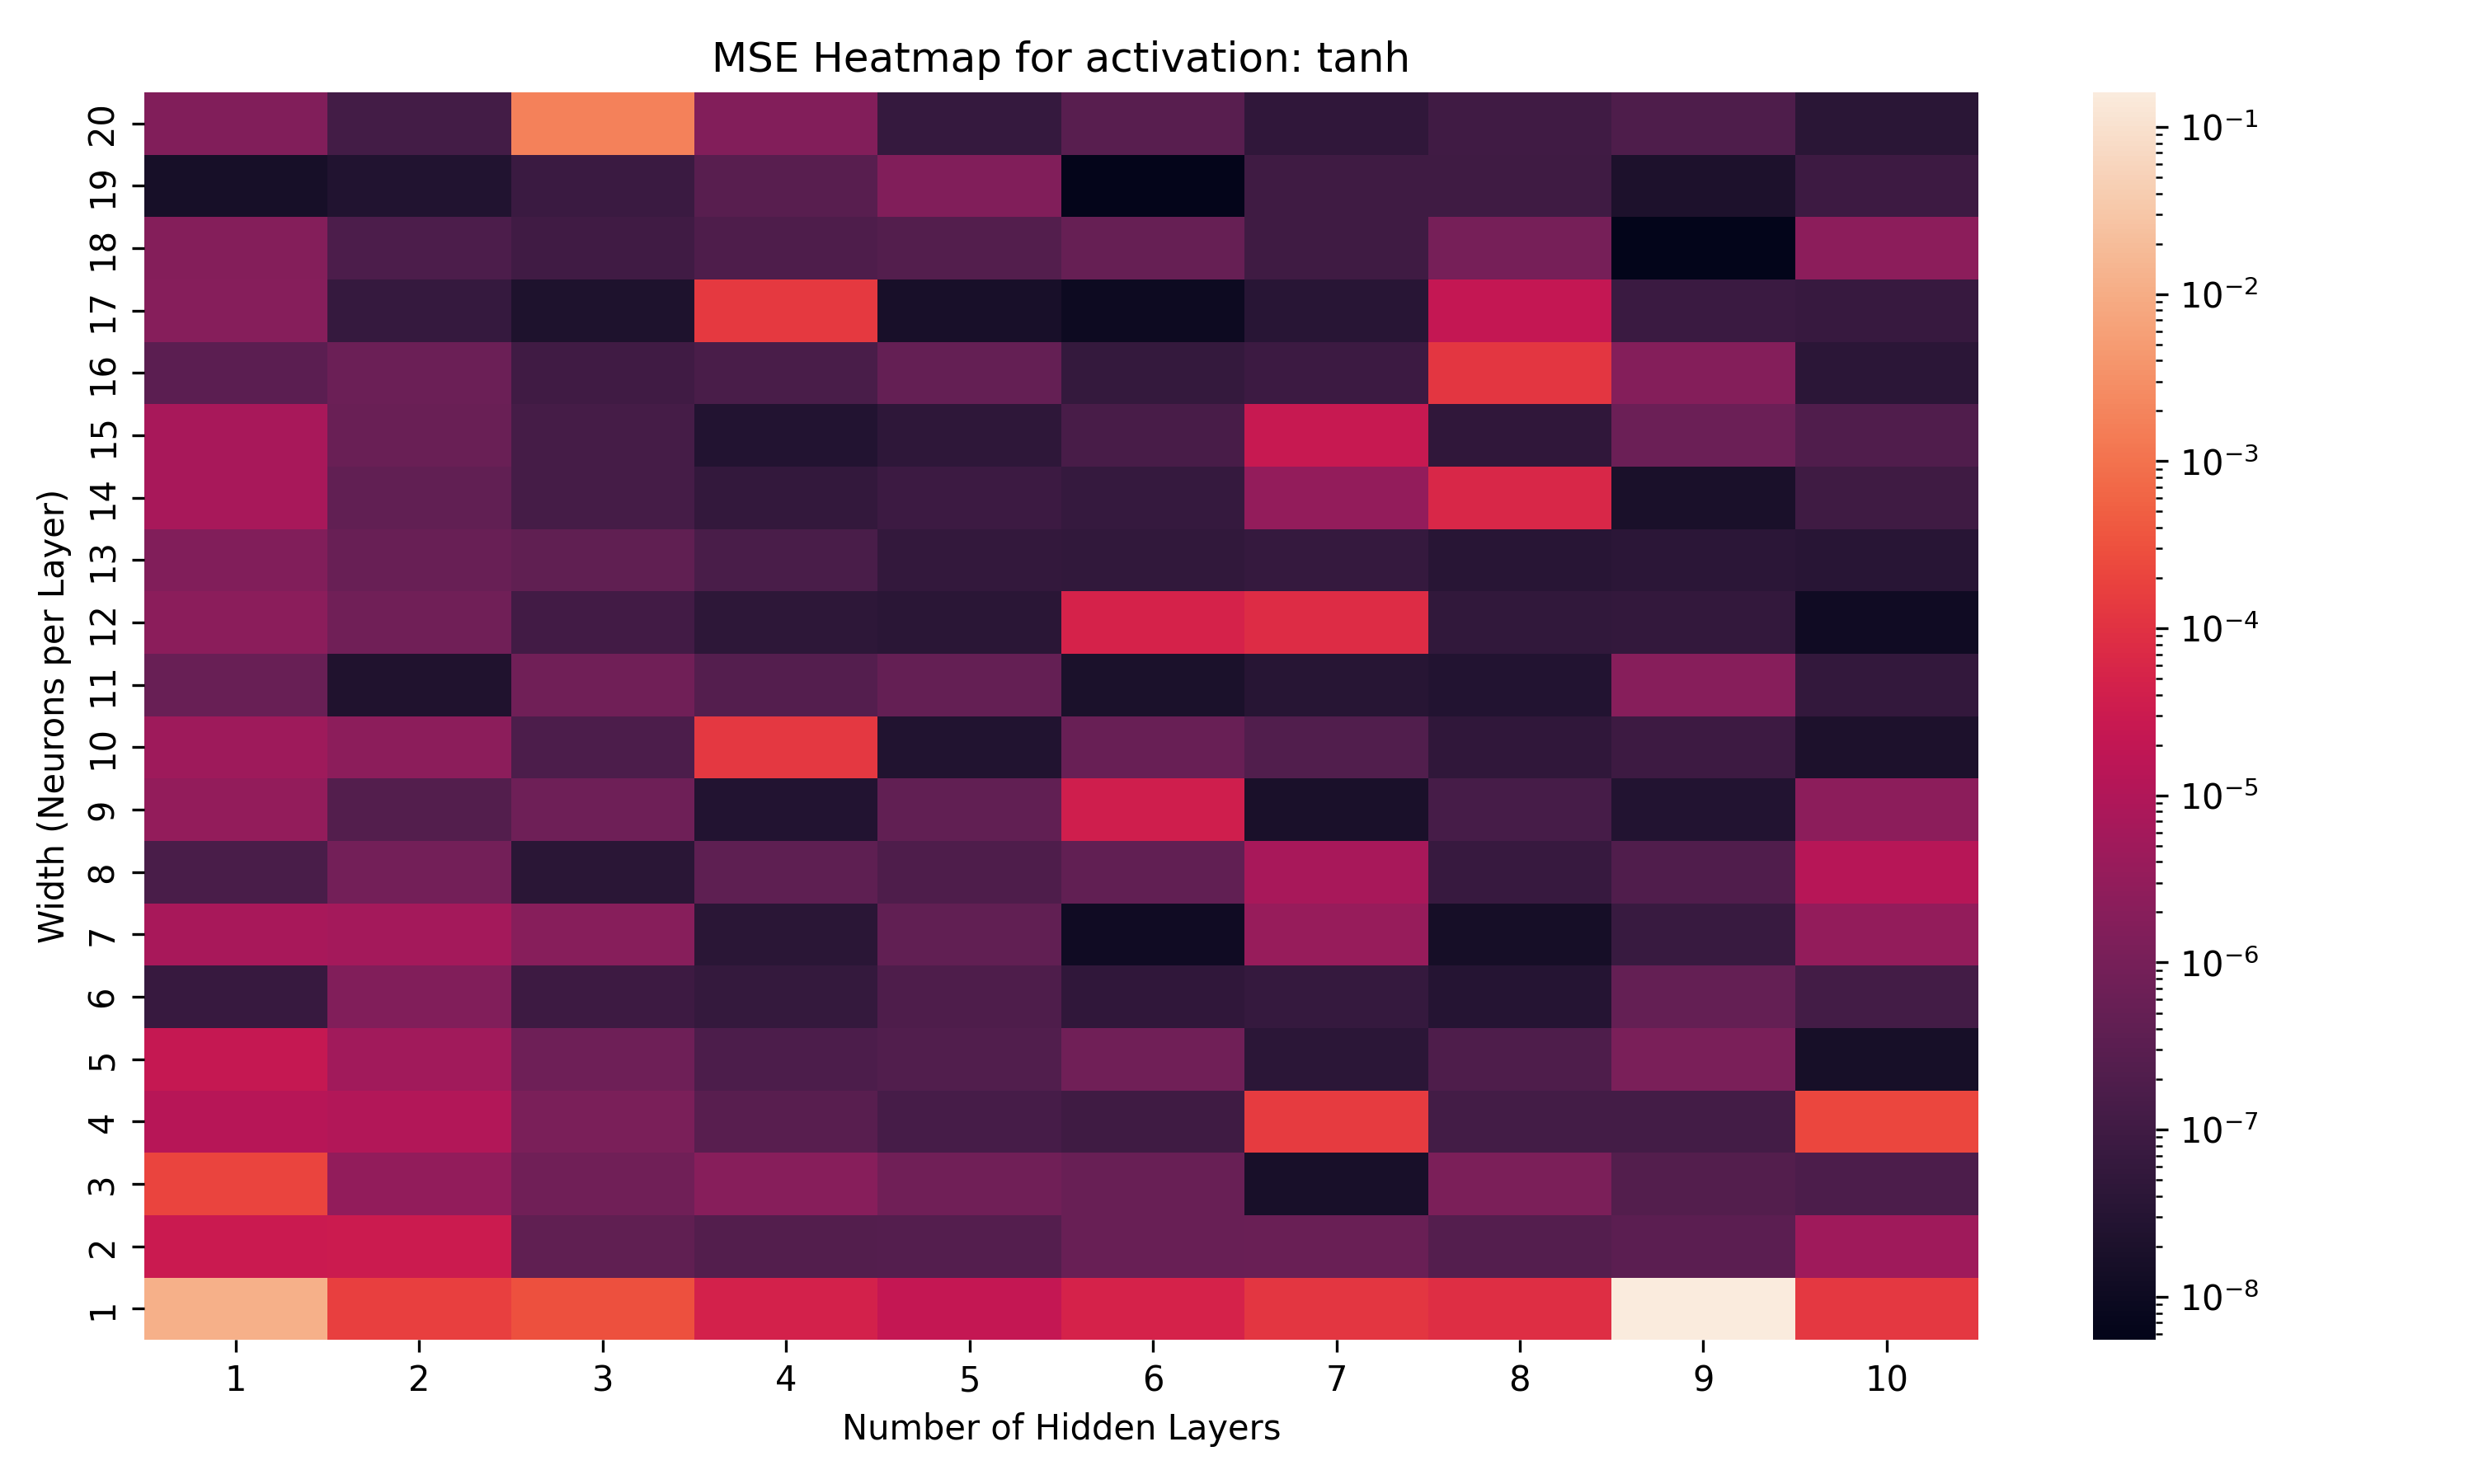
\includegraphics[width=\textwidth]{graphics/mse_heatmap_tanh.png}
        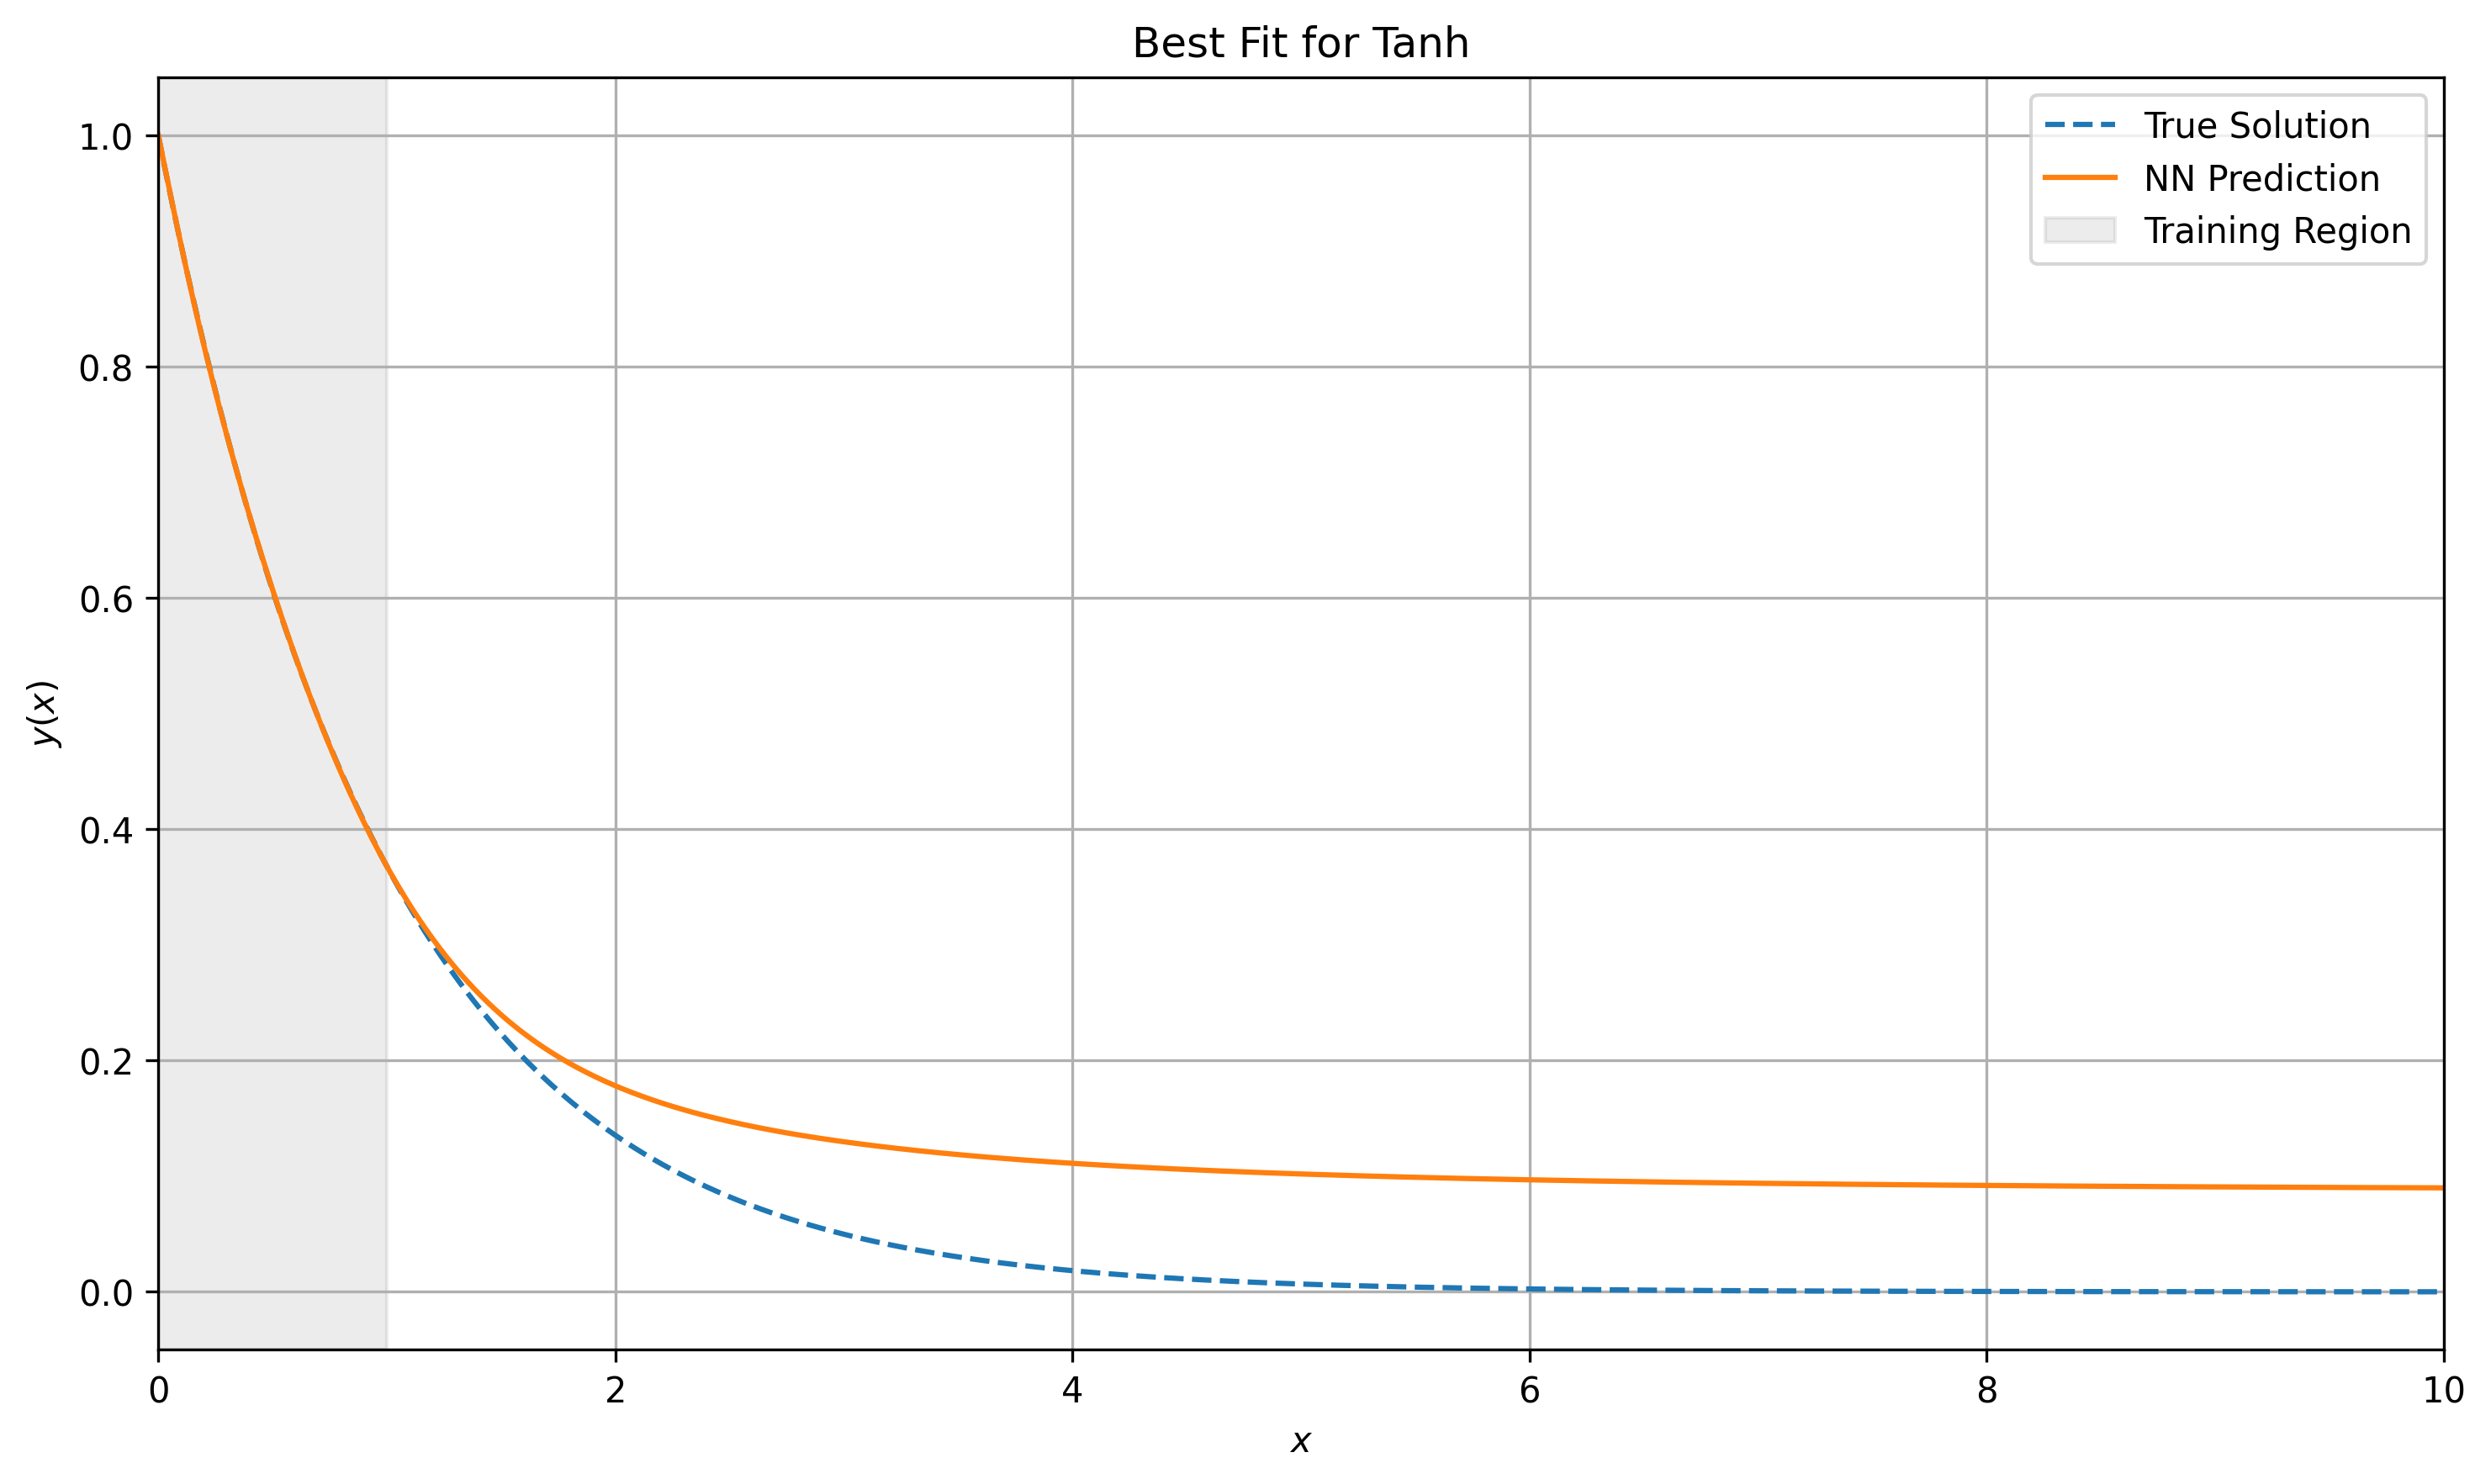
\includegraphics[width=\textwidth]{graphics/best_fit_tanh_6layers_15width.png}
        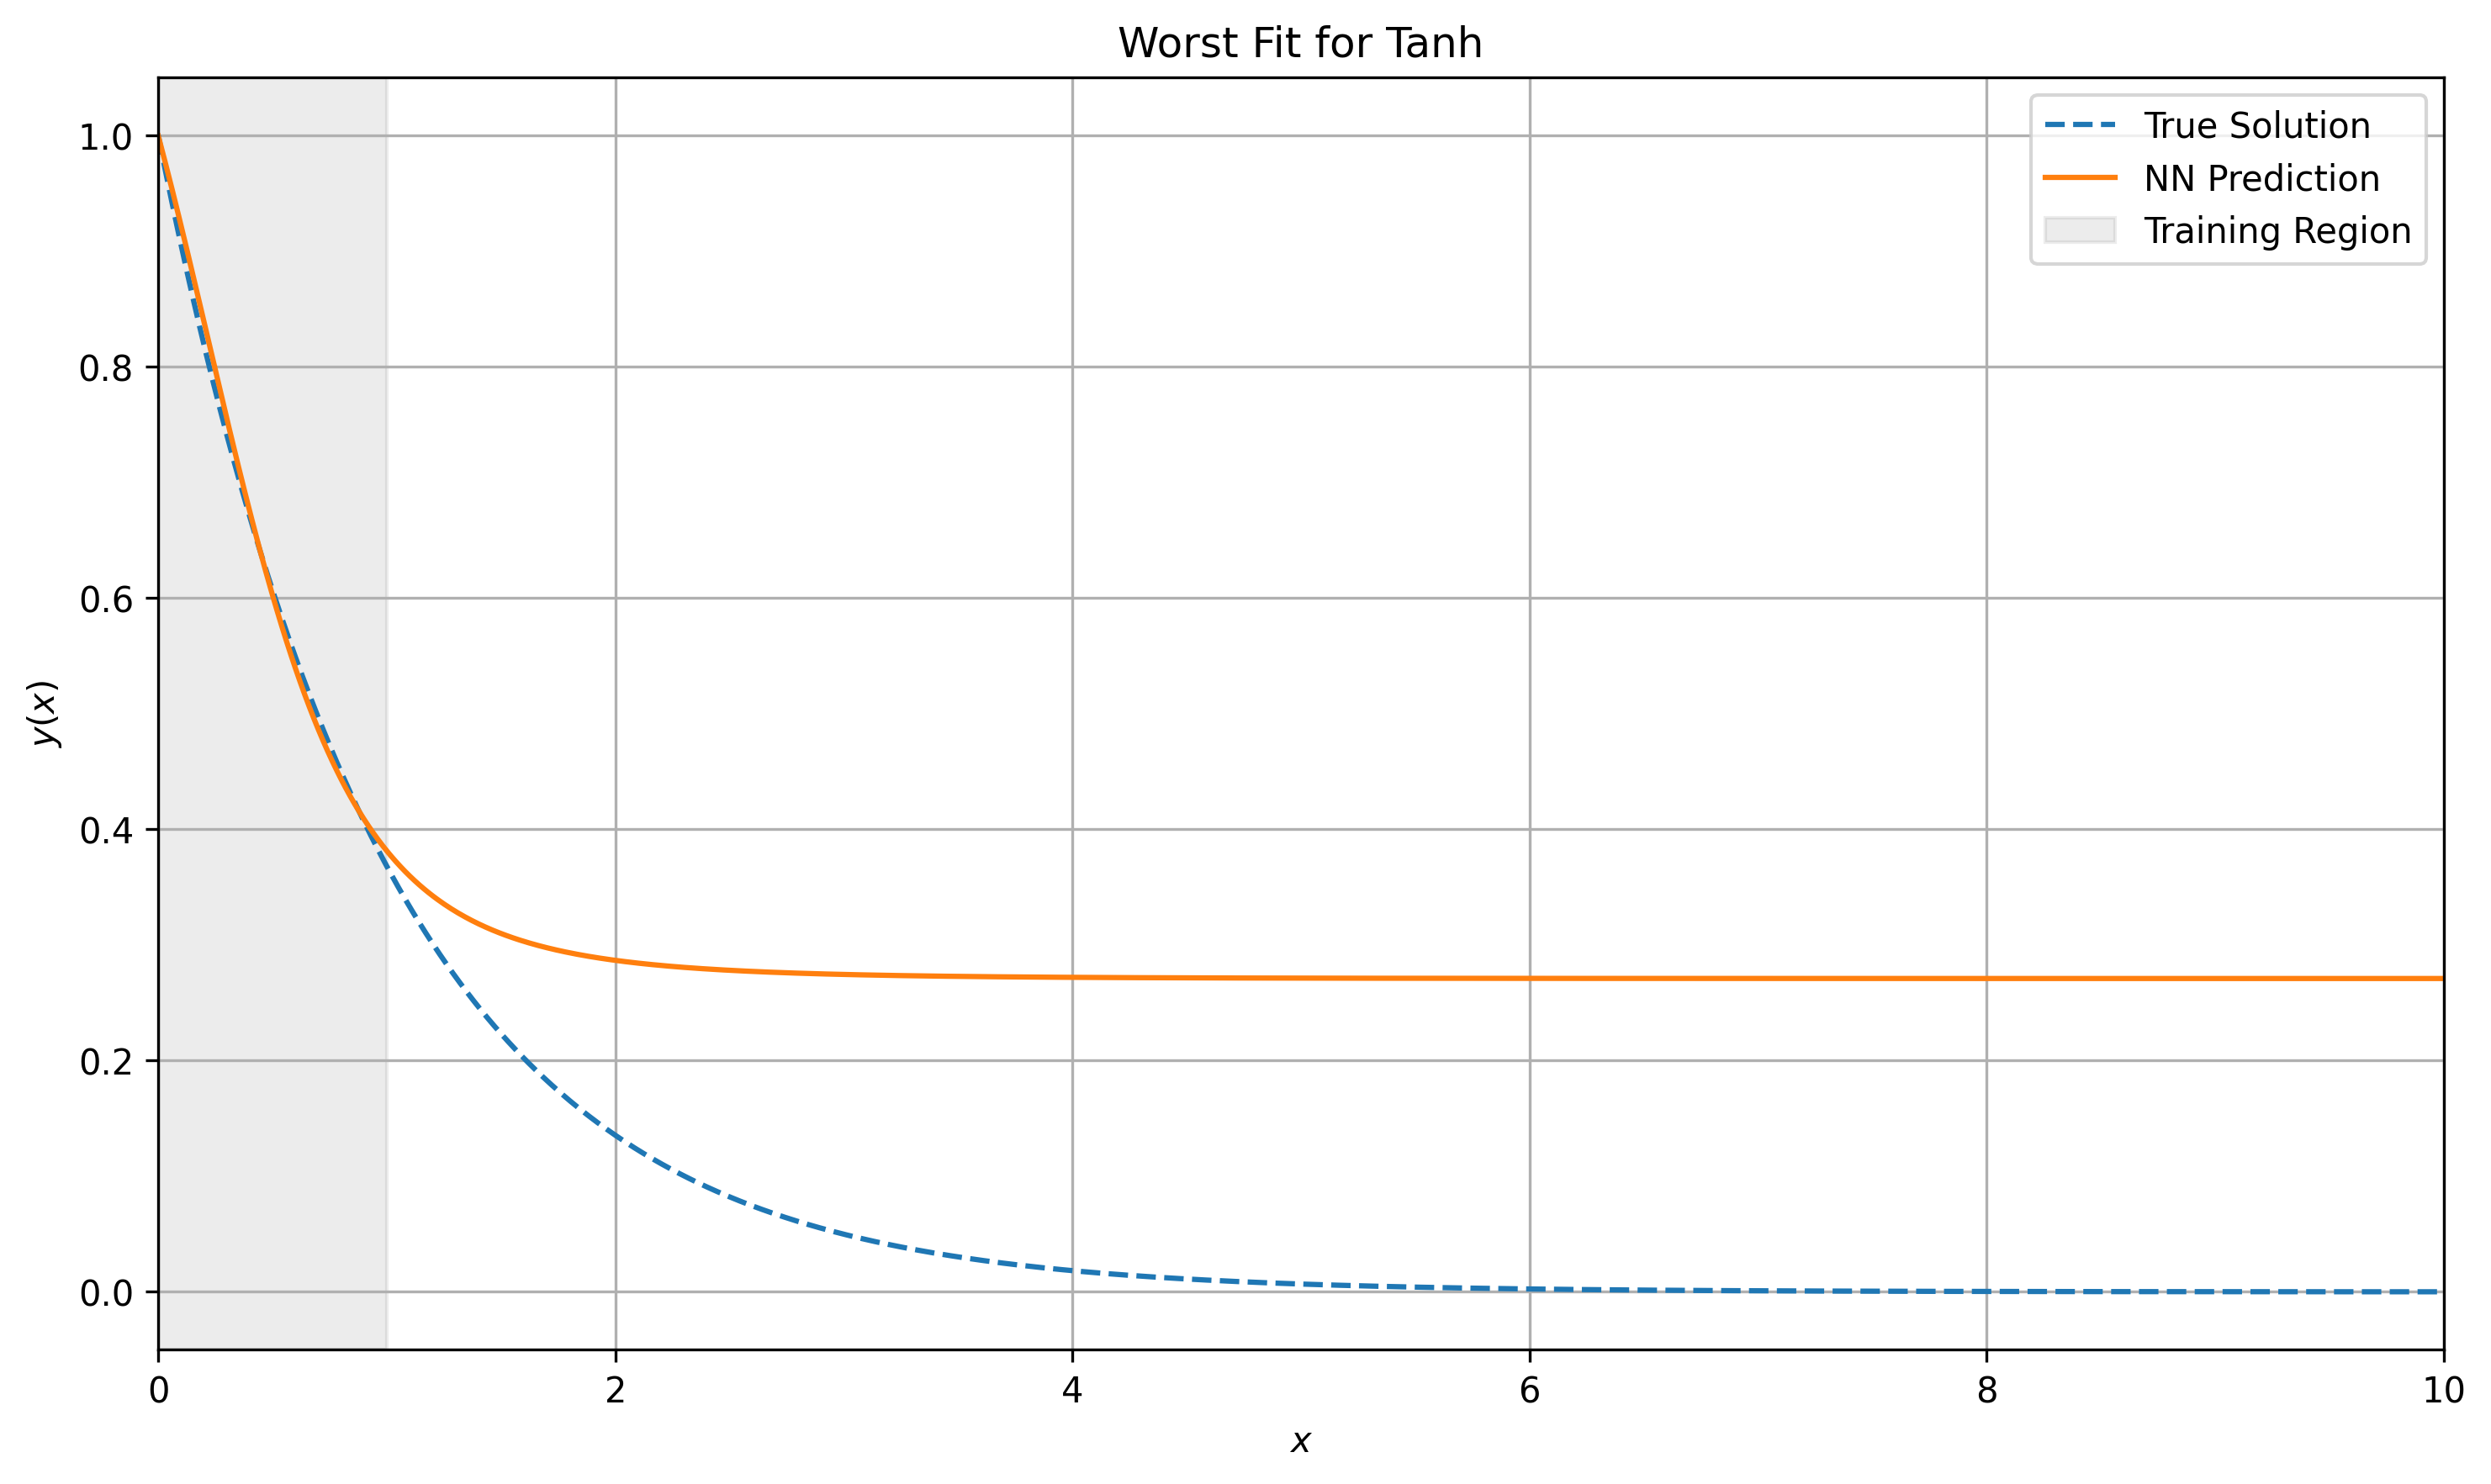
\includegraphics[width=\textwidth]{graphics/worst_fit_tanh_8layers_1width.png}
        \caption{\textbf{Tanh activation.} Heatmap (top), best fit (middle), and worst fit (bottom).}
        \label{fig:expdecay_tanh_column}
    \end{subfigure}
    \hspace*{\fill}
    \begin{subfigure}[t]{0.48\textwidth}
        \centering
        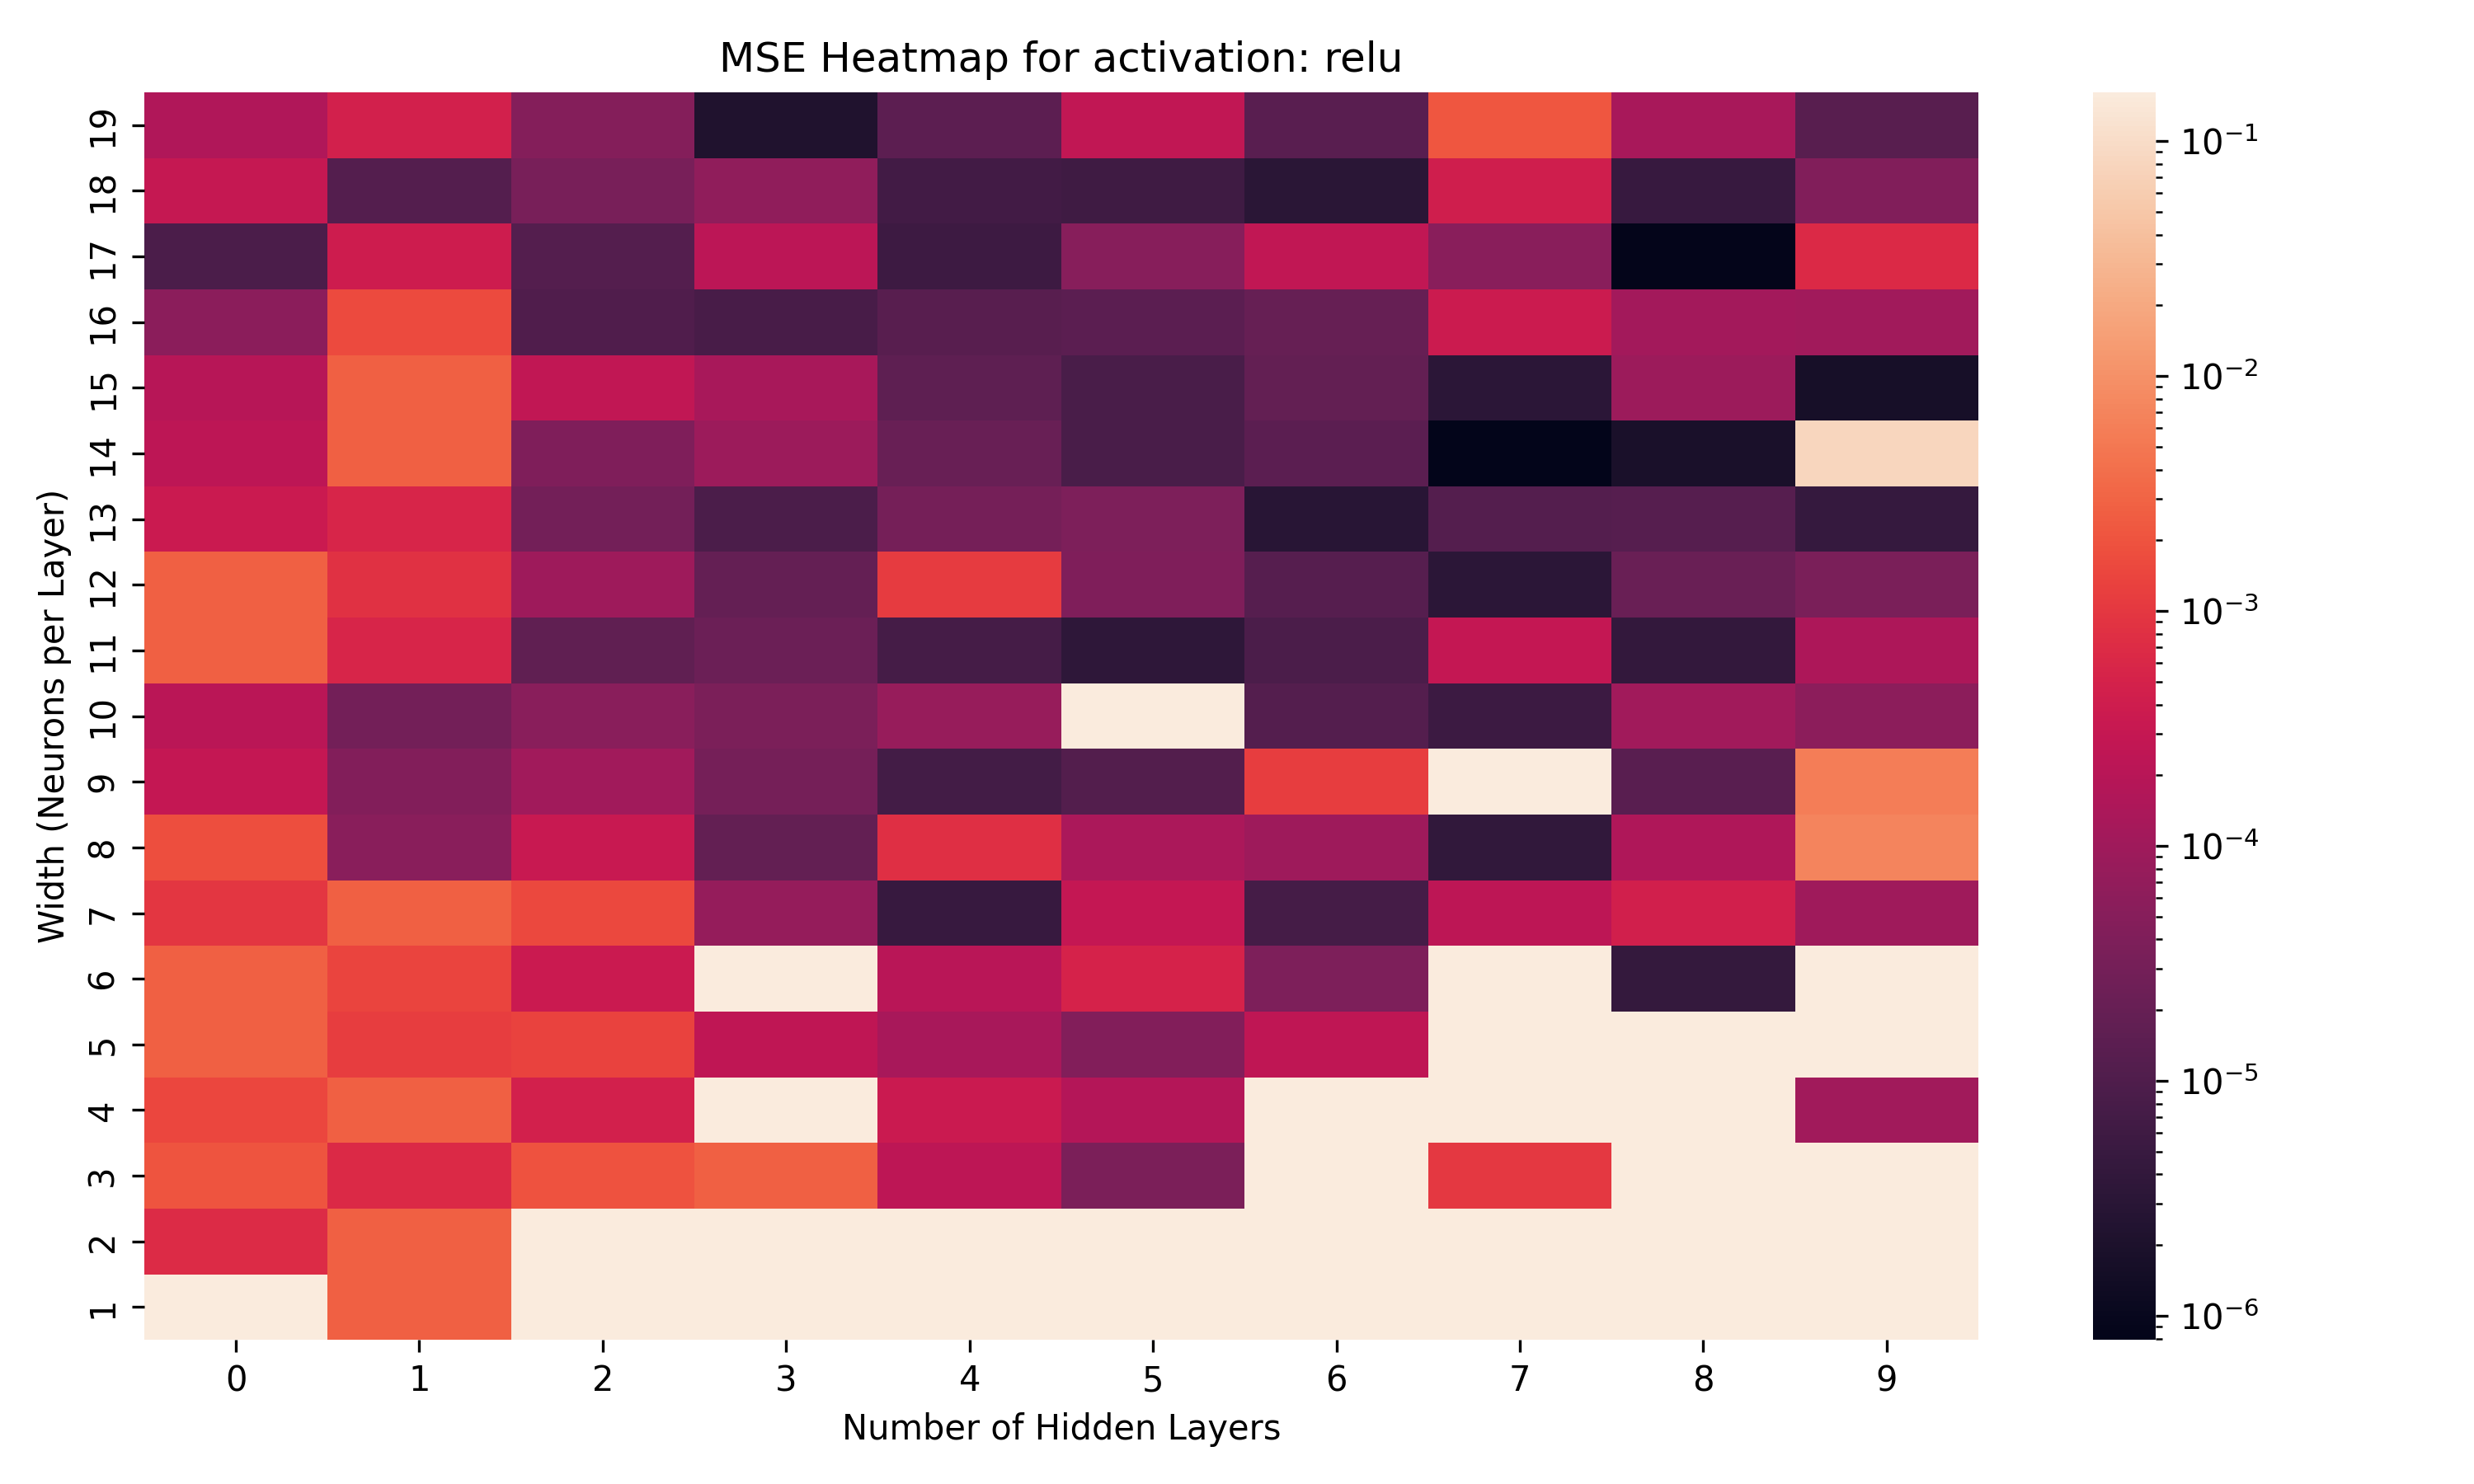
\includegraphics[width=\textwidth]{graphics/mse_heatmap_relu.png}
        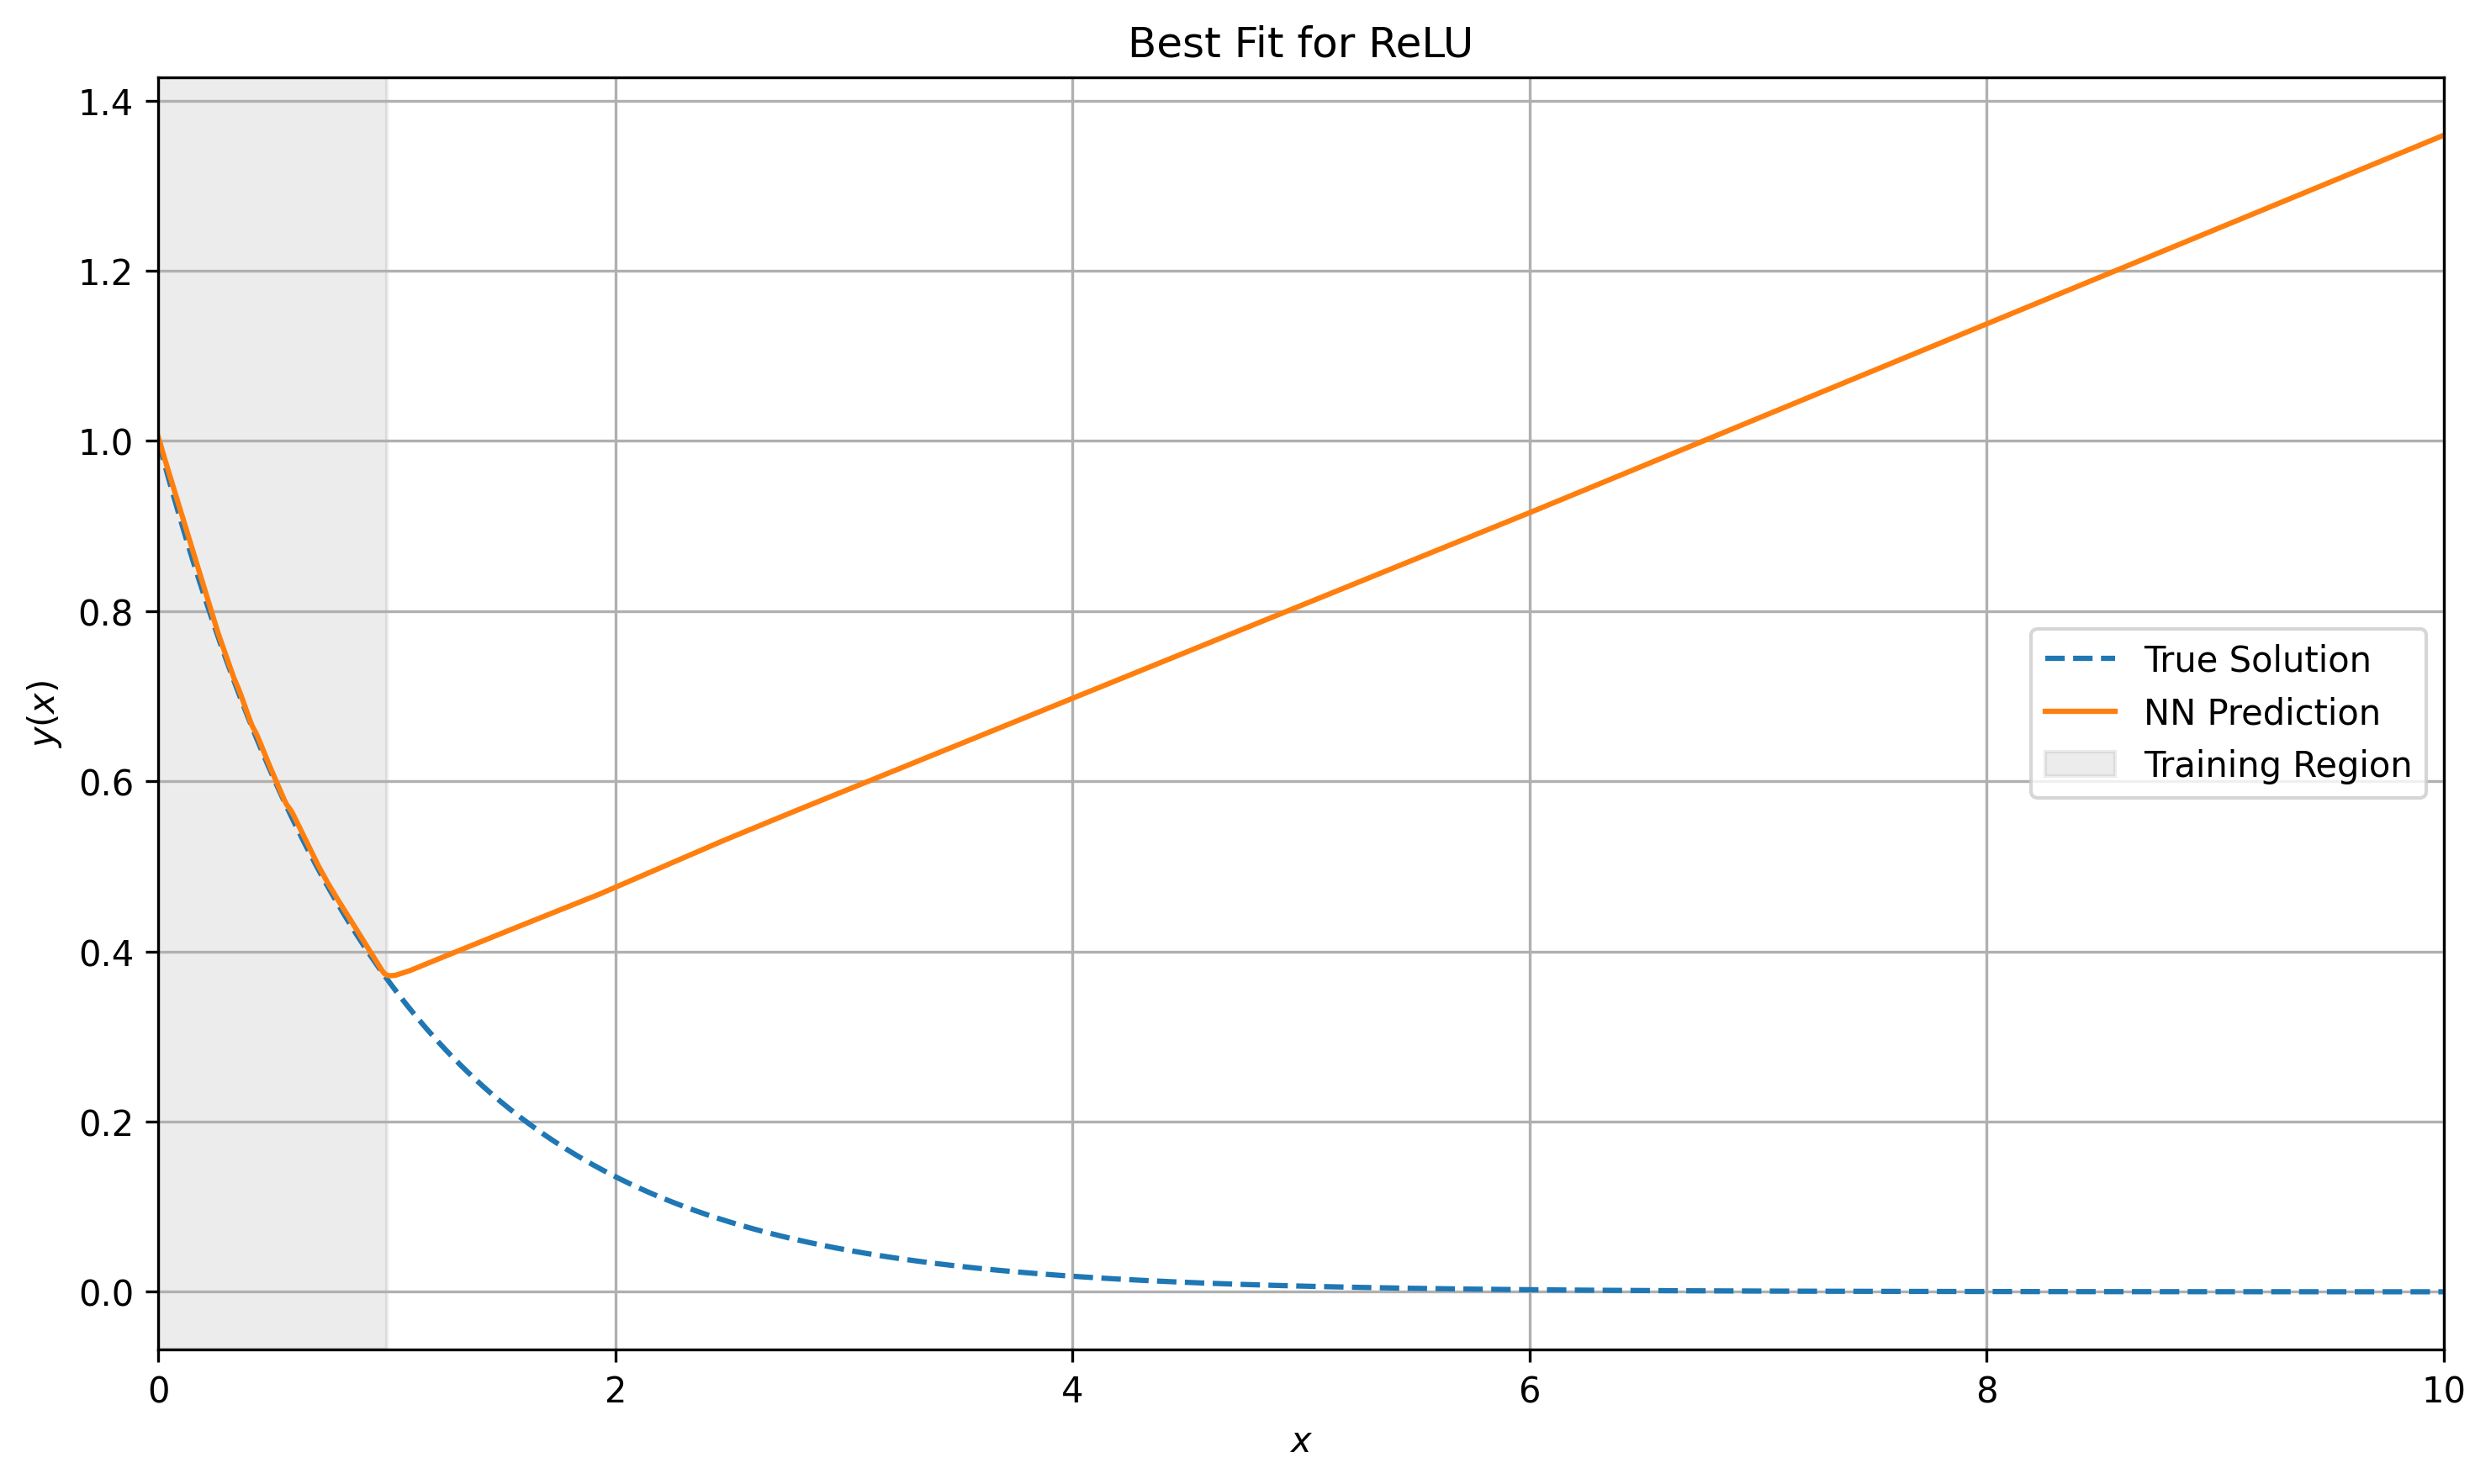
\includegraphics[width=\textwidth]{graphics/best_fit_relu_7layers_14width.png}
        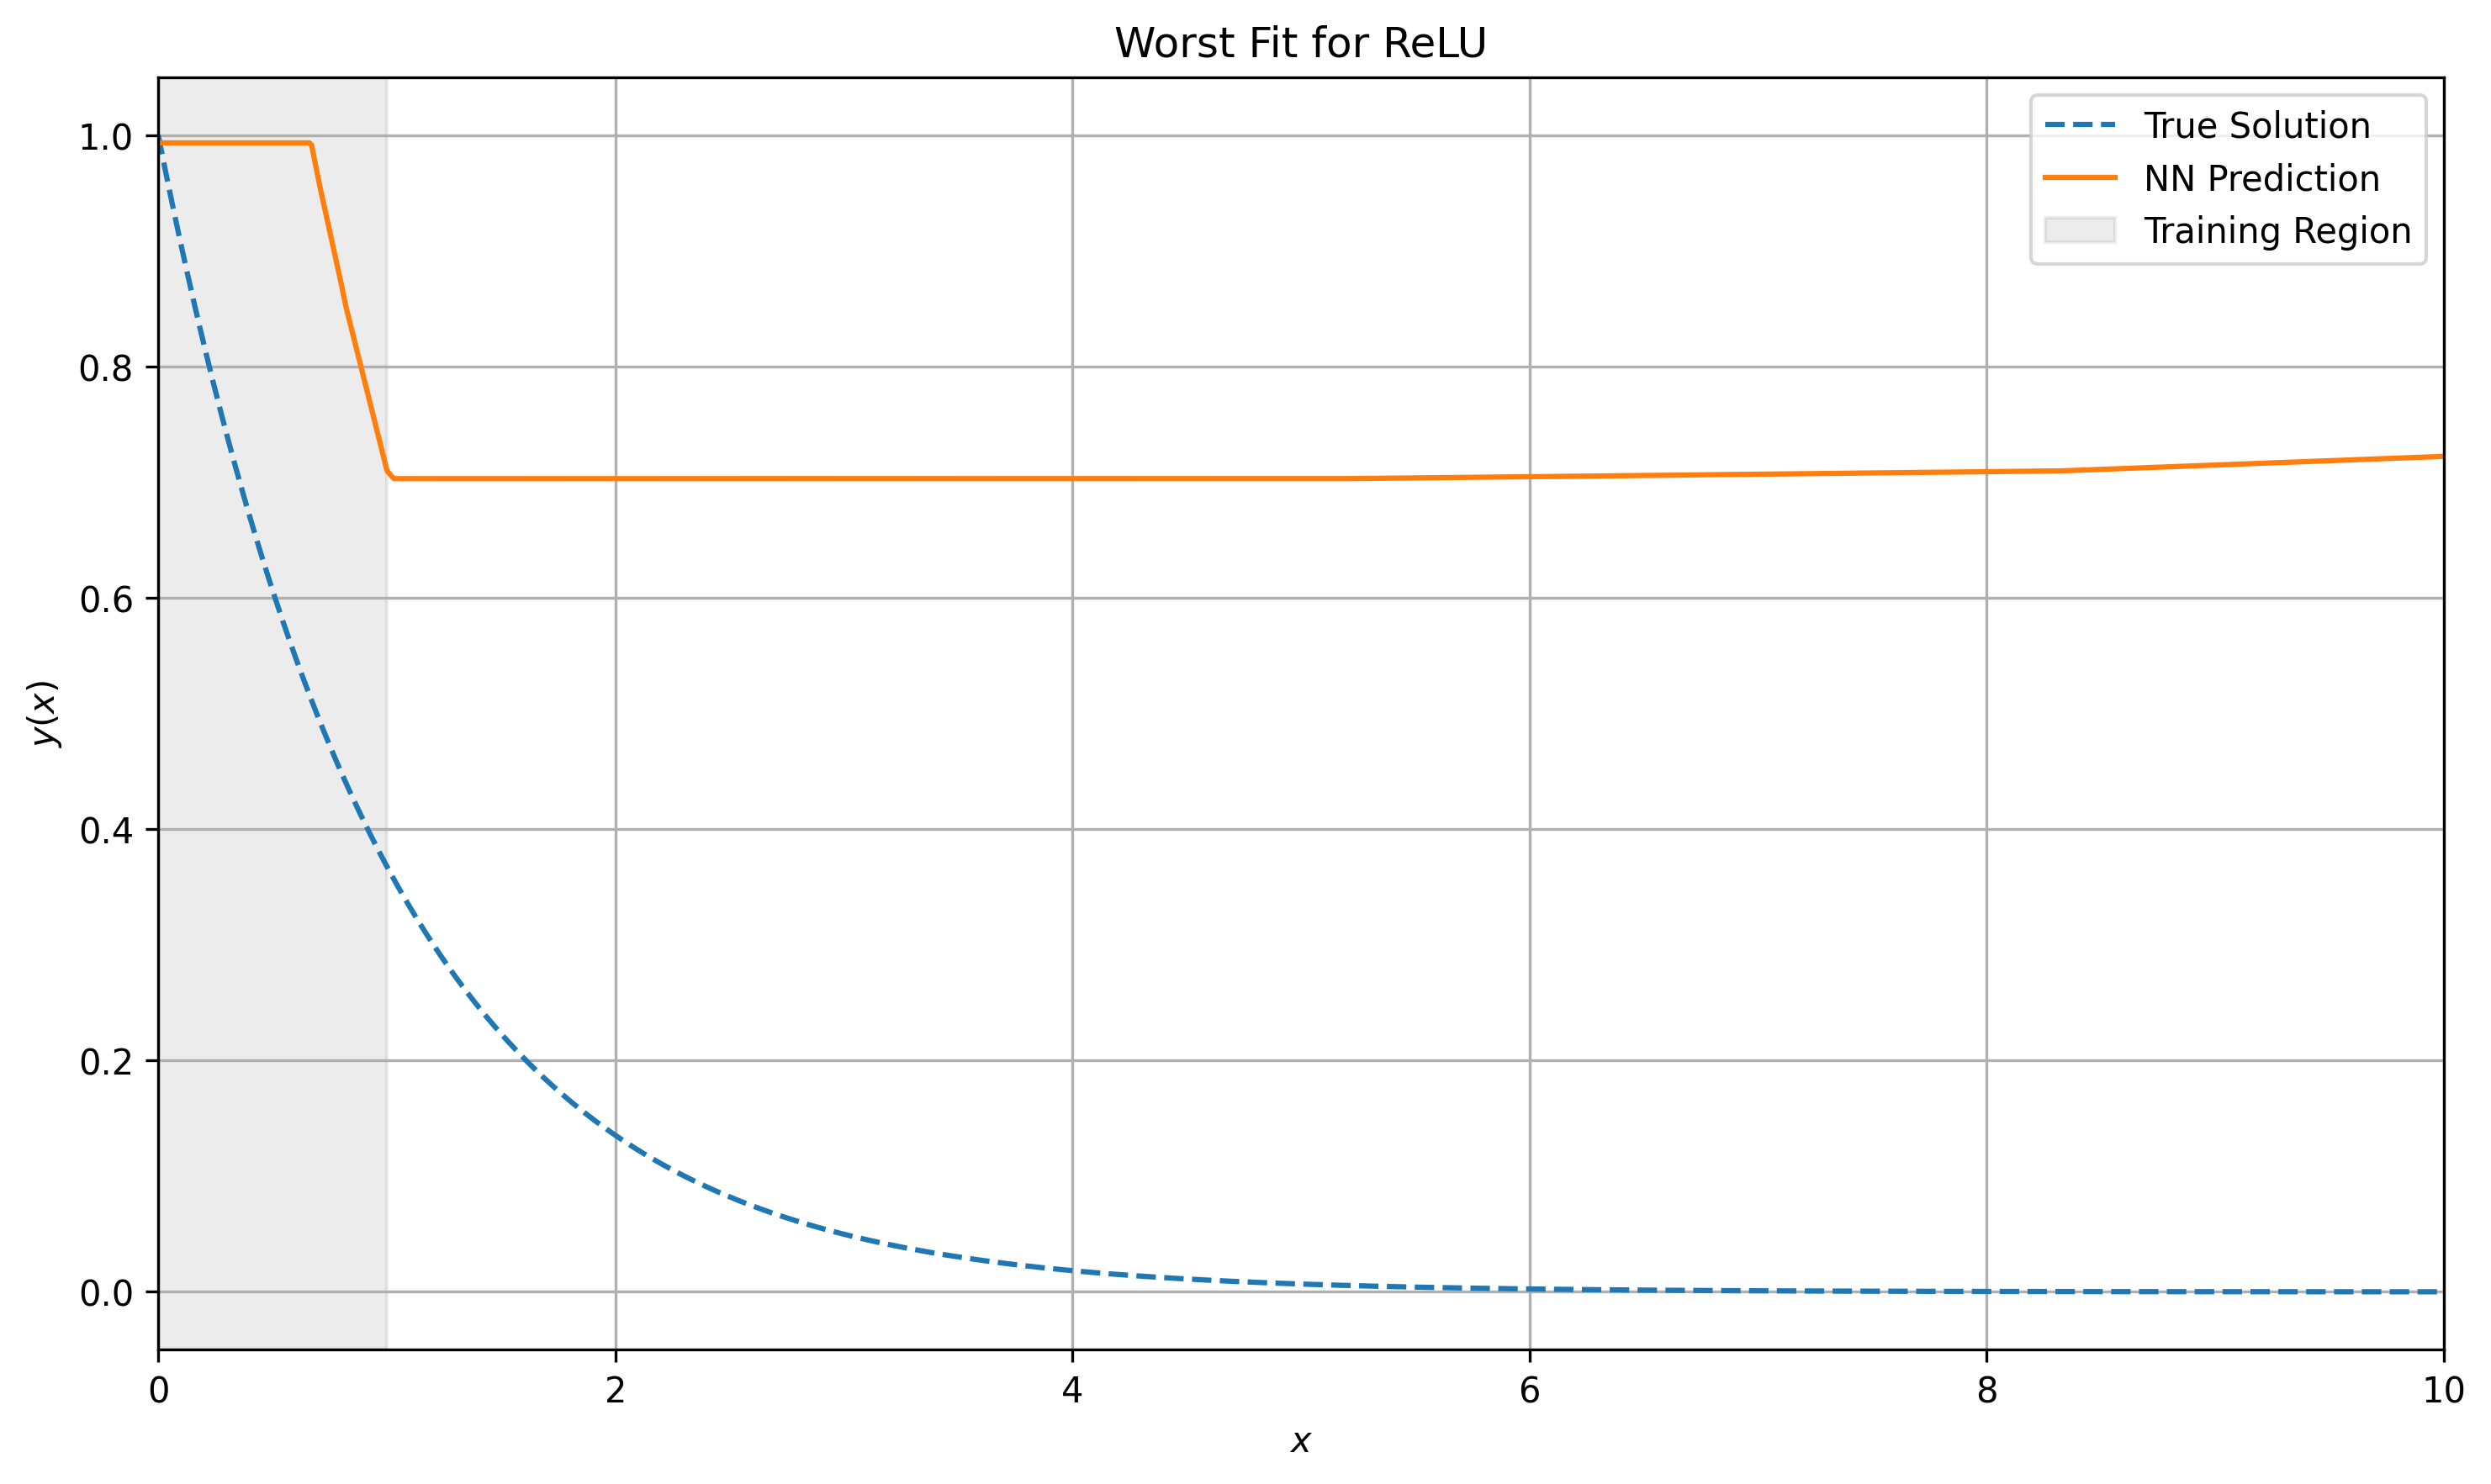
\includegraphics[width=\textwidth]{graphics/worst_fit_relu_7layers_8width.png}
        \caption{\textbf{ReLU activation.} Heatmap (top), best fit (middle), and worst fit (bottom).}
        \label{fig:expdecay_relu_column}
    \end{subfigure}
    \hspace*{\fill}
    \caption{Comparison of architectural performance for the exponential decay problem using two 
    activation functions. Each column shows the MSE heatmap with a log error scale,
    the best network fit, and the worst network fit.}
    \label{fig:expdecay_sidebyside}
\end{figure}


The heatmaps in Figure~\ref{fig:expdecay_sidebyside} reveal several consistent trends. For 
both activation functions, increasing the number of neurons per layer generally leads to improved 
accuracy for a fixed number of layers. In contrast, increasing depth alone does not guarantee better 
performance, particularly when layers are narrow. The best-performing configurations are found with 
moderately deep networks (4--8 layers) and wider layers (10--20 neurons), though the overall 
sensitivity to architecture is relatively mild — likely due to the simplicity of the target 
function. More striking differences emerge in extrapolation. The ReLU-based networks fail to 
capture the exponential decay beyond the training domain, typically reverting to a linear 
trajectory. By contrast, the networks trained with \(\tanh\) not only interpolate more accurately 
but also exhibit qualitatively correct exponential behaviour when extrapolated to \(x = 10\).
Notably, the best \(\tanh\) network also performs well in the extrapolated region, while the 
worst-fitting example remains poor throughout. Finally, we observe in our heatmap that the 
error for most neural network architectures using the $\tanh$ activation function has lower MSE 
than those using the ReLu function. 



\paragraph{Periodic Solution}

We now consider an initial value problem whose solution is periodic:
\[
\begin{aligned}
    y'(x) &= \cos x, \\
    y(0) &= 0.
\end{aligned}
\]
The exact solution is \( y(x) = \sin x \), which is smooth, bounded, and periodic with period \( 2\pi \).  
This problem allows us to evaluate the capacity of neural networks to approximate oscillatory behaviour
across a wide domain, and to test whether the learned solution generalises beyond a single period.

We perform the same analysis as in the previous section, first analysing how the error varies
for different architectures, and then examining best solutions (we exclude the worst 
cases now, as these were purely for comparison to best in the preceding section), shown in Figure 
\ref{fig:ivp_periodic_sidebyside}.

\begin{figure}[h]
    \centering
    \hspace*{\fill}
    \begin{subfigure}[t]{0.48\textwidth}
        \centering
        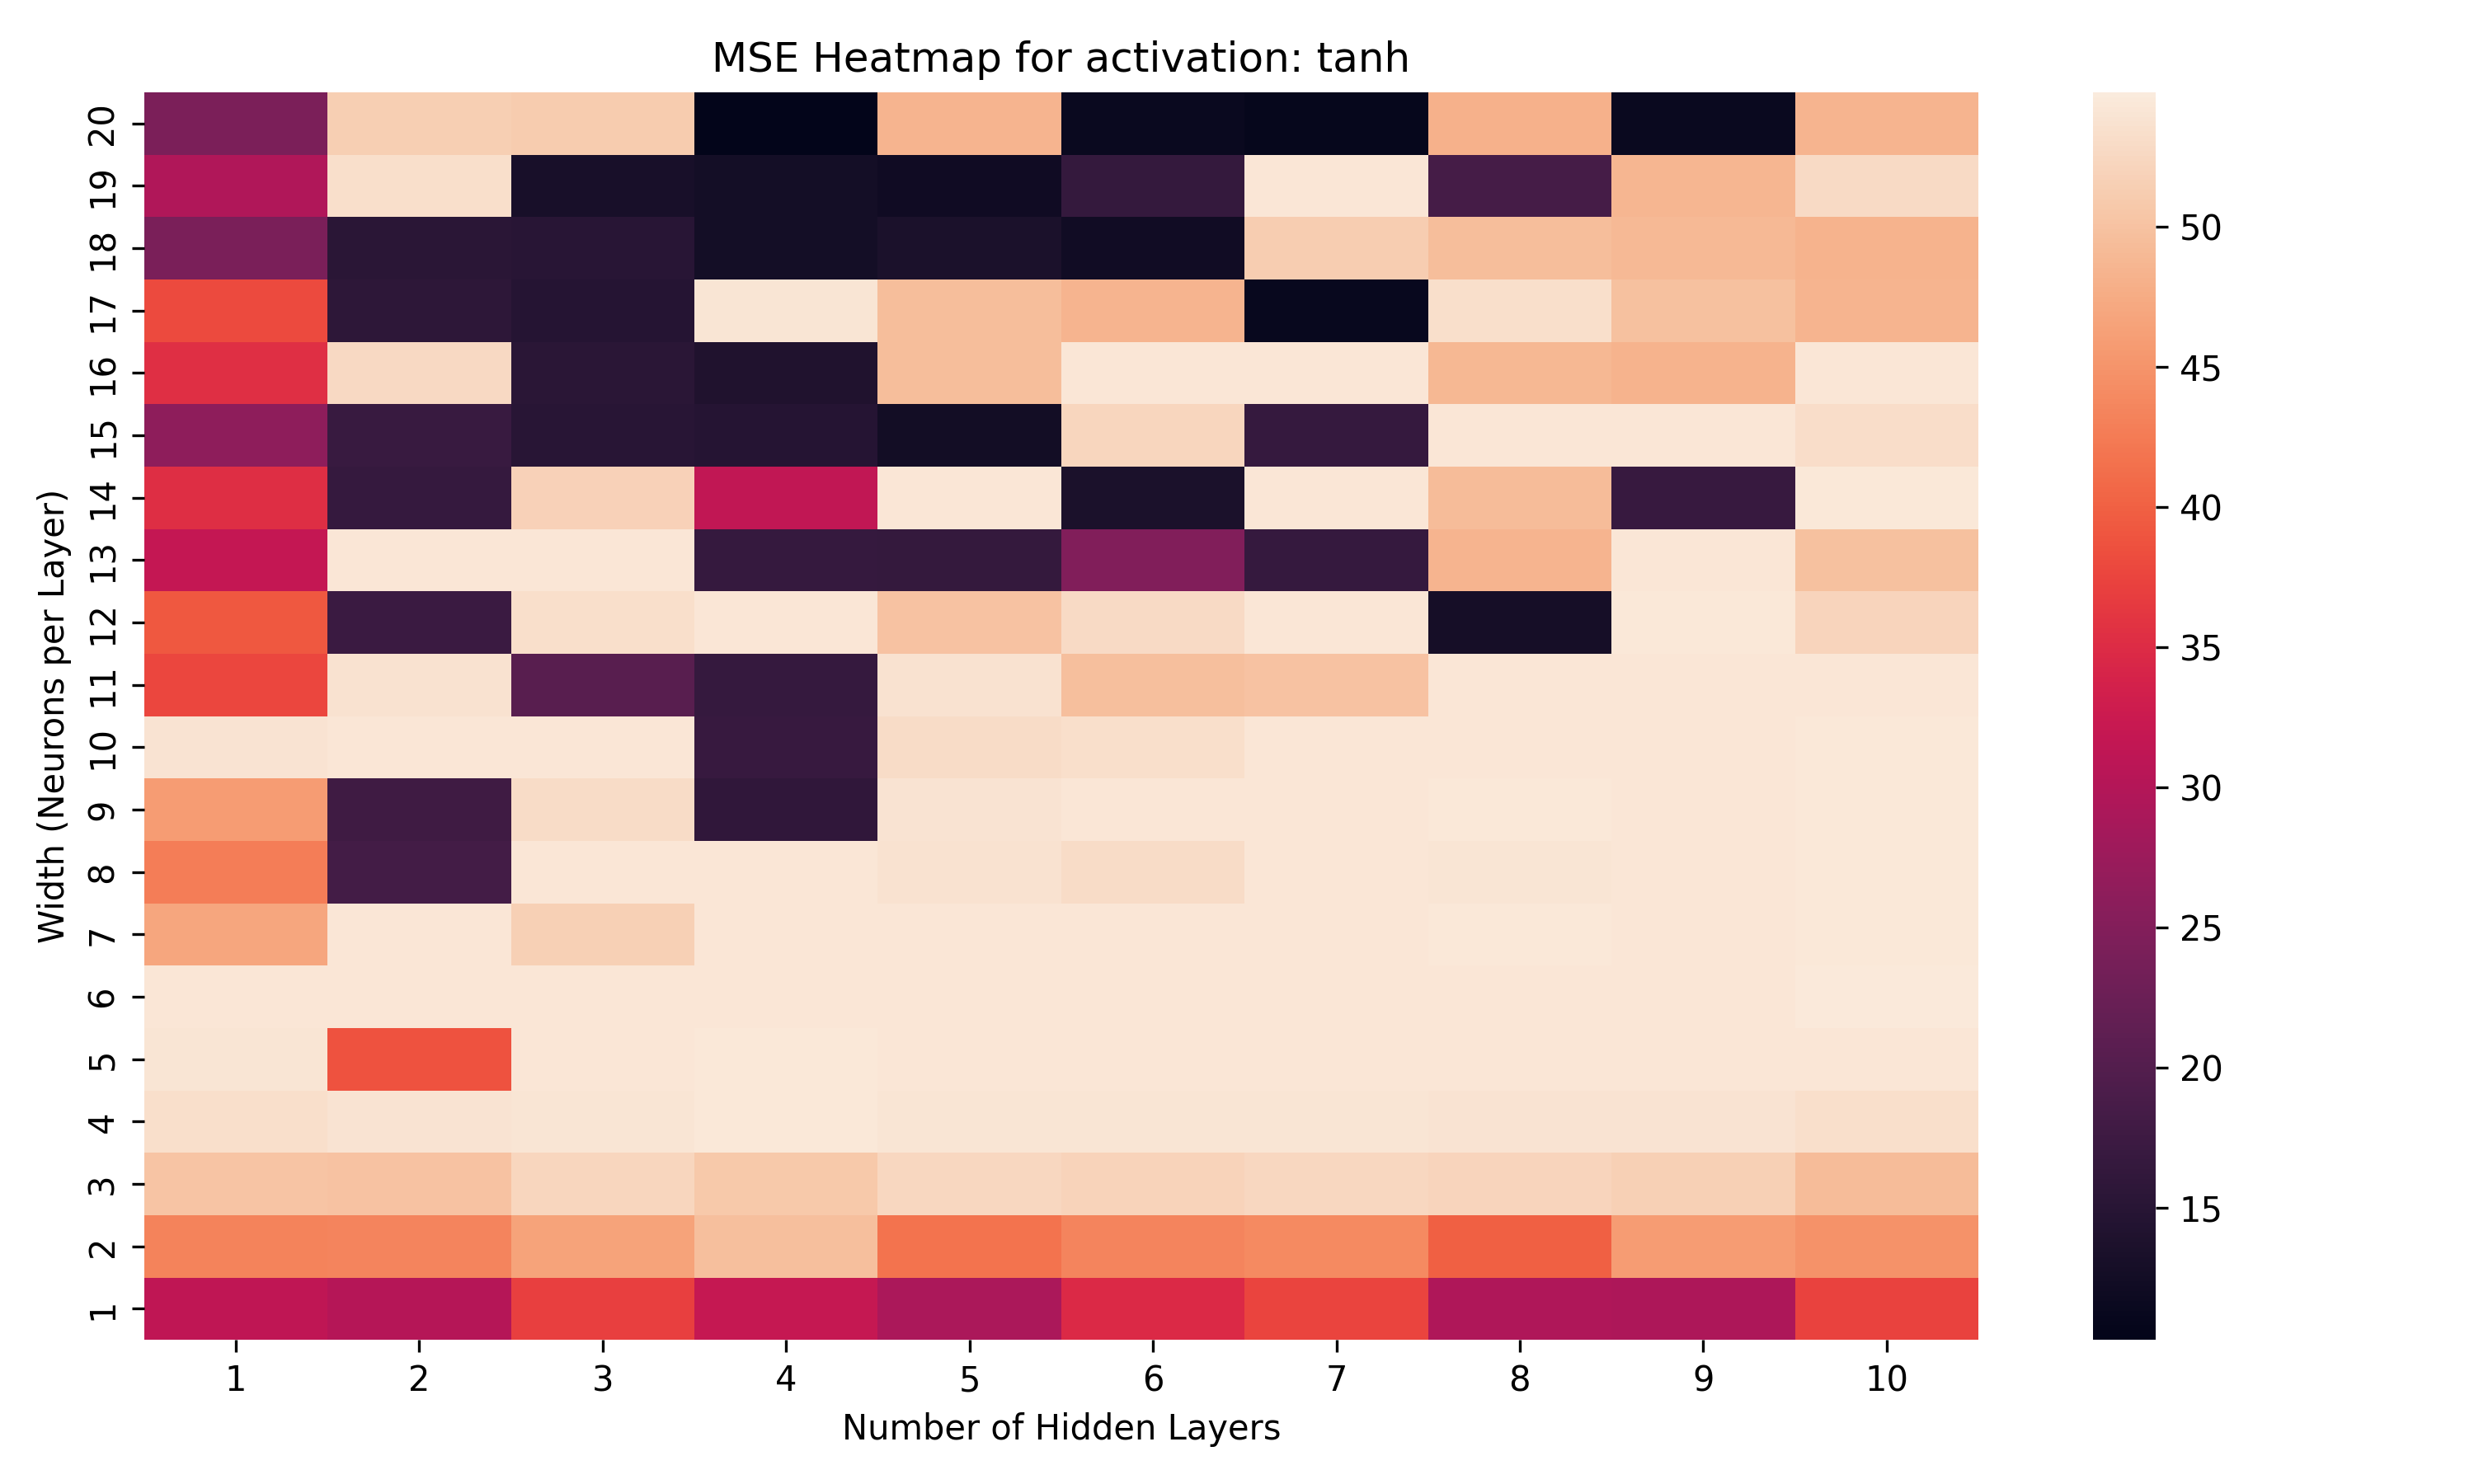
\includegraphics[width=\textwidth]{graphics/mse_heatmap_ivp_periodic_tanh.png}
        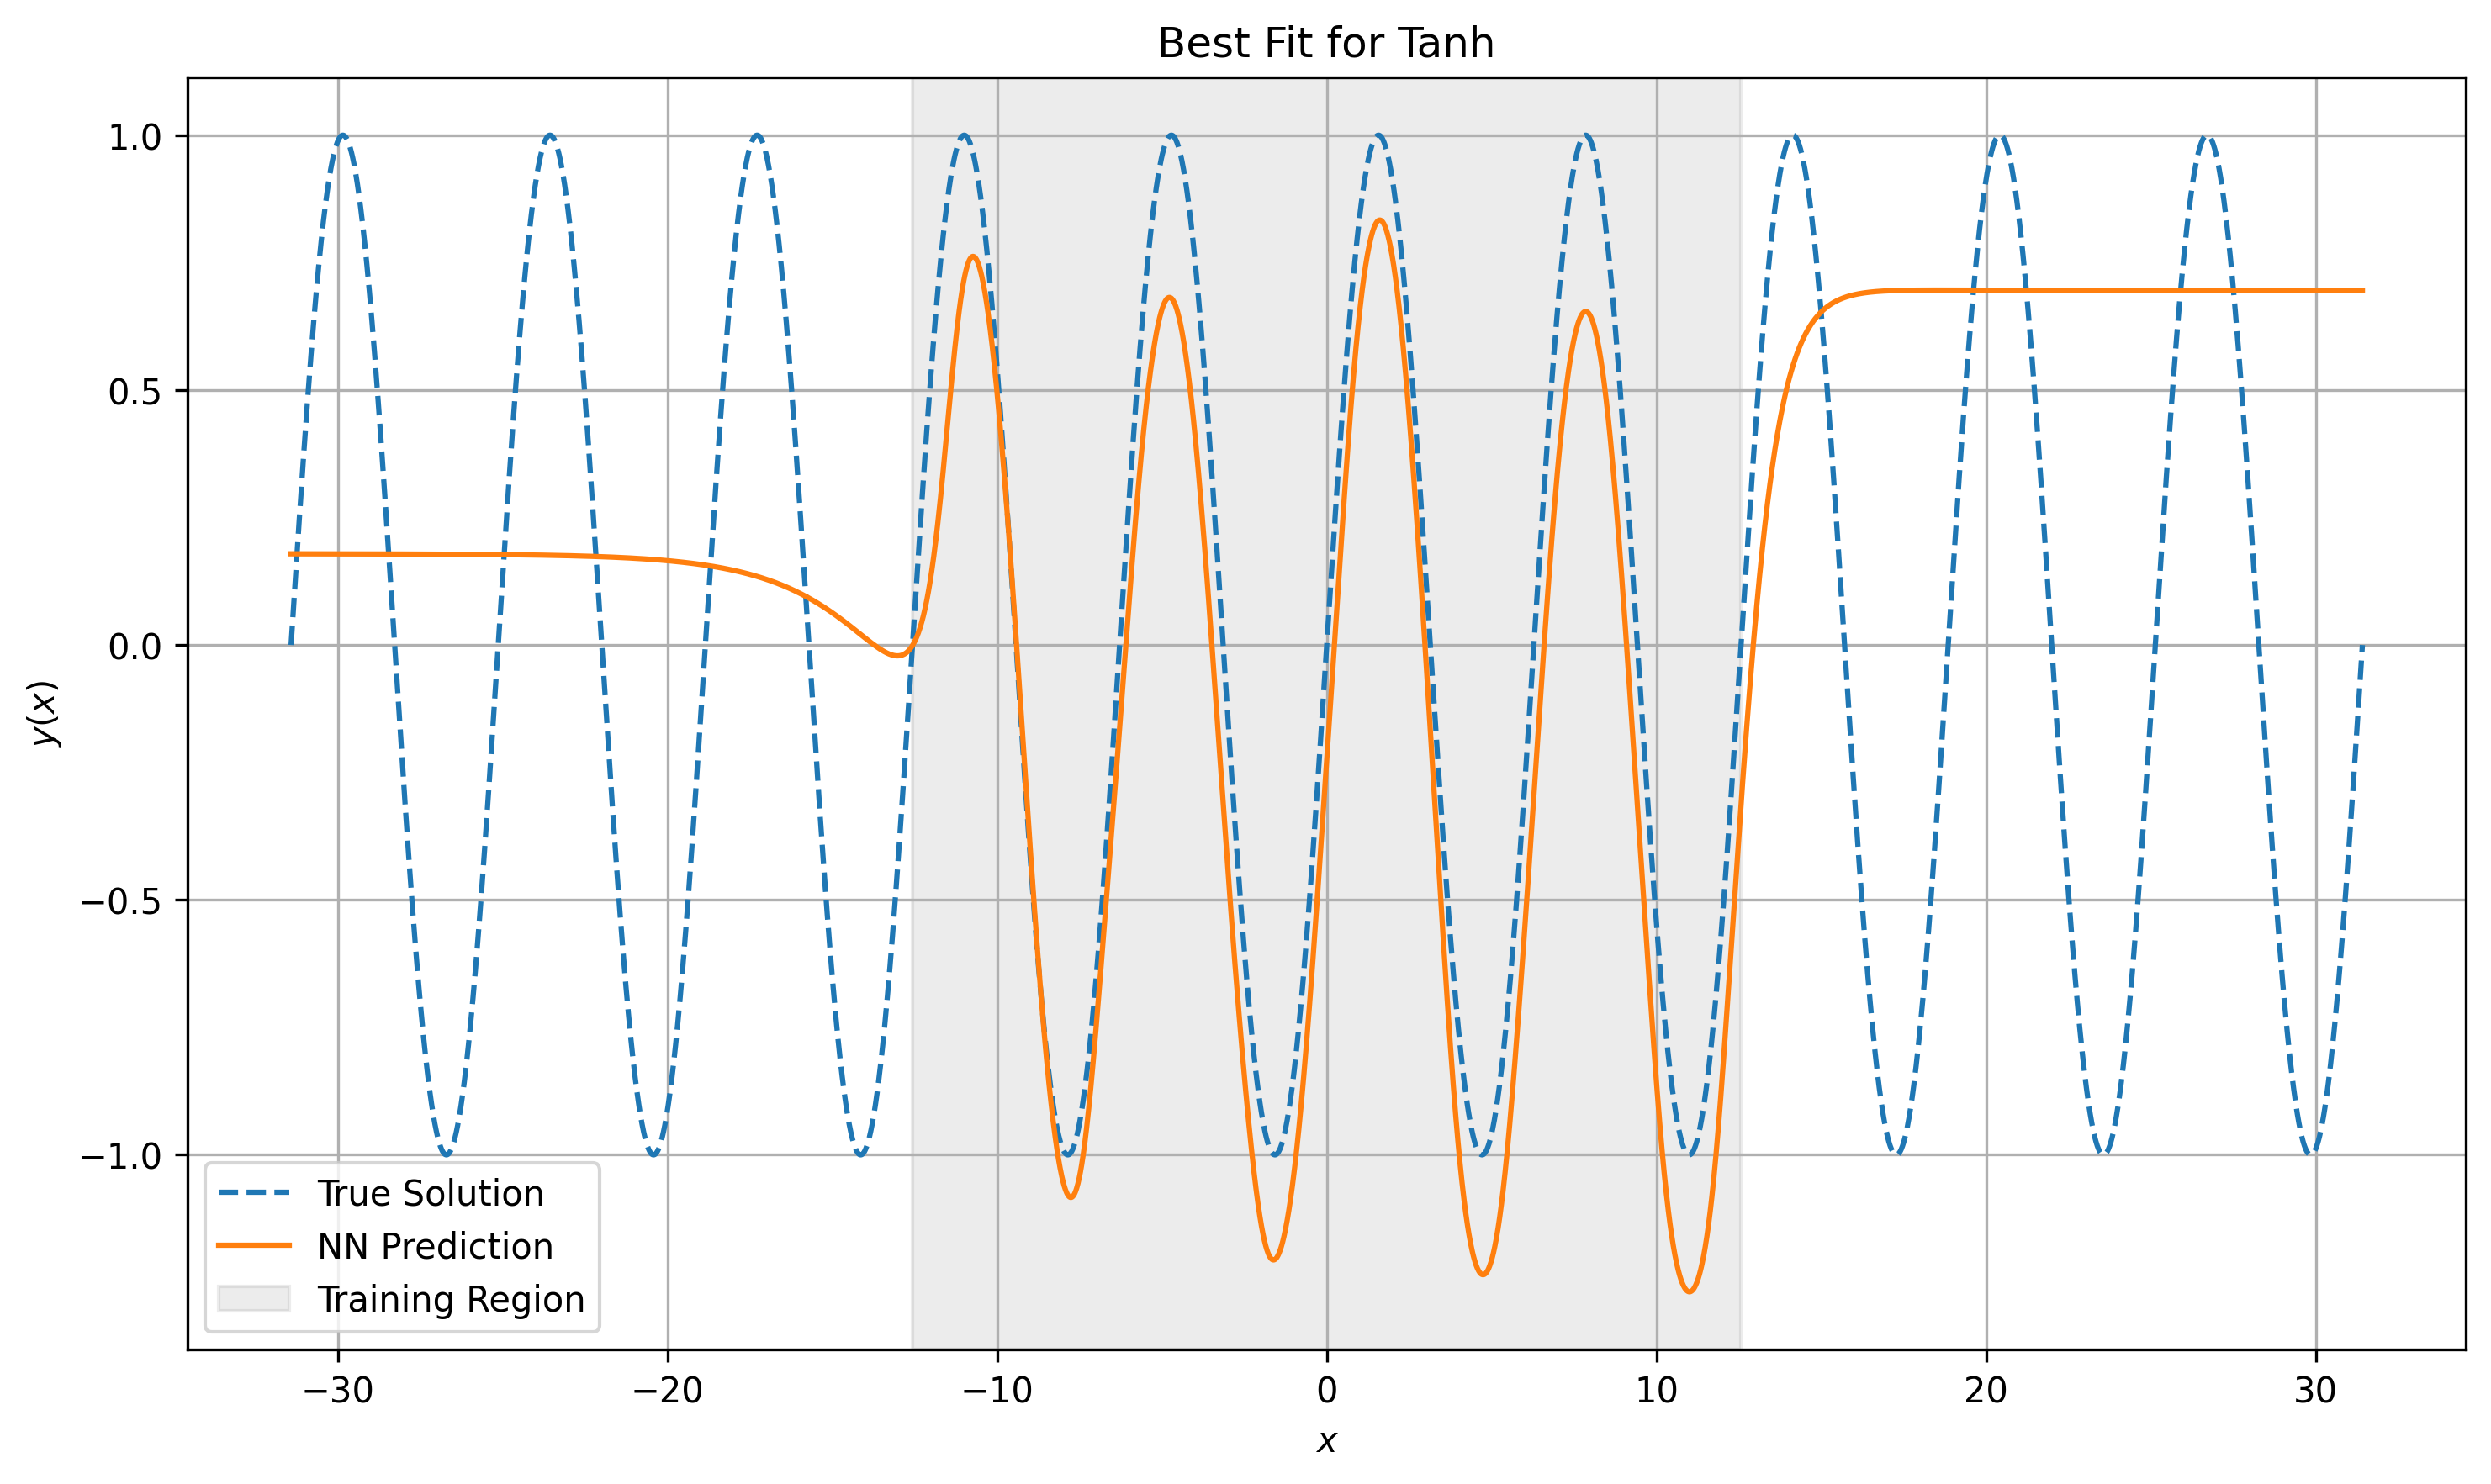
\includegraphics[width=\textwidth]{graphics/ivp_periodic_best_fit_tanh_7layers_15width.png}
        \caption{\textbf{Tanh activation.} Heatmap (top), best fit (middle), and worst fit (bottom).}
        \label{fig:ivp_periodic_tanh}
    \end{subfigure}
    \hspace*{\fill}
    \begin{subfigure}[t]{0.48\textwidth}
        \centering
        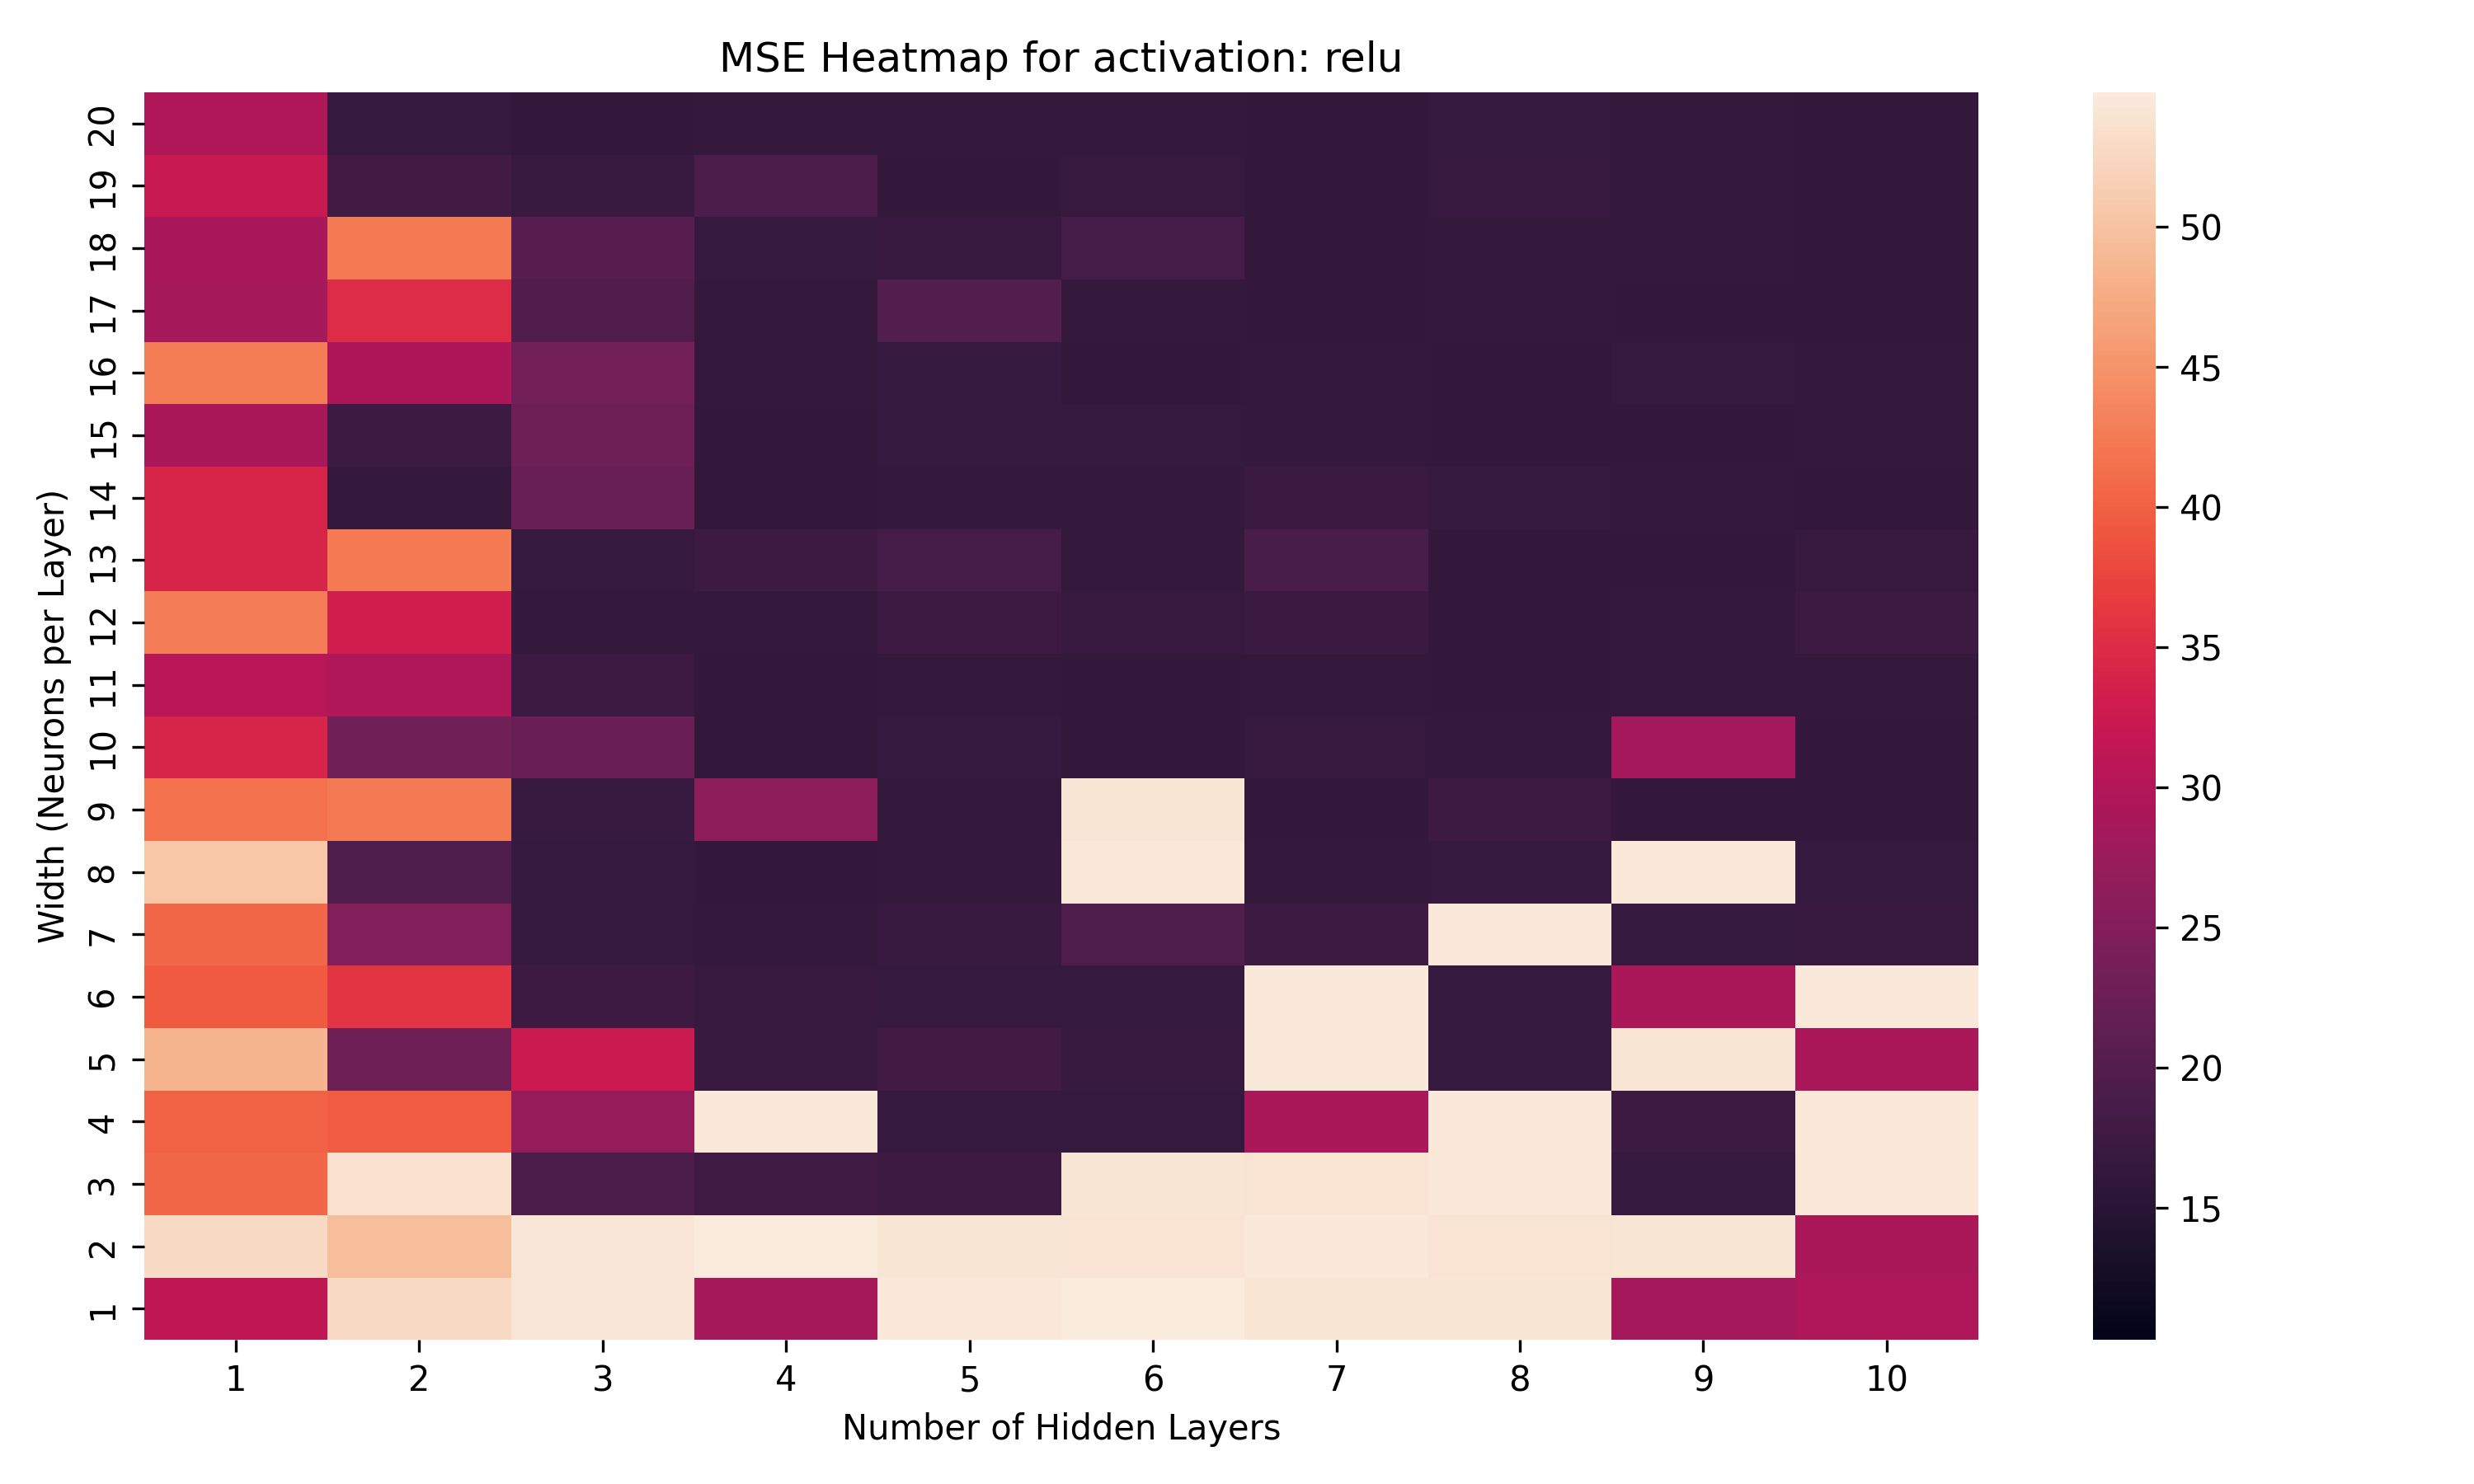
\includegraphics[width=\textwidth]{graphics/mse_heatmap_ivp_periodic_relu.png}
        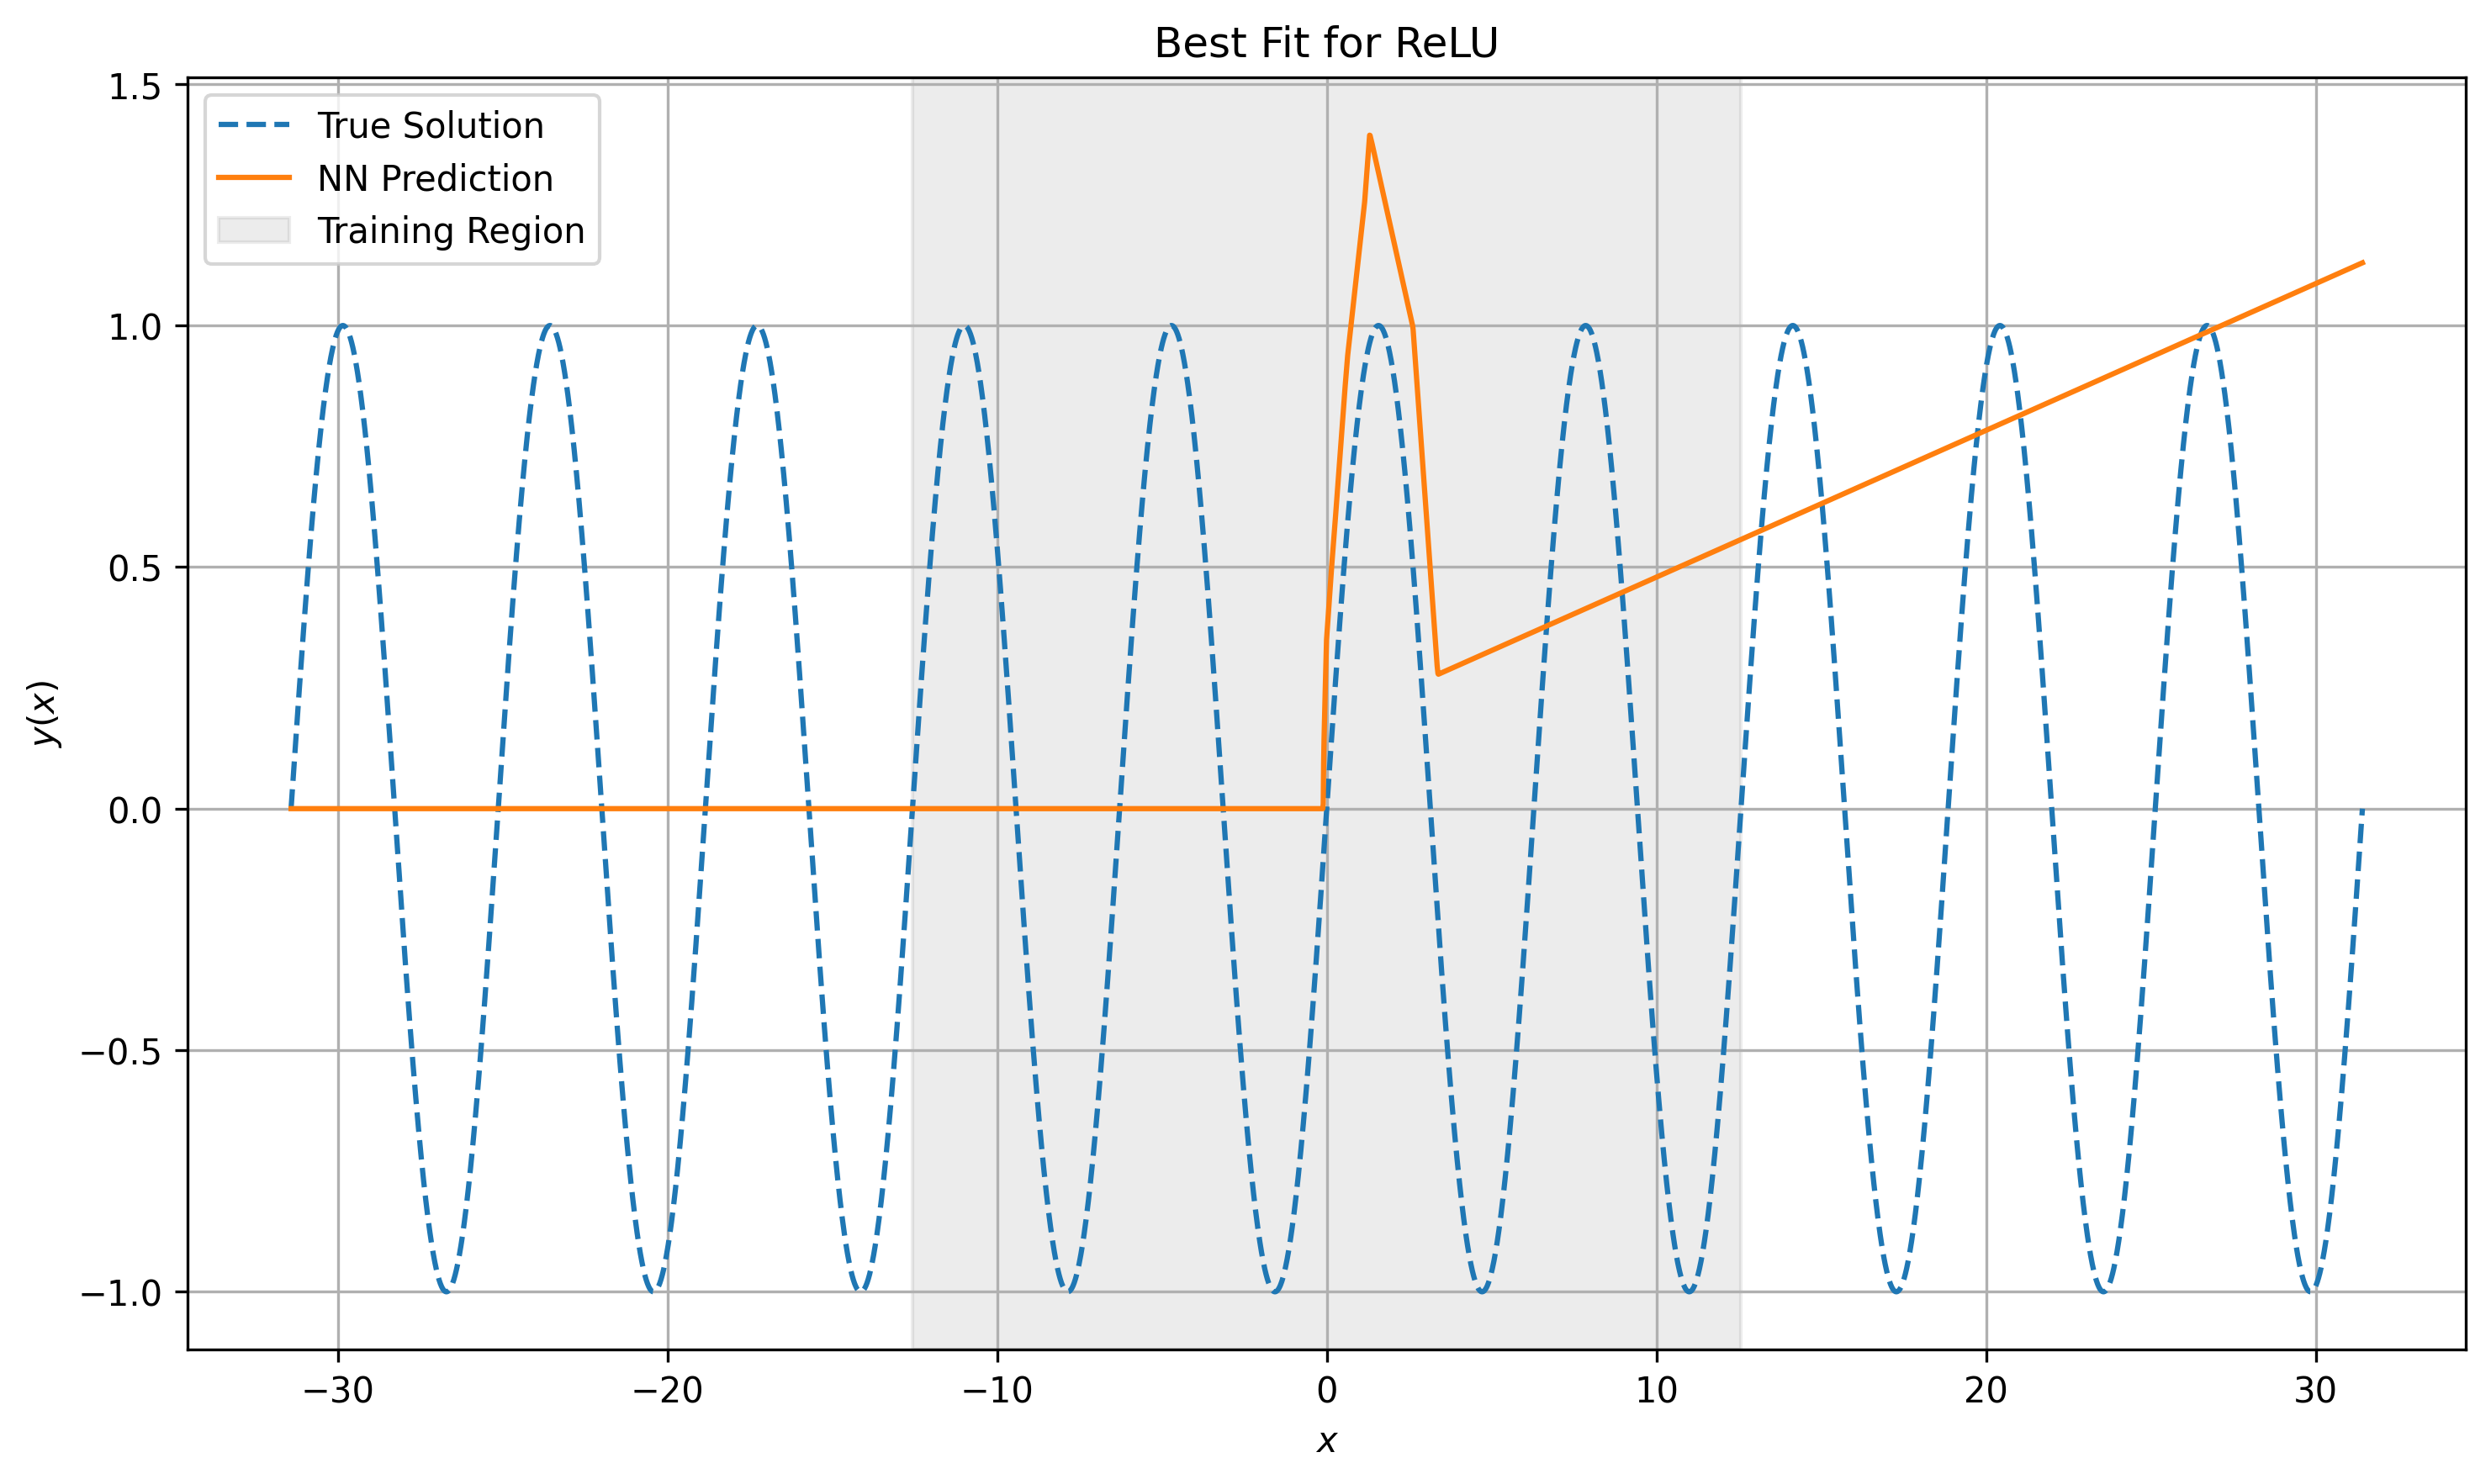
\includegraphics[width=\textwidth]{graphics/ivp_periodic_best_fit_relu_8layers_8width.png}
        \caption{\textbf{ReLU activation.} Heatmap (top), best fit (middle), and worst fit (bottom).}
        \label{fig:ivp_periodic_relu}
    \end{subfigure}
    \hspace*{\fill}
    \caption{Comparison of architectural performance for the exponential decay problem using two 
    activation functions. Each column shows the MSE heatmap with a log error scale,
    the best network fit, and the worst network fit.}
    \label{fig:ivp_periodic_sidebyside}
\end{figure}

We first observe that the neural networks using the $\tanh$ activation function are clearly more
successful at solving this particular solution, almost entirely failing to....


\paragraph{Singular Solution}

We now turn to an initial value problem whose solution contains a singularity:
\[
\begin{aligned}
    y'(x) &= y(x)^2, \\
    y(0) &= 1, \\
    y(1.05) &= -20
\end{aligned}
\]
The exact solution is \( y(x) = \frac{1}{1 - x} \), which becomes singular at \( x = 1 \). This 
problem is useful for testing the ability of neural networks to approximate rapidly varying functions 
and to capture solution blow-up within a finite domain.

To mitigate instability near the singularity, we train two separate networks: one on the interval 
\([0, 0.95]\) using the initial condition \( y(0) = 1 \), and one on the interval \([1.05, 2.0] \) 
using the analytically derived condition \( y(1.05) = -20 \). This approach allows us to evaluate how 
well neural networks can approximate the solution on either side of the singularity without 
numerical breakdown.

\begin{figure}[h]
    \centering
    \hspace*{\fill}
    \begin{subfigure}[t]{0.48\textwidth}
        \centering
        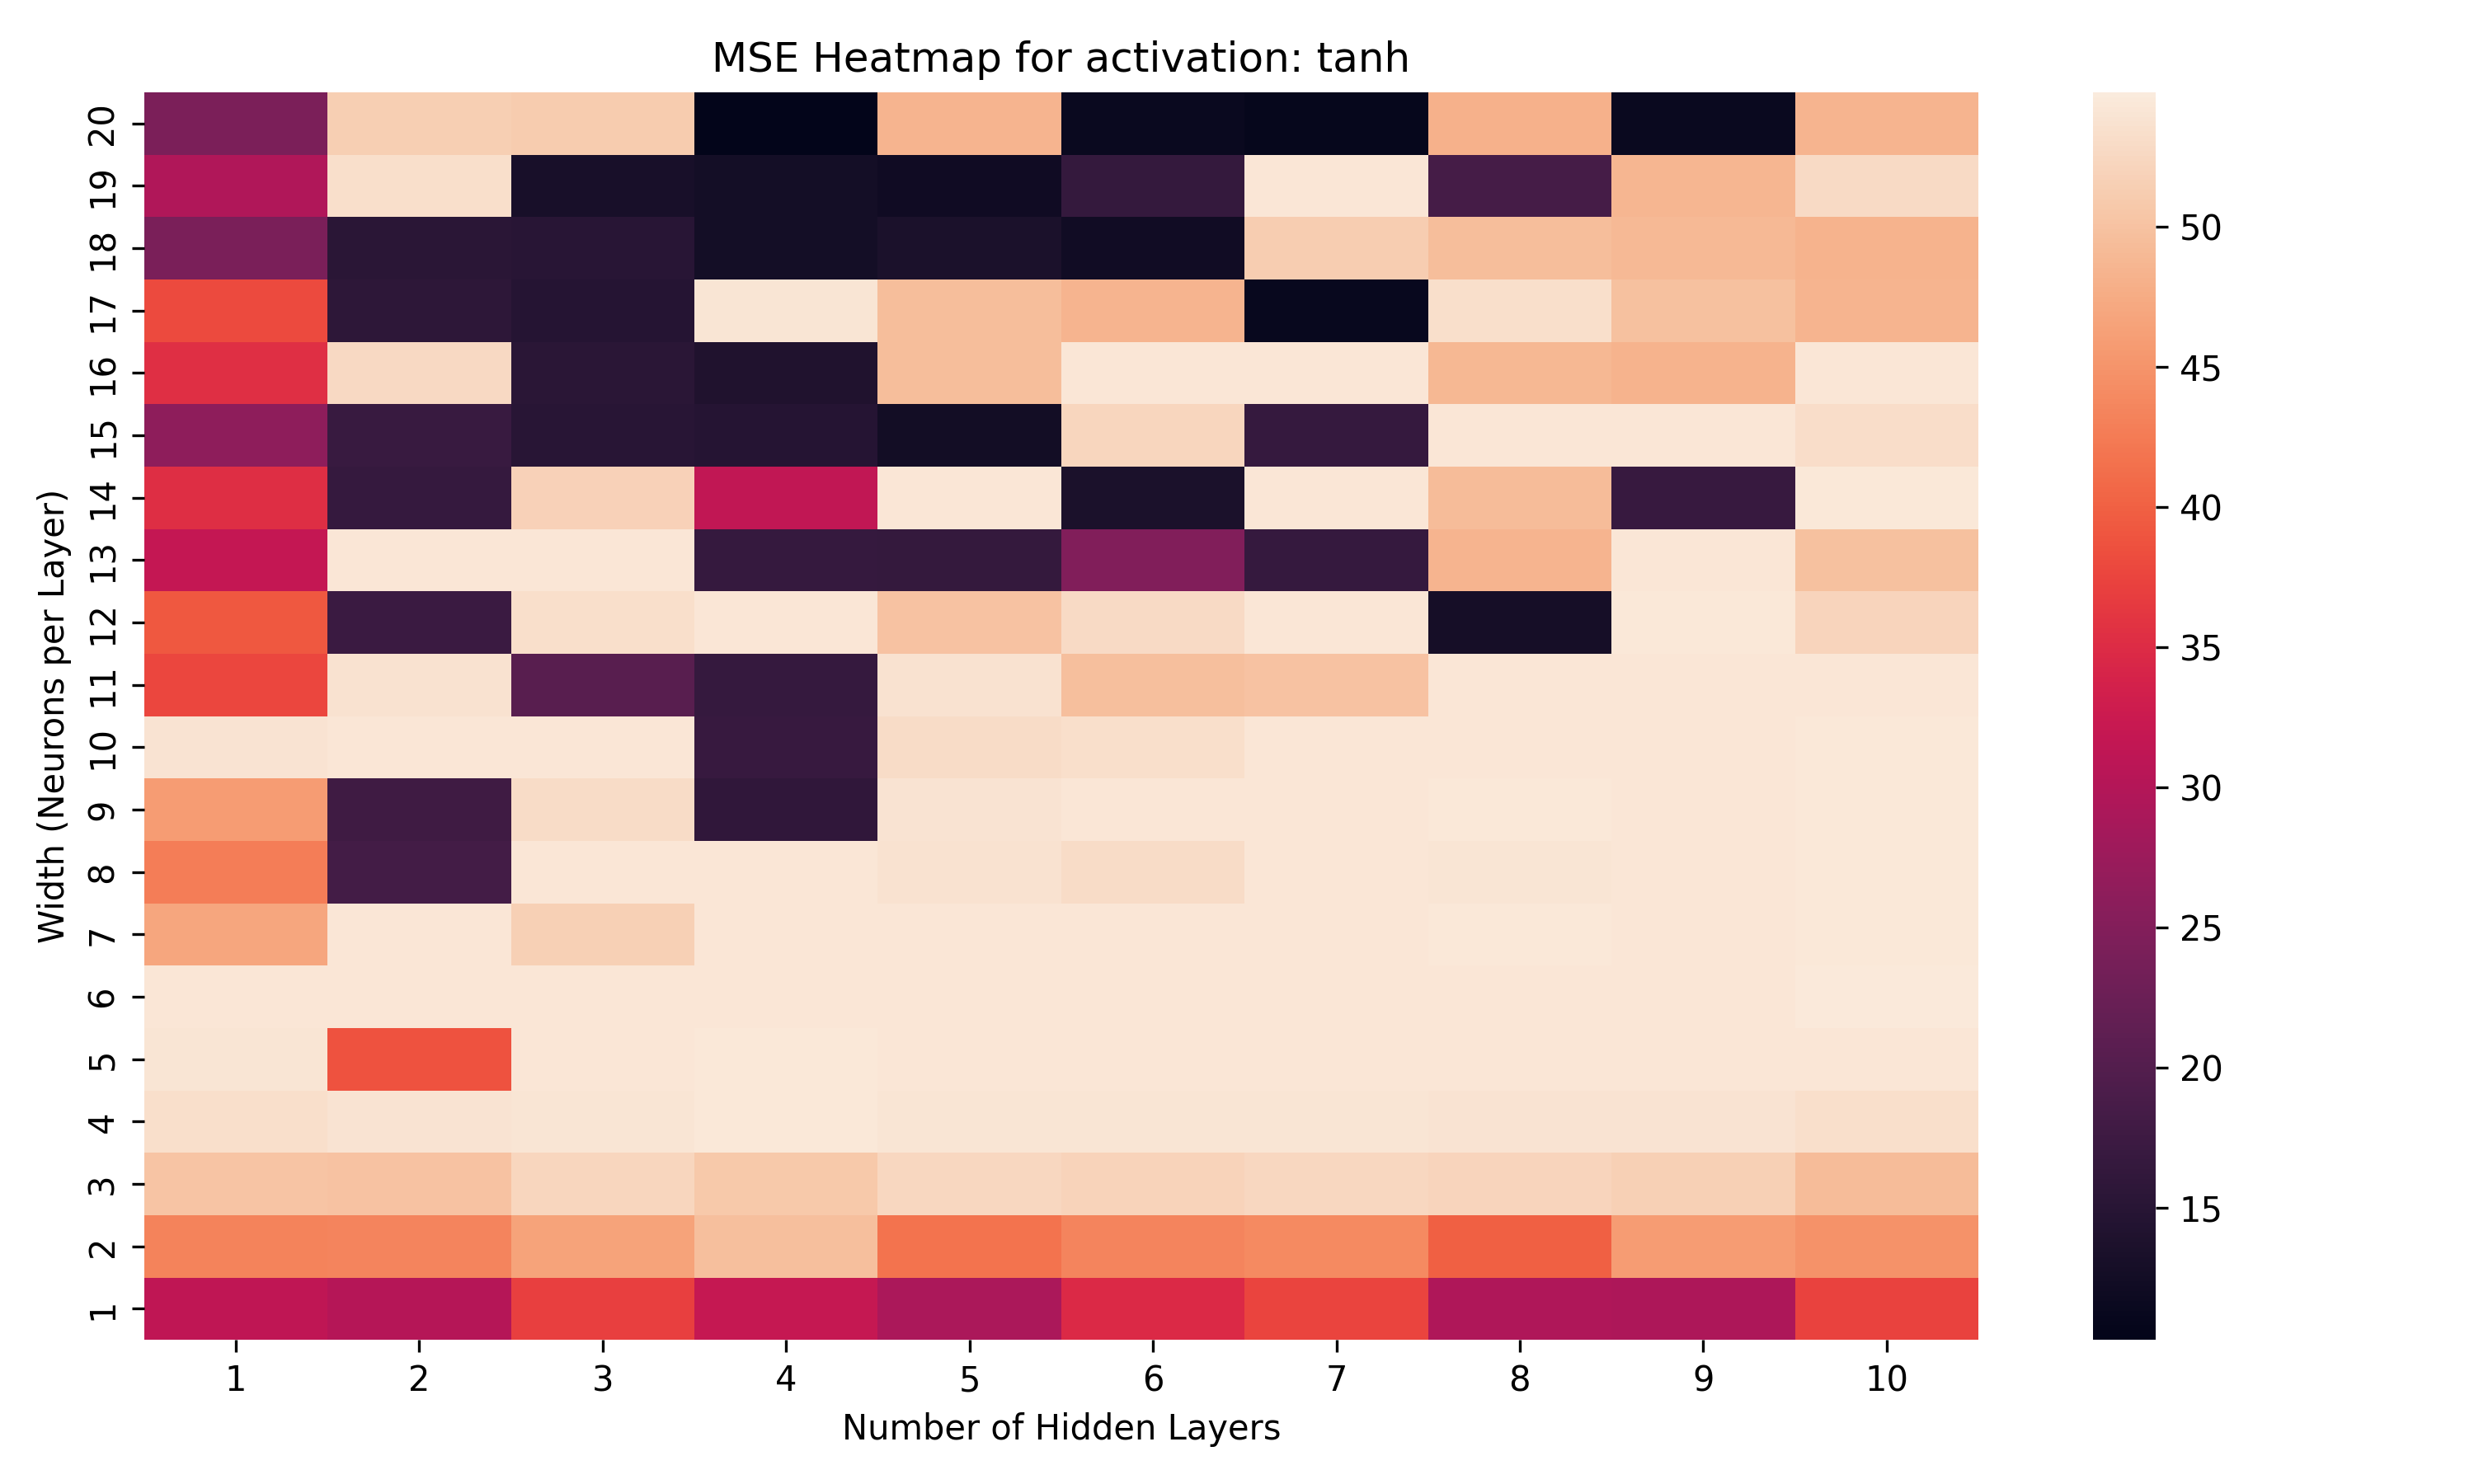
\includegraphics[width=\textwidth]{graphics/mse_heatmap_ivp_singularity_tanh.png}
        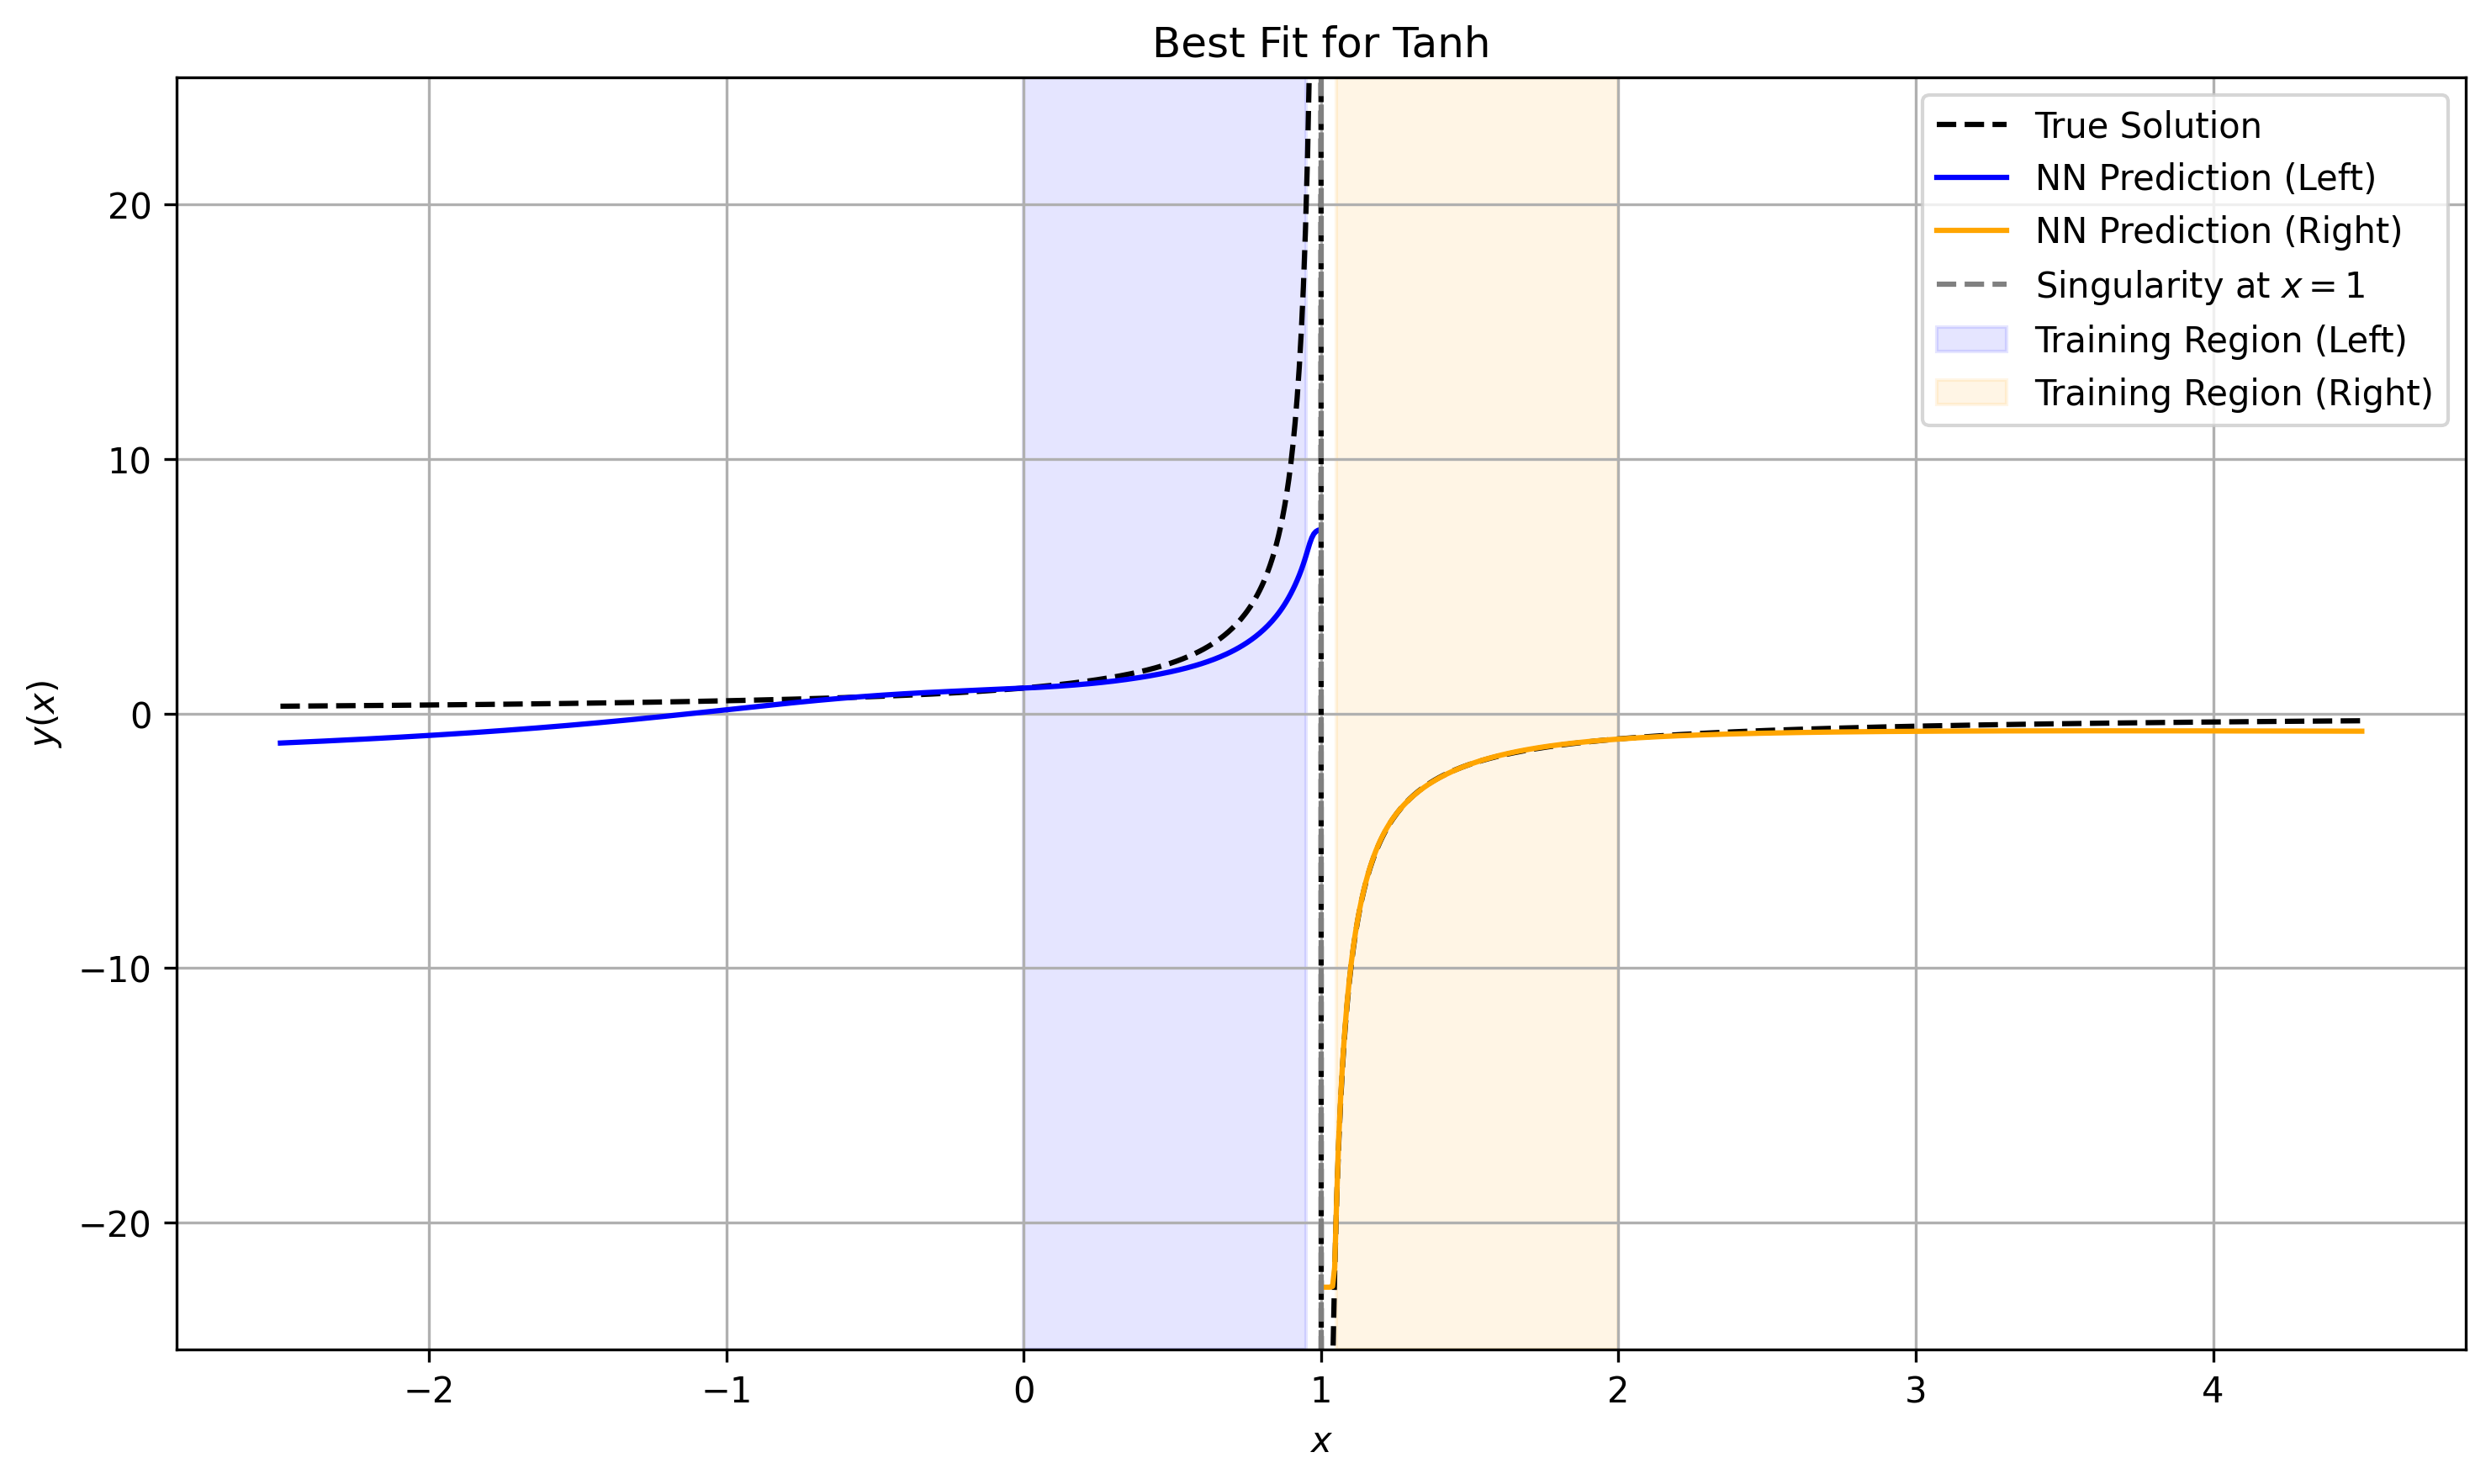
\includegraphics[width=\textwidth]{graphics/ivp_singularity_best_fit_tanh_7layers_15width.png}
        \caption{\textbf{Tanh activation.} Heatmap (top), best fit (middle), and worst fit (bottom).}
        \label{fig:ivp_periodic_tanh}
    \end{subfigure}
    \hspace*{\fill}
    \begin{subfigure}[t]{0.48\textwidth}
        \centering
        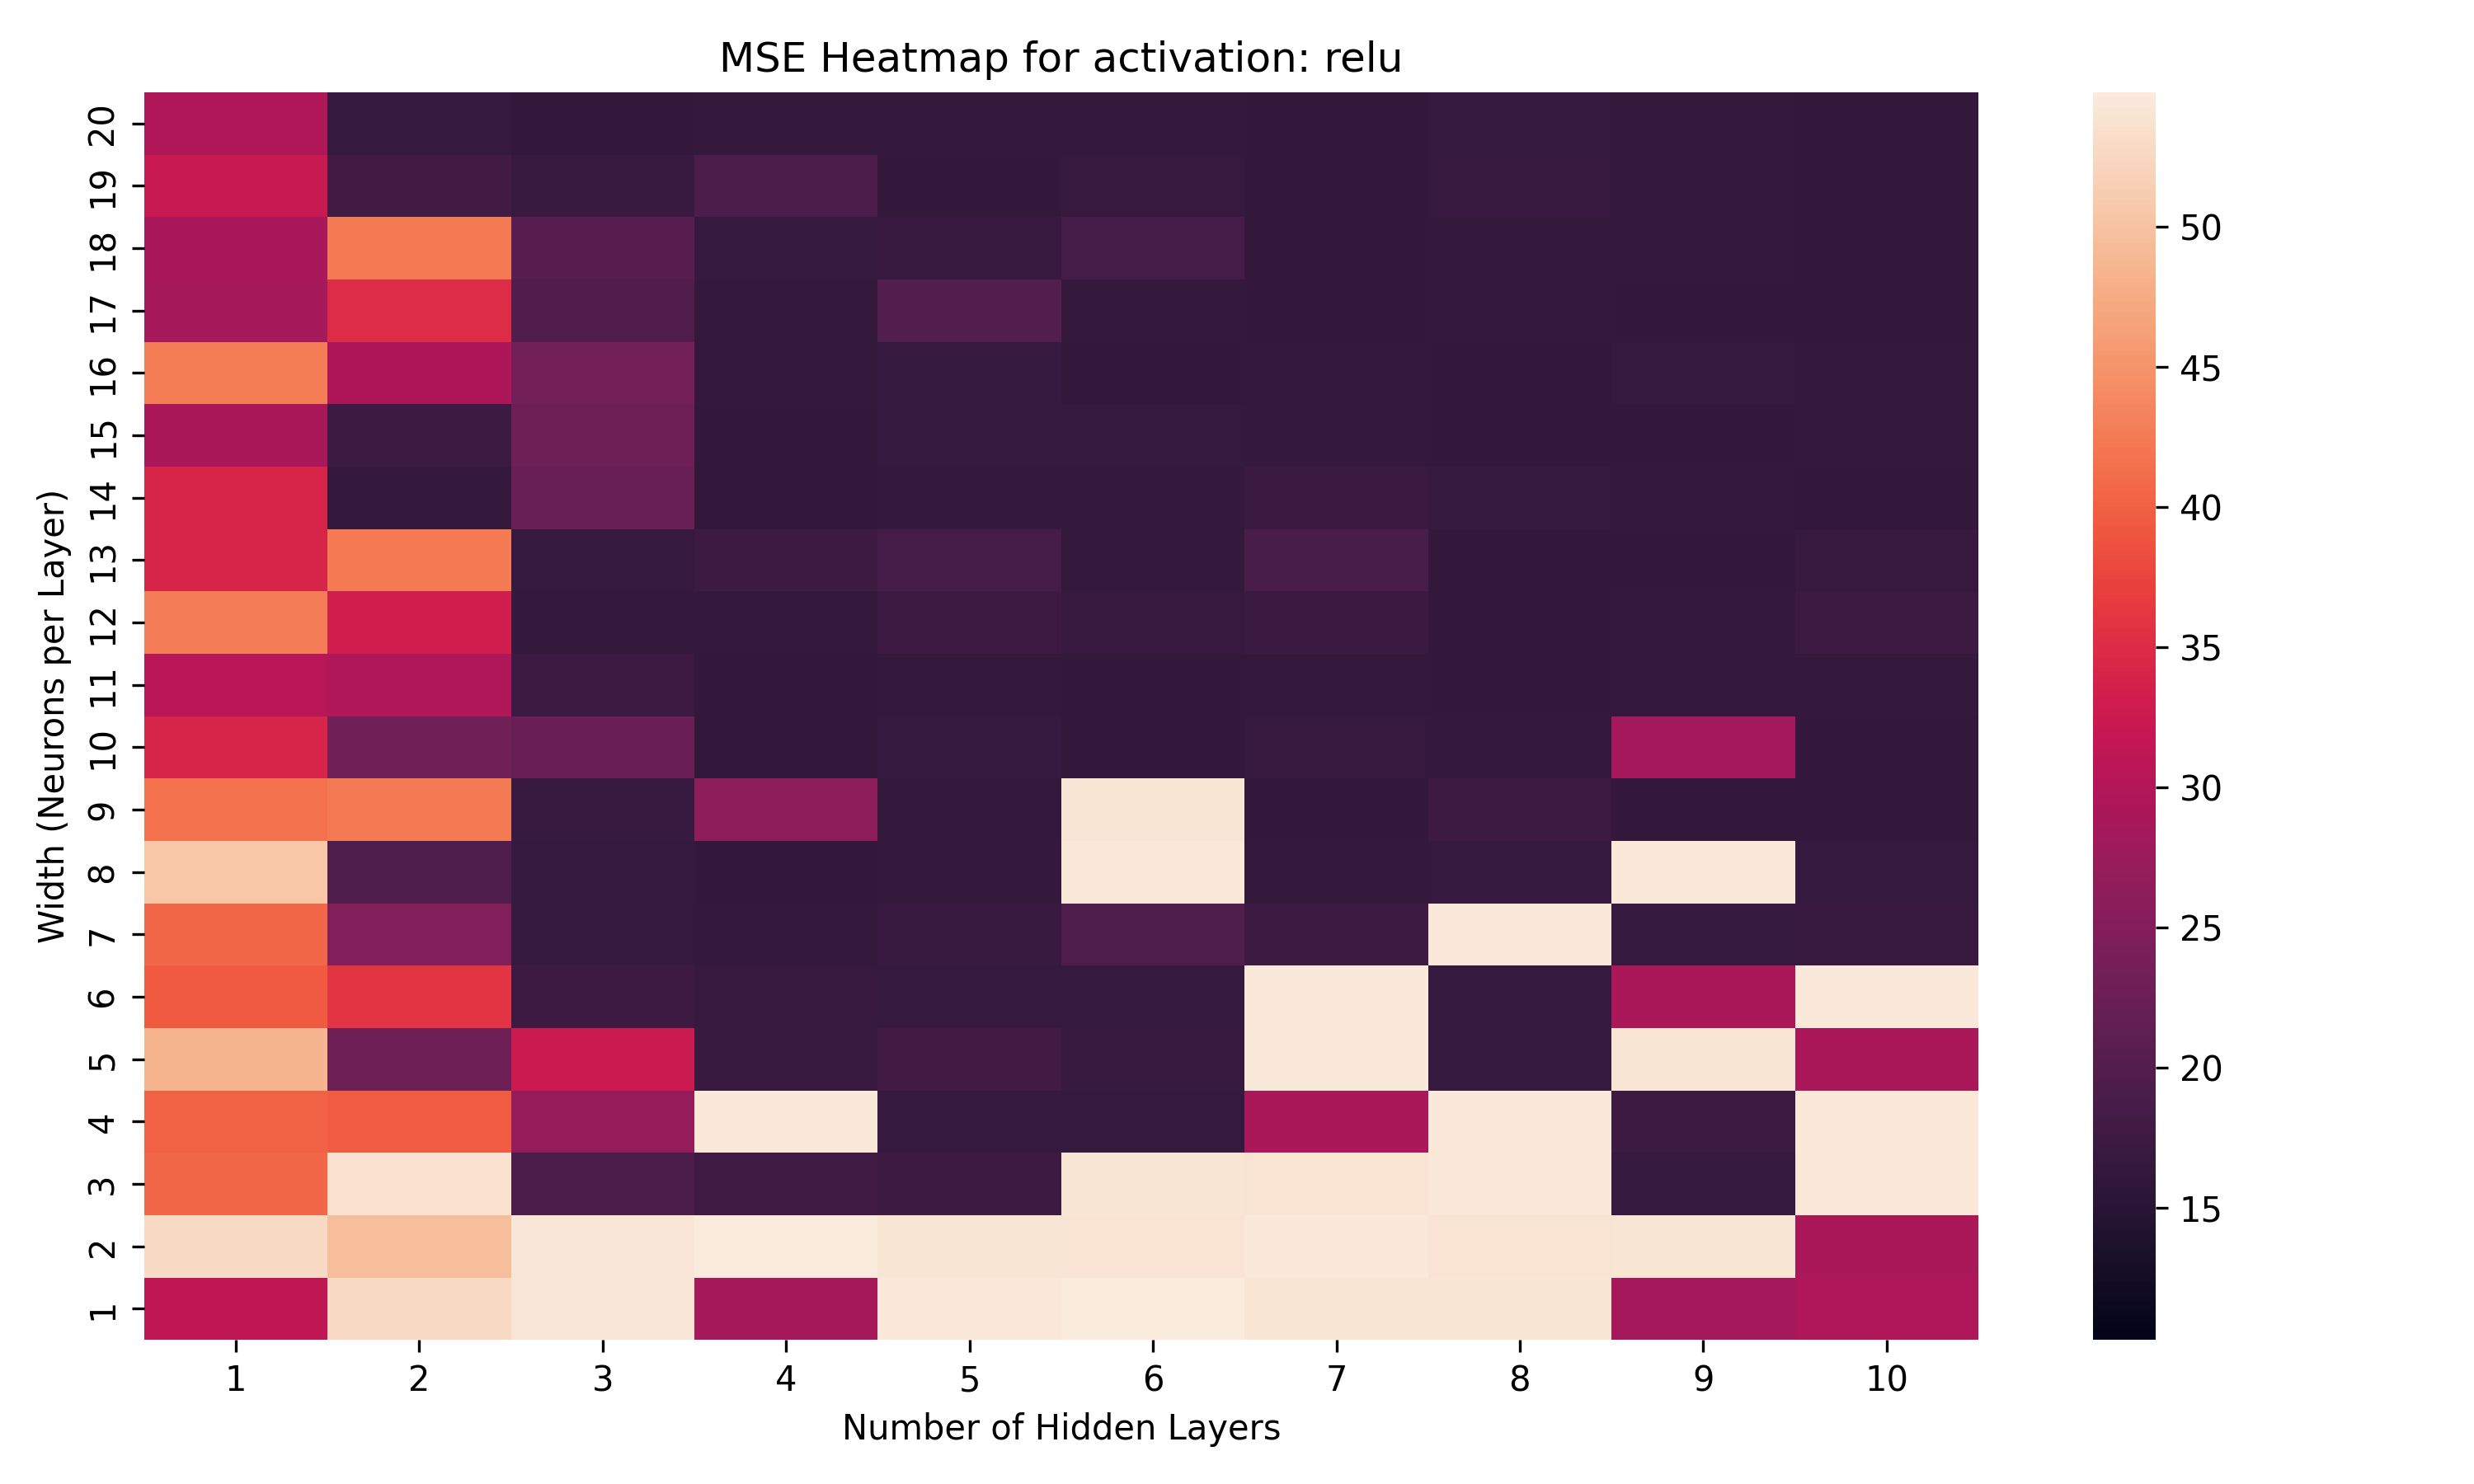
\includegraphics[width=\textwidth]{graphics/mse_heatmap_ivp_singularity_relu.png}
        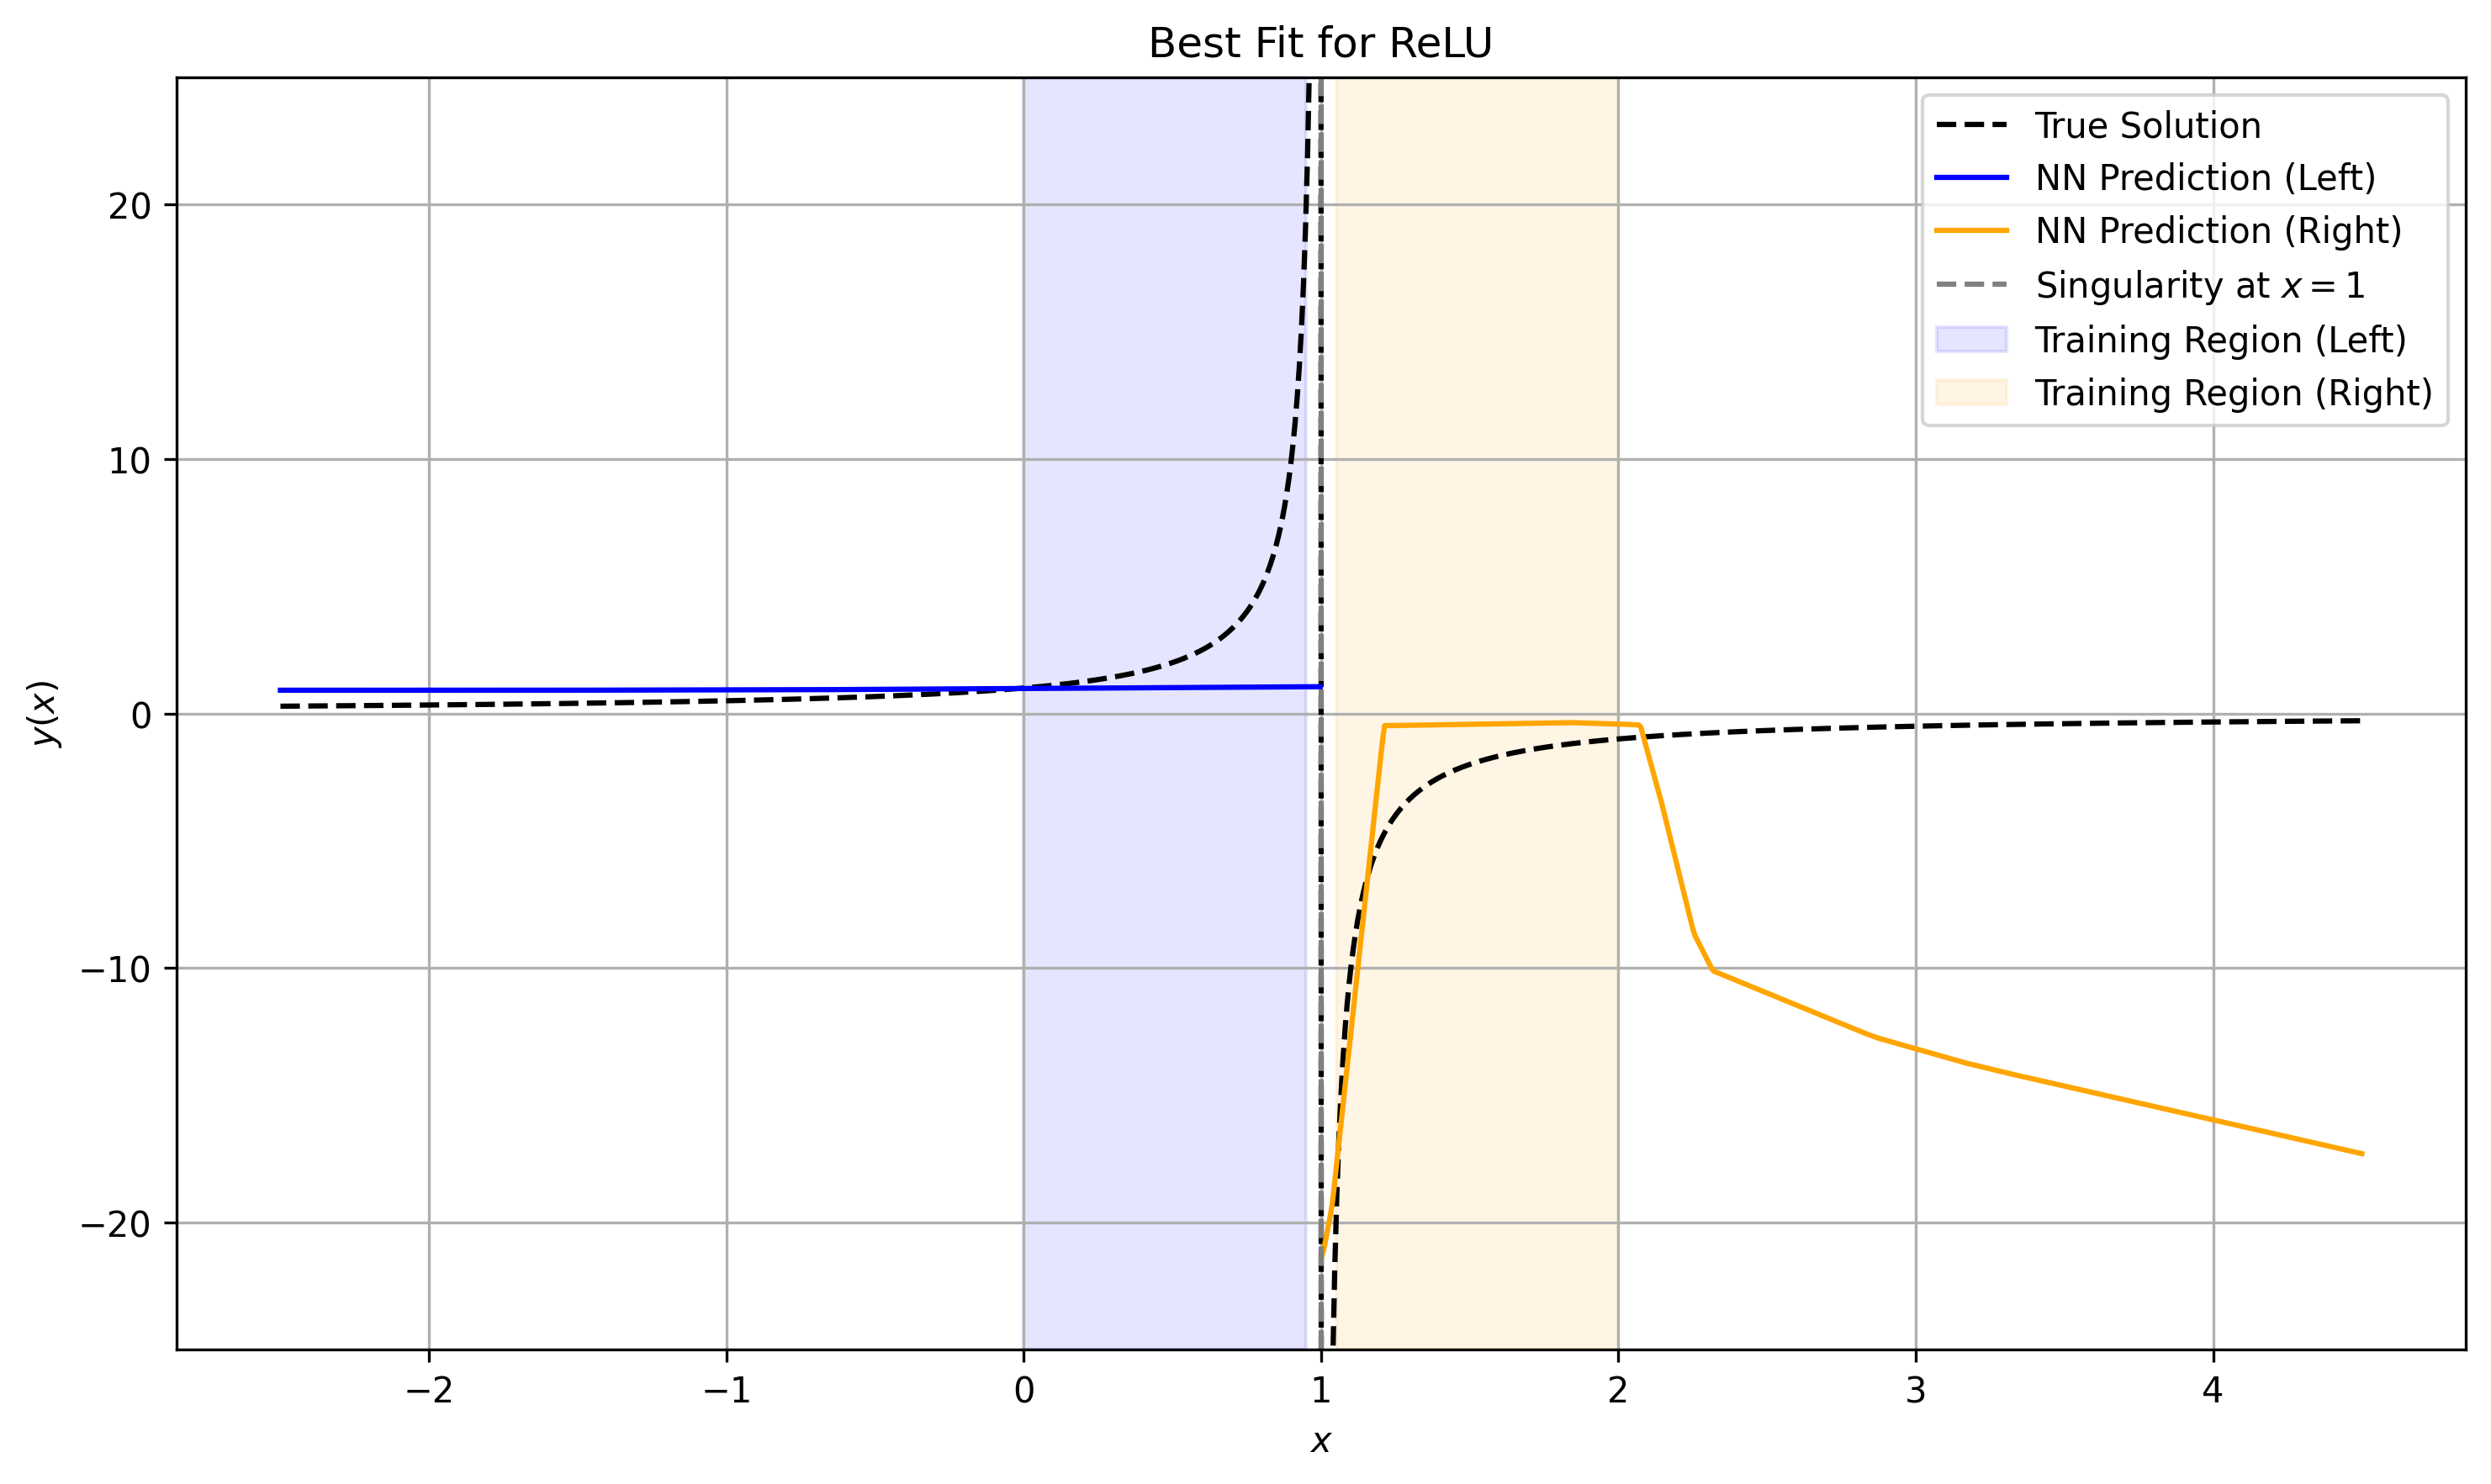
\includegraphics[width=\textwidth]{graphics/ivp_singularity_best_fit_relu_8layers_8width.png}
        \caption{\textbf{ReLU activation.} Heatmap (top), best fit (middle), and worst fit (bottom).}
        \label{fig:ivp_periodic_relu}
    \end{subfigure}
    \hspace*{\fill}
    \caption{Comparison of architectural performance for the exponential decay problem using two 
    activation functions. Each column shows the MSE heatmap with a log error scale,
    the best network fit, and the worst network fit.}
    \label{fig:ivp_periodic_sidebyside}
\end{figure}



\subsection{Boundary Value Problems}\label{sec:BVPs}


We now consider boundary value problems (BVPs), where the solution is defined by a 
differential equation along with prescribed values at the boundaries of a fixed domain. Unlike 
initial value problems, BVPs specify constraints at multiple points—typically at the endpoints of 
an interval—and the solution must satisfy the differential equation throughout the domain while 
adhering to these boundary conditions.

In this section, we investigate how well neural networks can approximate solutions to BVPs using 
the same methodology outlined for IVPs. However, since BVPs are defined strictly on a bounded 
interval, we do not consider extrapolation performance here. Instead, we focus on how accurately 
the networks capture the solution within the specified domain.

We consider two representative BVPs:
\begin{itemize}
    \item A smooth Poisson-type problem, with known analytic solution $y(x)=sin(\pi x)$, 
    serving as a baseline. 
    \item A piecewise forcing problem with a discontinuous right-hand side, used to examine network
     behaviour under more challenging conditions. 
\end{itemize}

For each problem, we evaluate neural network performance across a range of architectures and 
activation functions, using mean squared error (MSE) as the primary metric. Heatmaps and example 
fits are used to visualise how architectural choices affect solution quality.



\paragraph{Poisson Problem}

We begin with a classical boundary value problem from mathematical physics:
\[
\begin{aligned}
    -y''(x) &= \pi^2 \sin(\pi x), \quad x \in (0, 1), \\
    y(0) &= 0, \\
    y(1) &= 0.
\end{aligned}
\]
This has the exact solution \( y(x) = \sin(\pi x) \), which is smooth, bounded, and vanishes at both 
endpoints.  
The problem provides a simple but instructive setting to evaluate how well neural networks approximate 
solutions to second-order differential equations with smooth forcing and well-defined boundary 
conditions.

As in the IVP analysis, we assess the effect of architectural variation on solution accuracy.
For each combination of depth, width, and activation function, we compute the MSE across the domain,
and visualise the results using heatmaps and representative fits. The best solutions are shown in 
Figure~\ref{fig:bvp_poisson_sidebyside}.

\begin{figure}[h]
    \centering
    \hspace*{\fill}
    \begin{subfigure}[t]{0.48\textwidth}
        \centering
        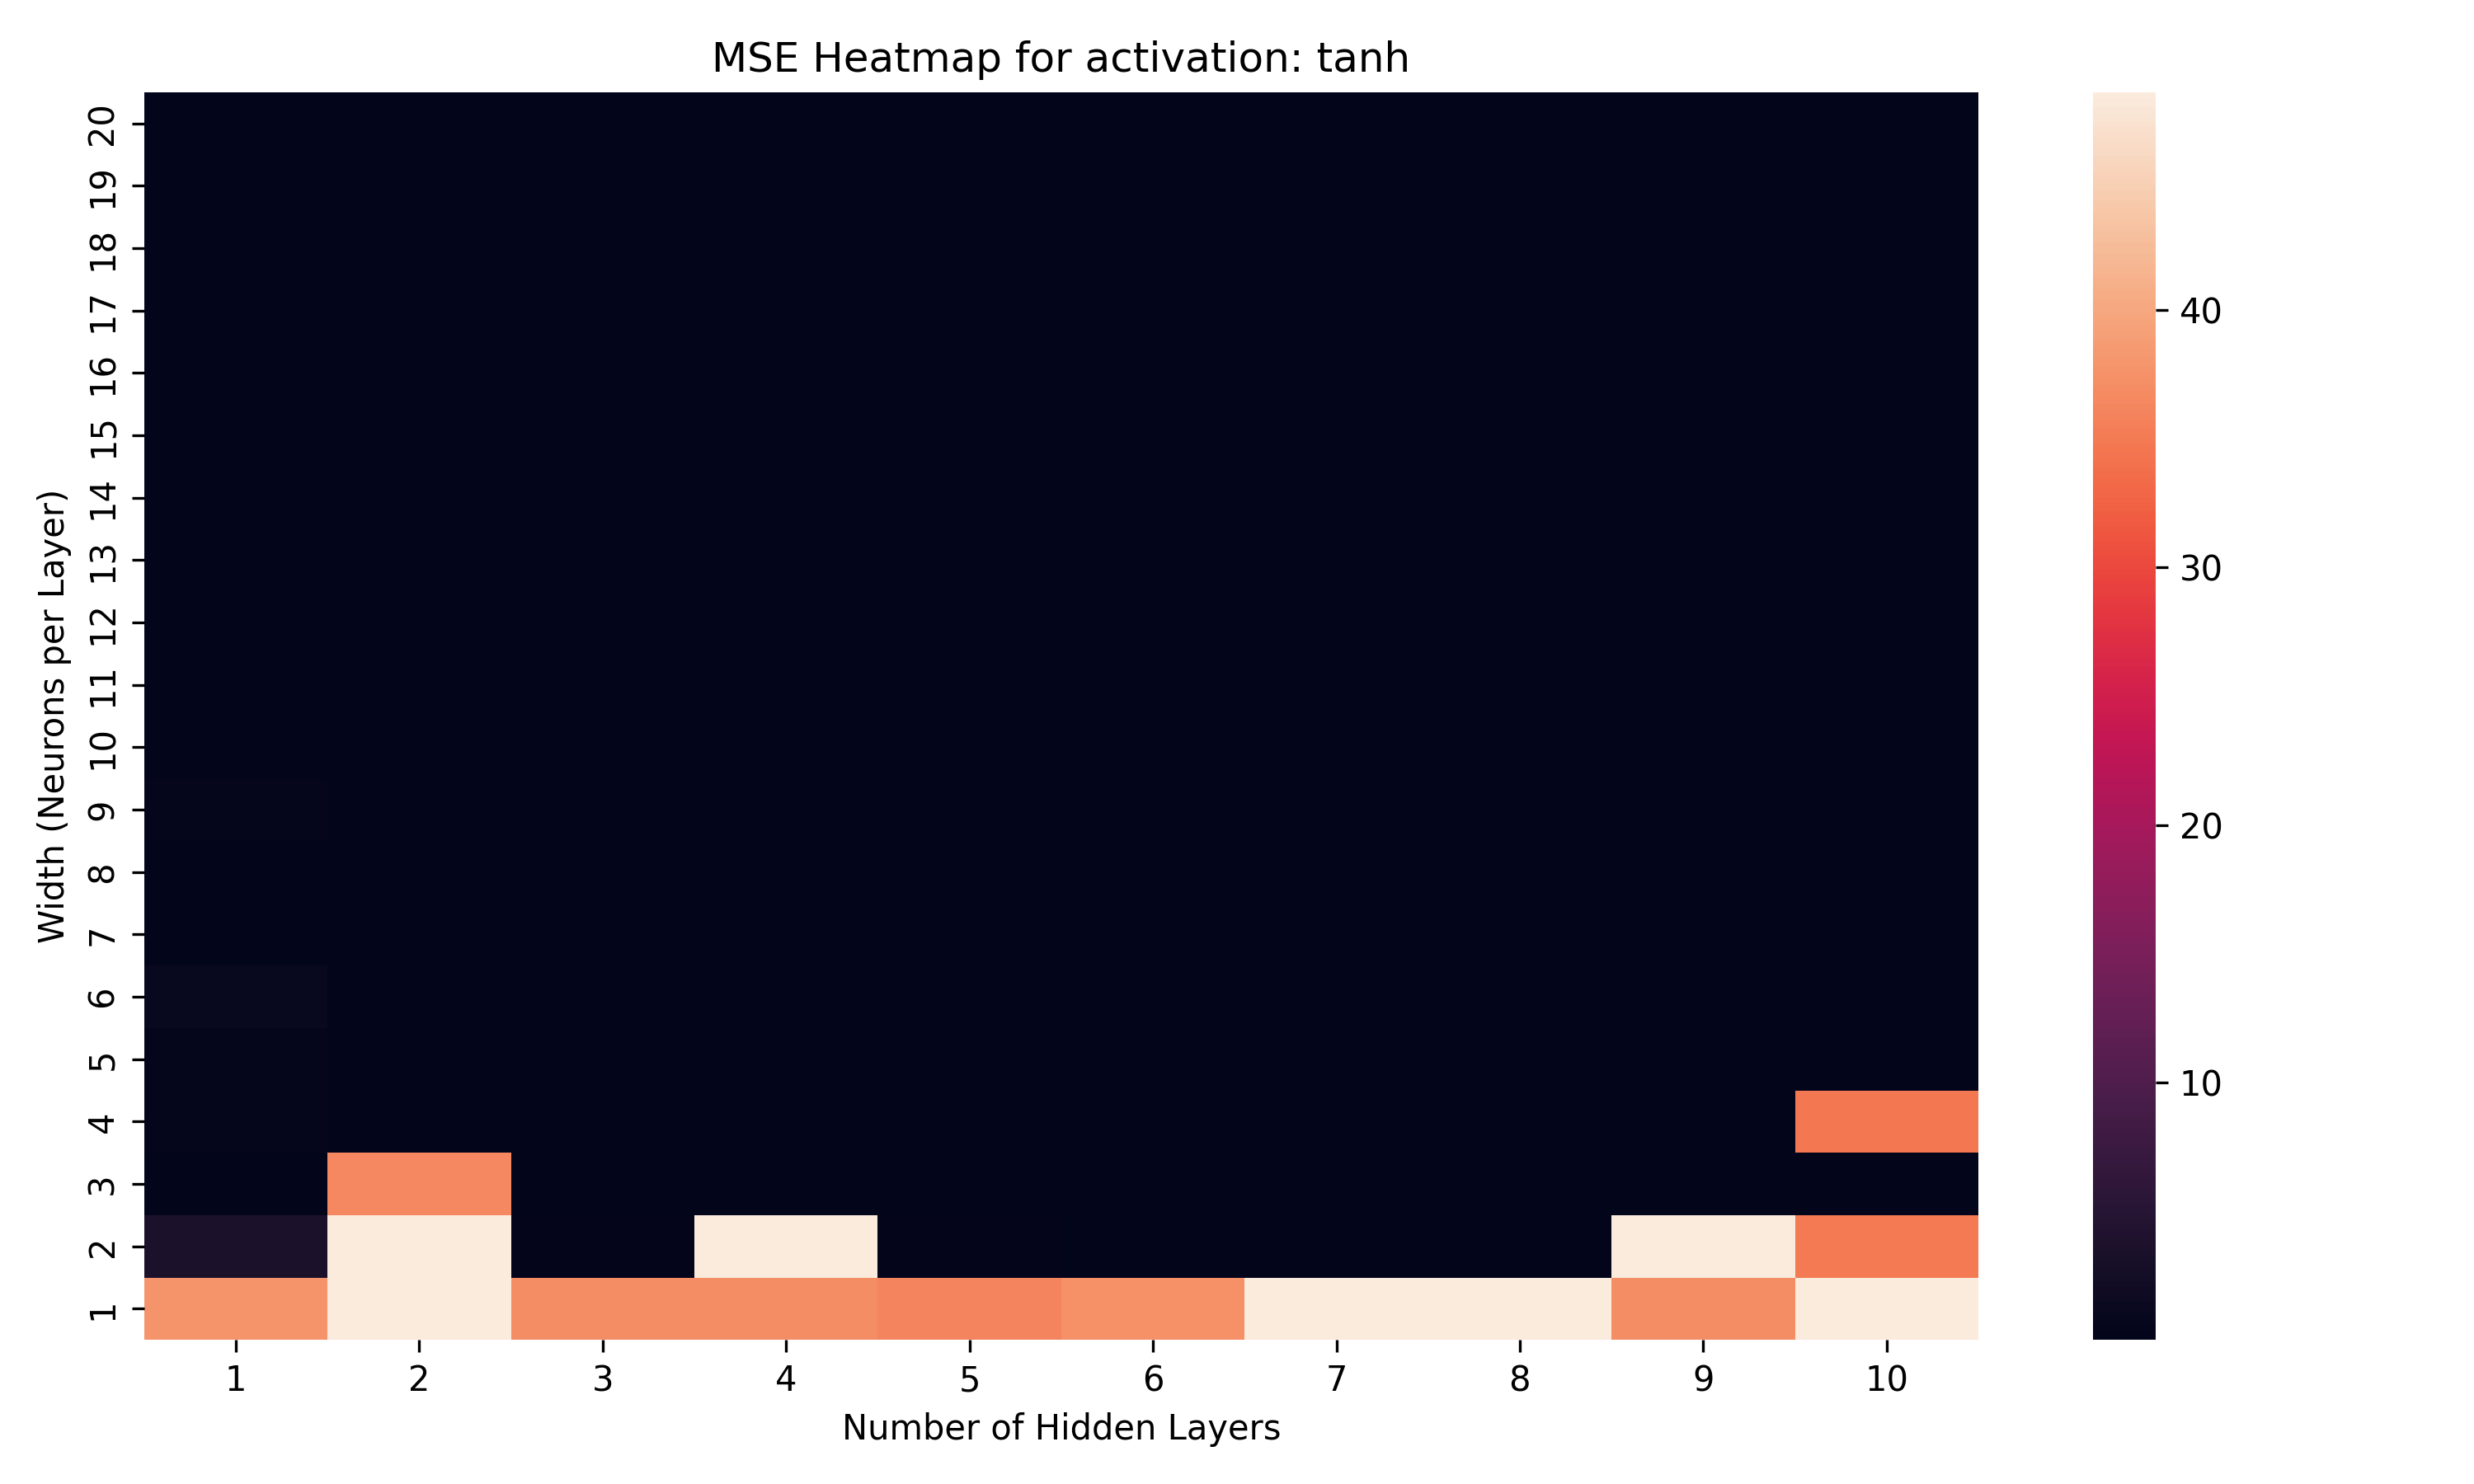
\includegraphics[width=\textwidth]{graphics/mse_heatmap_bvp_poisson_tanh.png}
        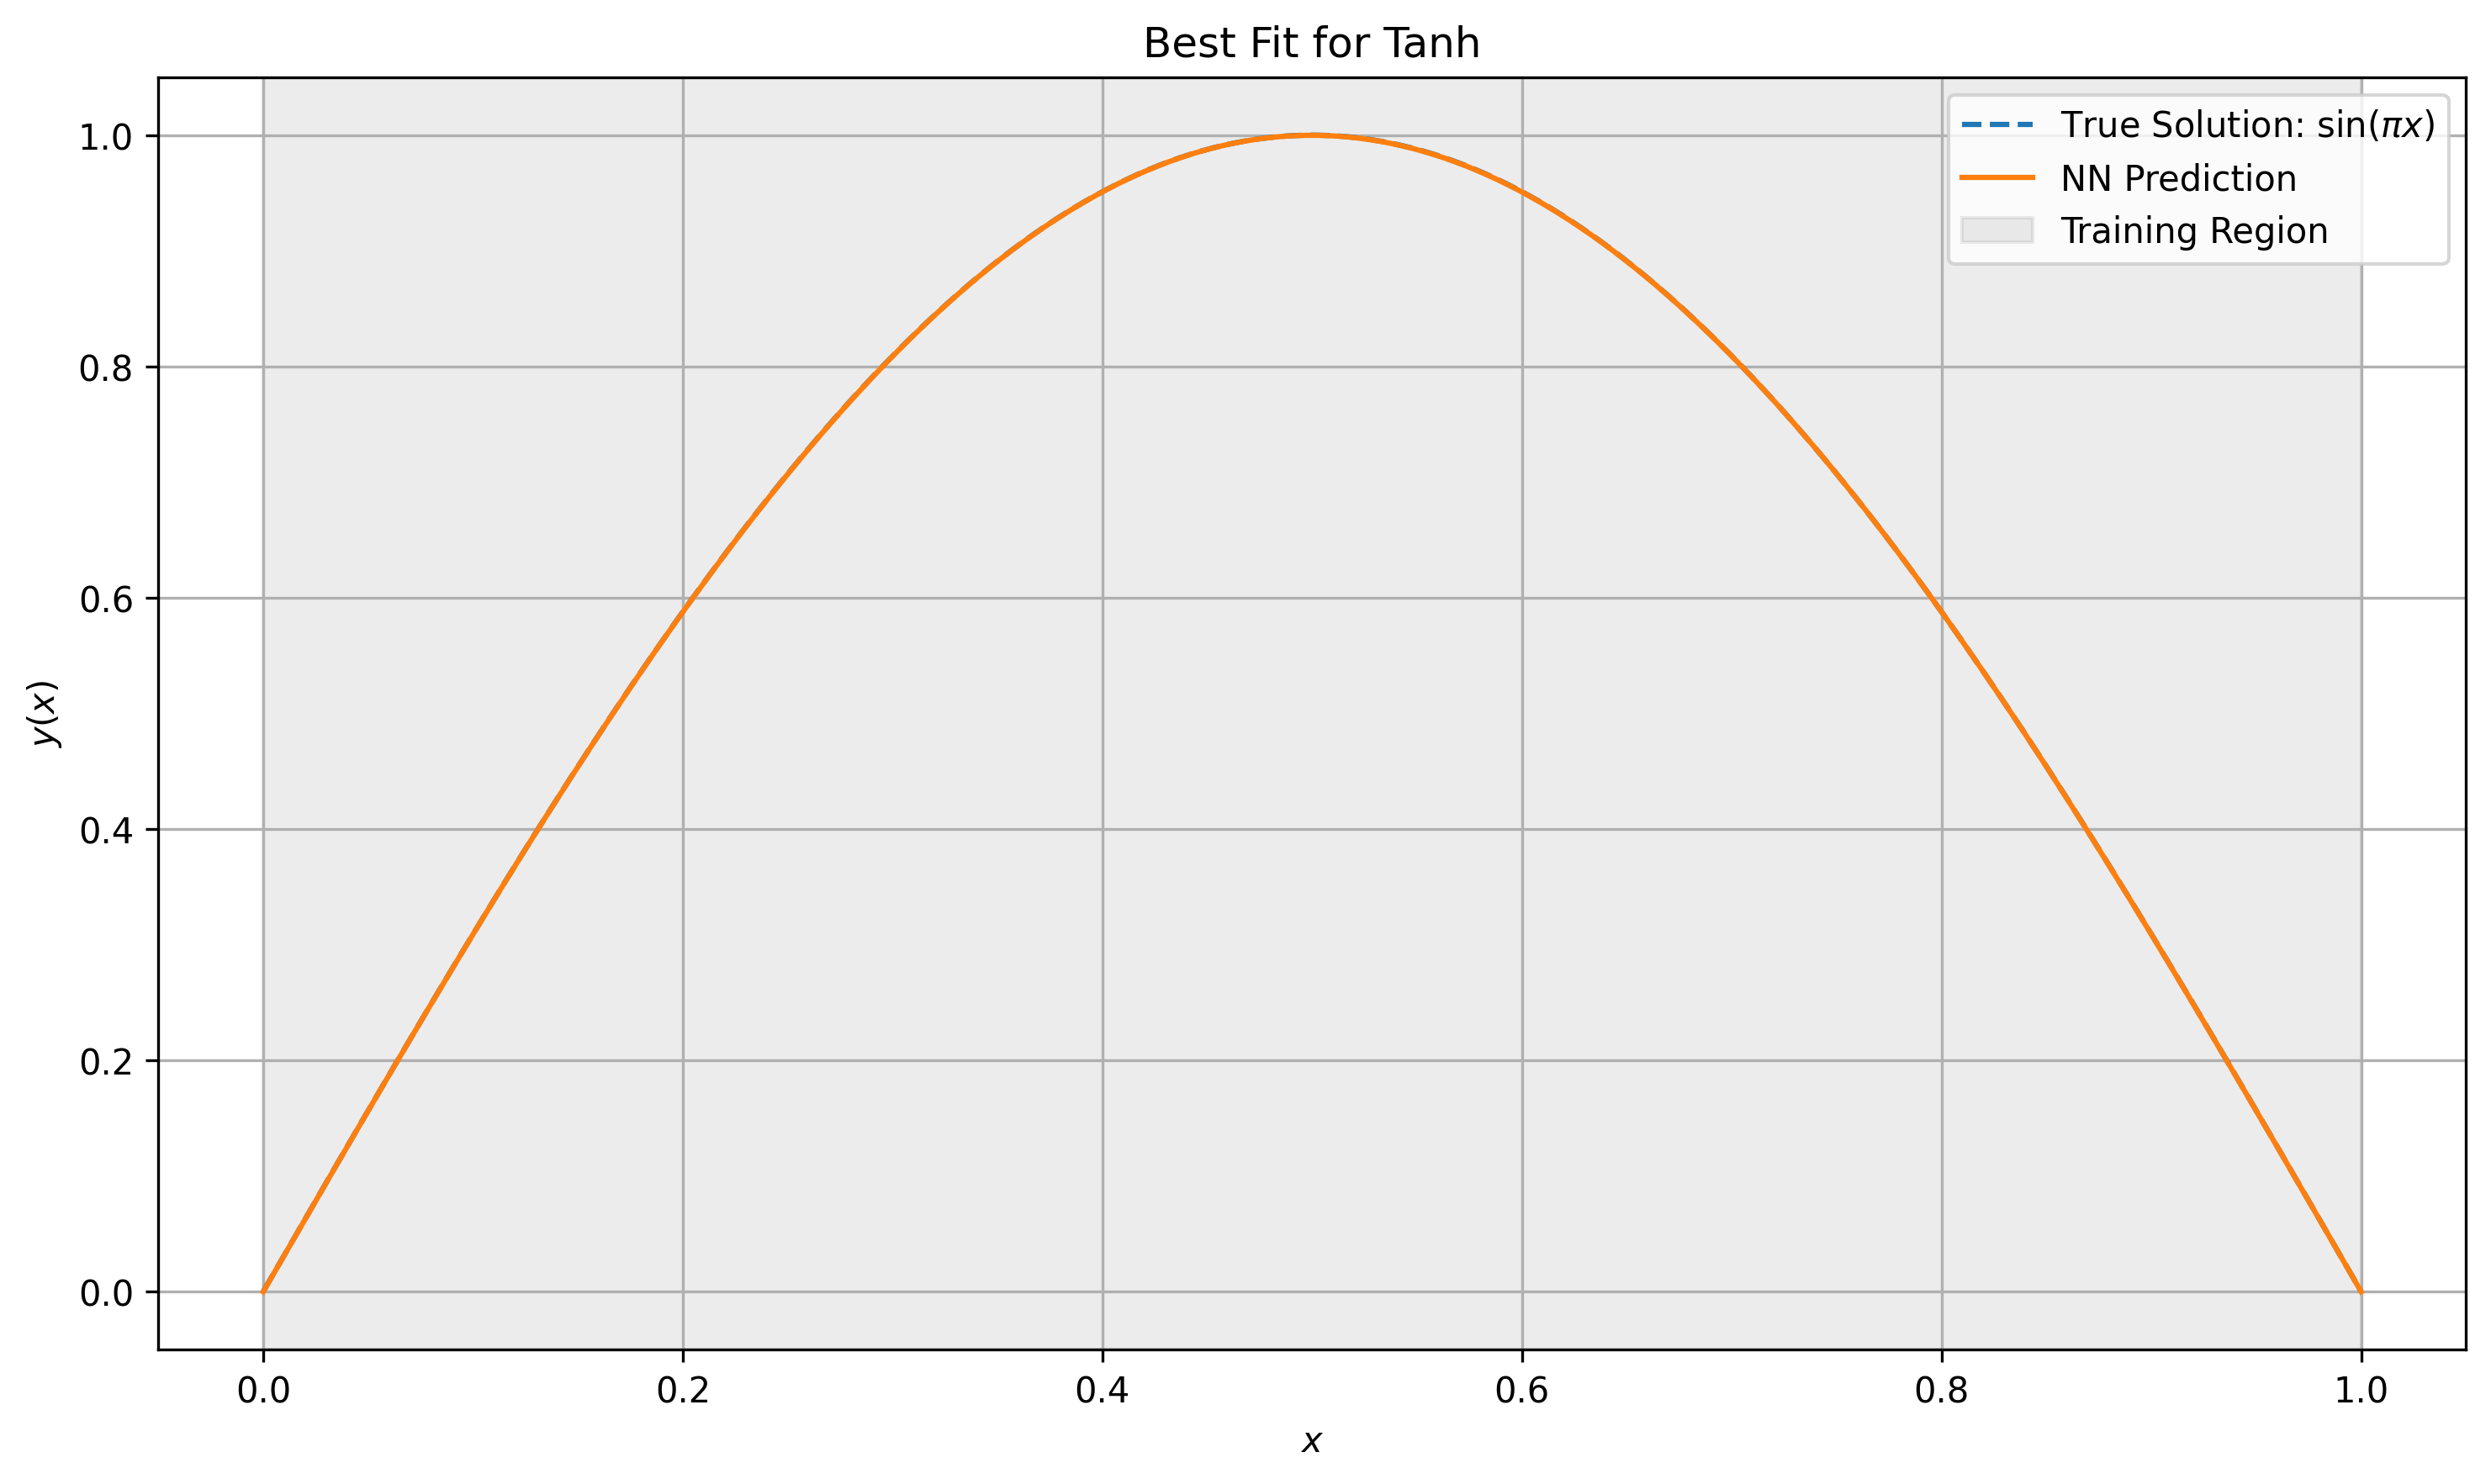
\includegraphics[width=\textwidth]{graphics/bvp_poisson_best_fit_tanh_9layers_18width.png}
        \caption{\textbf{Tanh activation.} Heatmap (top), best fit (middle), and worst fit (bottom).}
        \label{fig:ivp_periodic_tanh}
    \end{subfigure}
    \hspace*{\fill}
    \begin{subfigure}[t]{0.48\textwidth}
        \centering
        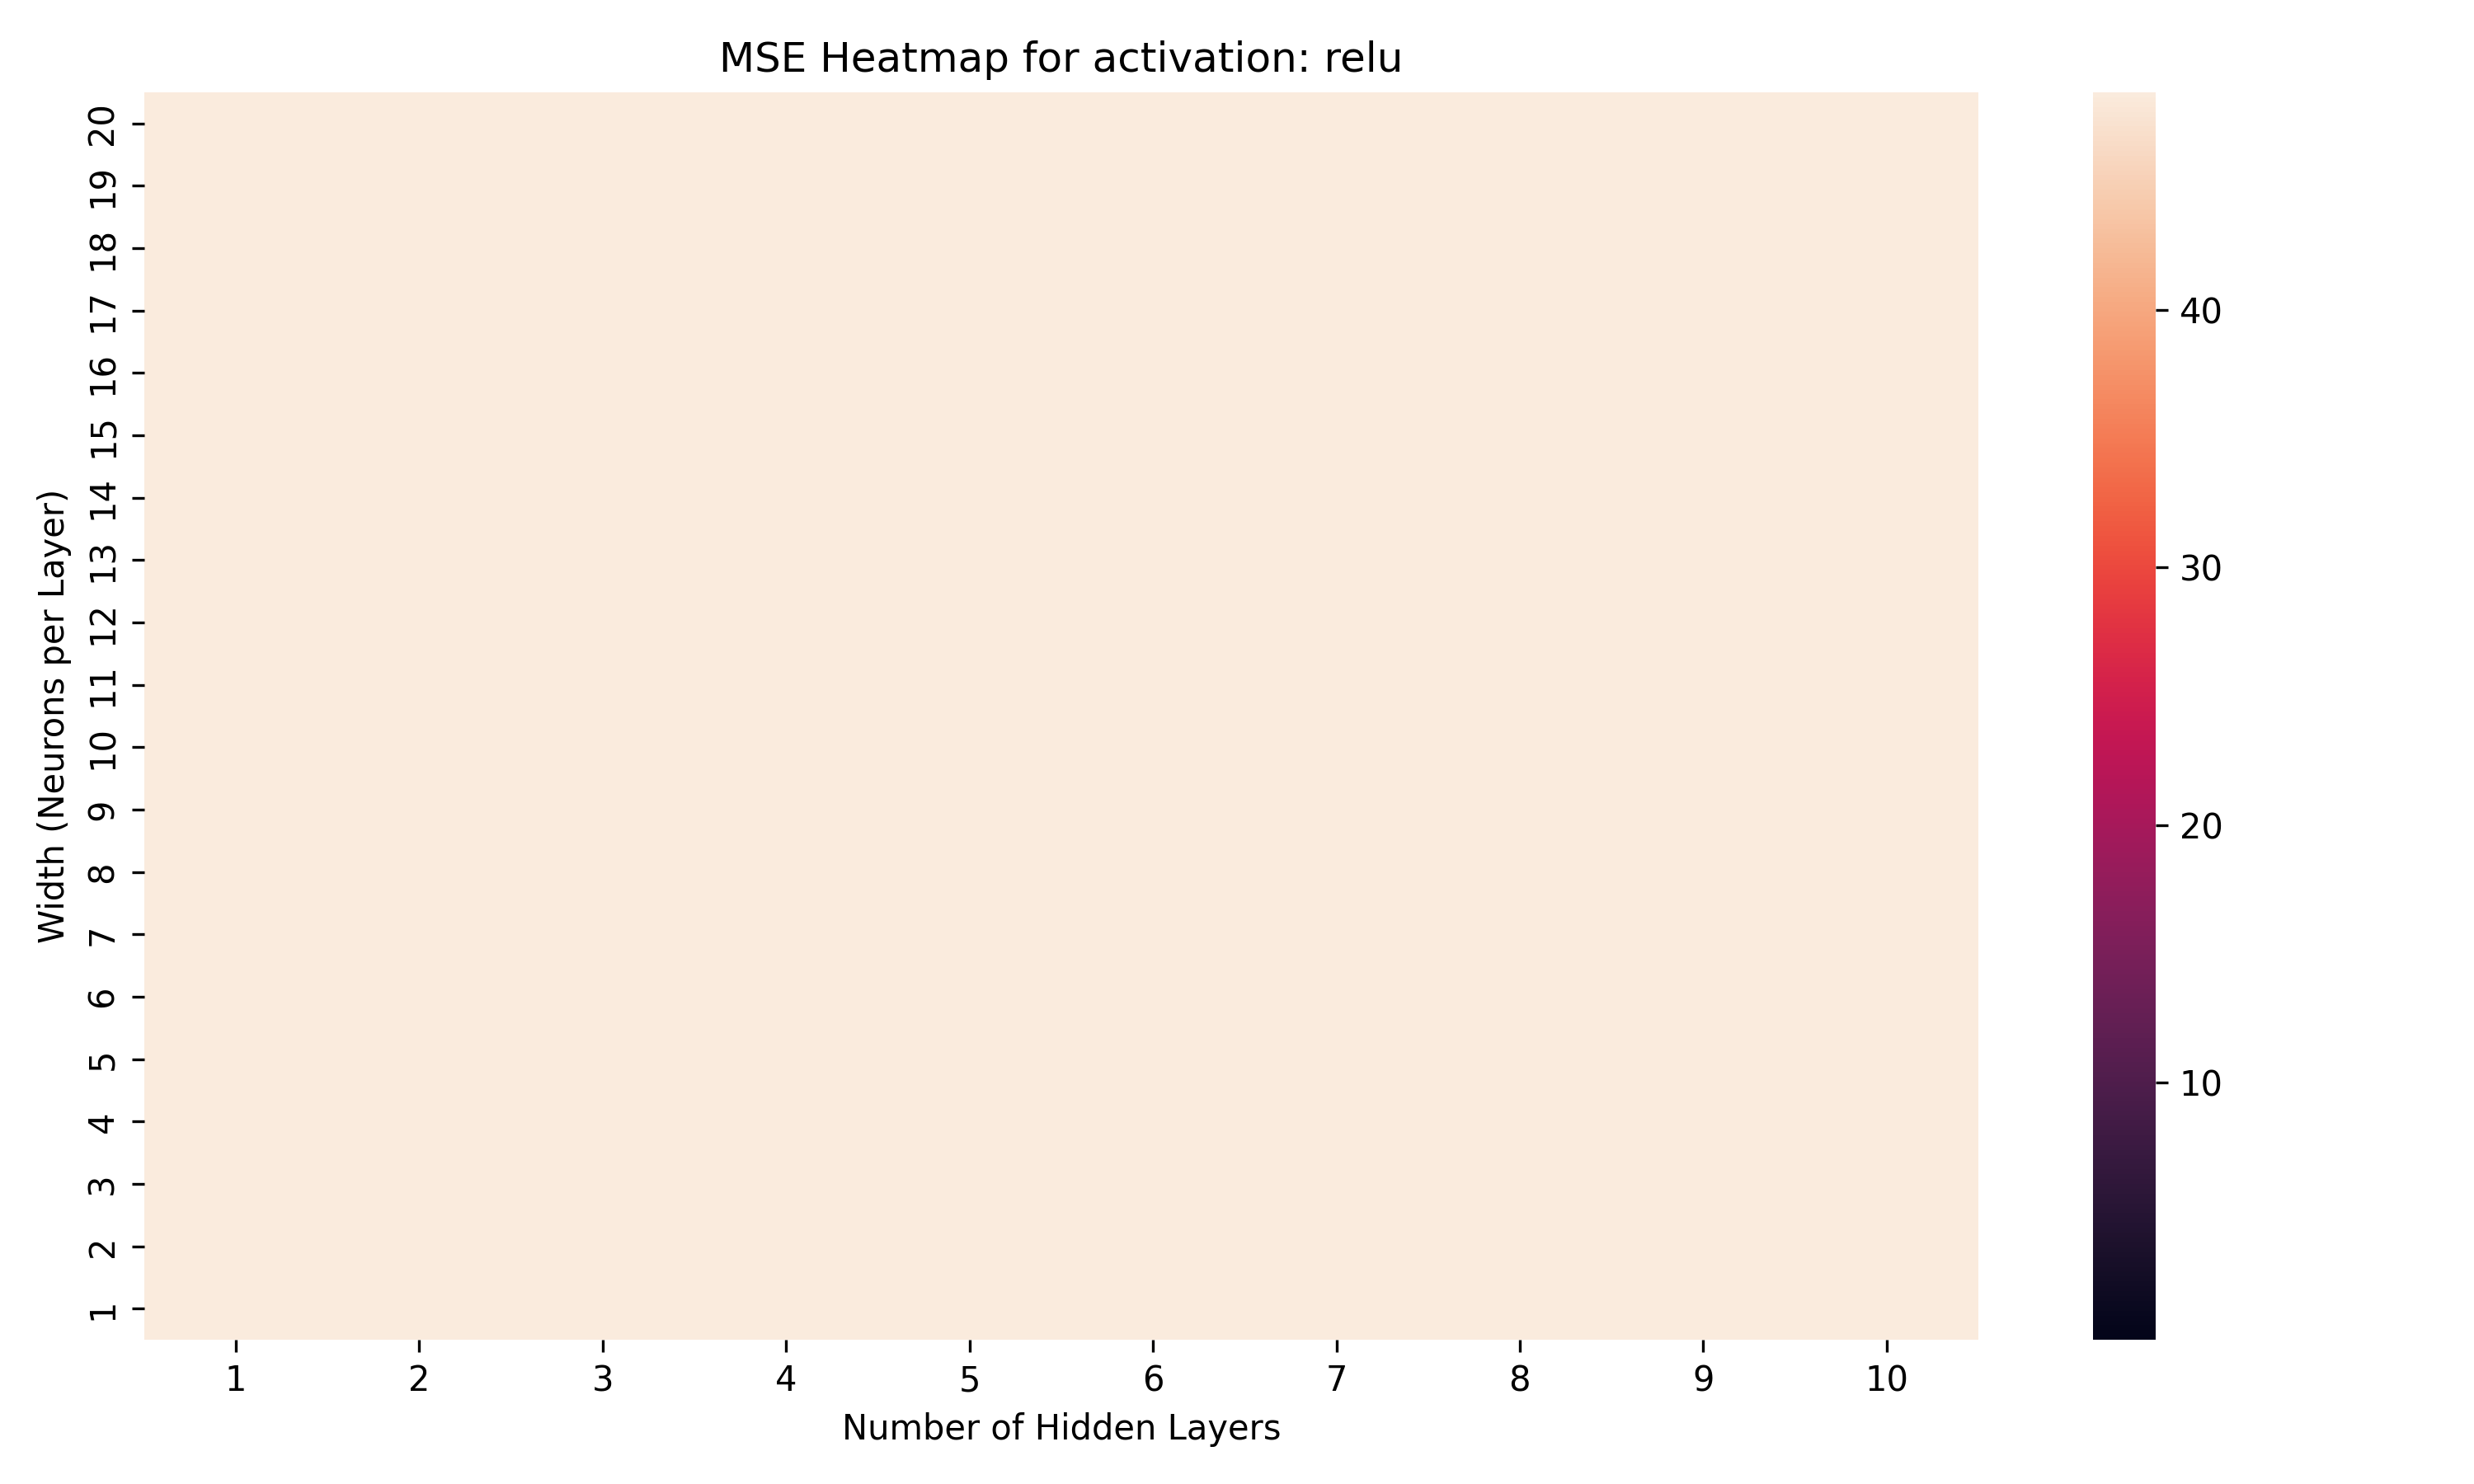
\includegraphics[width=\textwidth]{graphics/mse_heatmap_bvp_poisson_relu.png}
        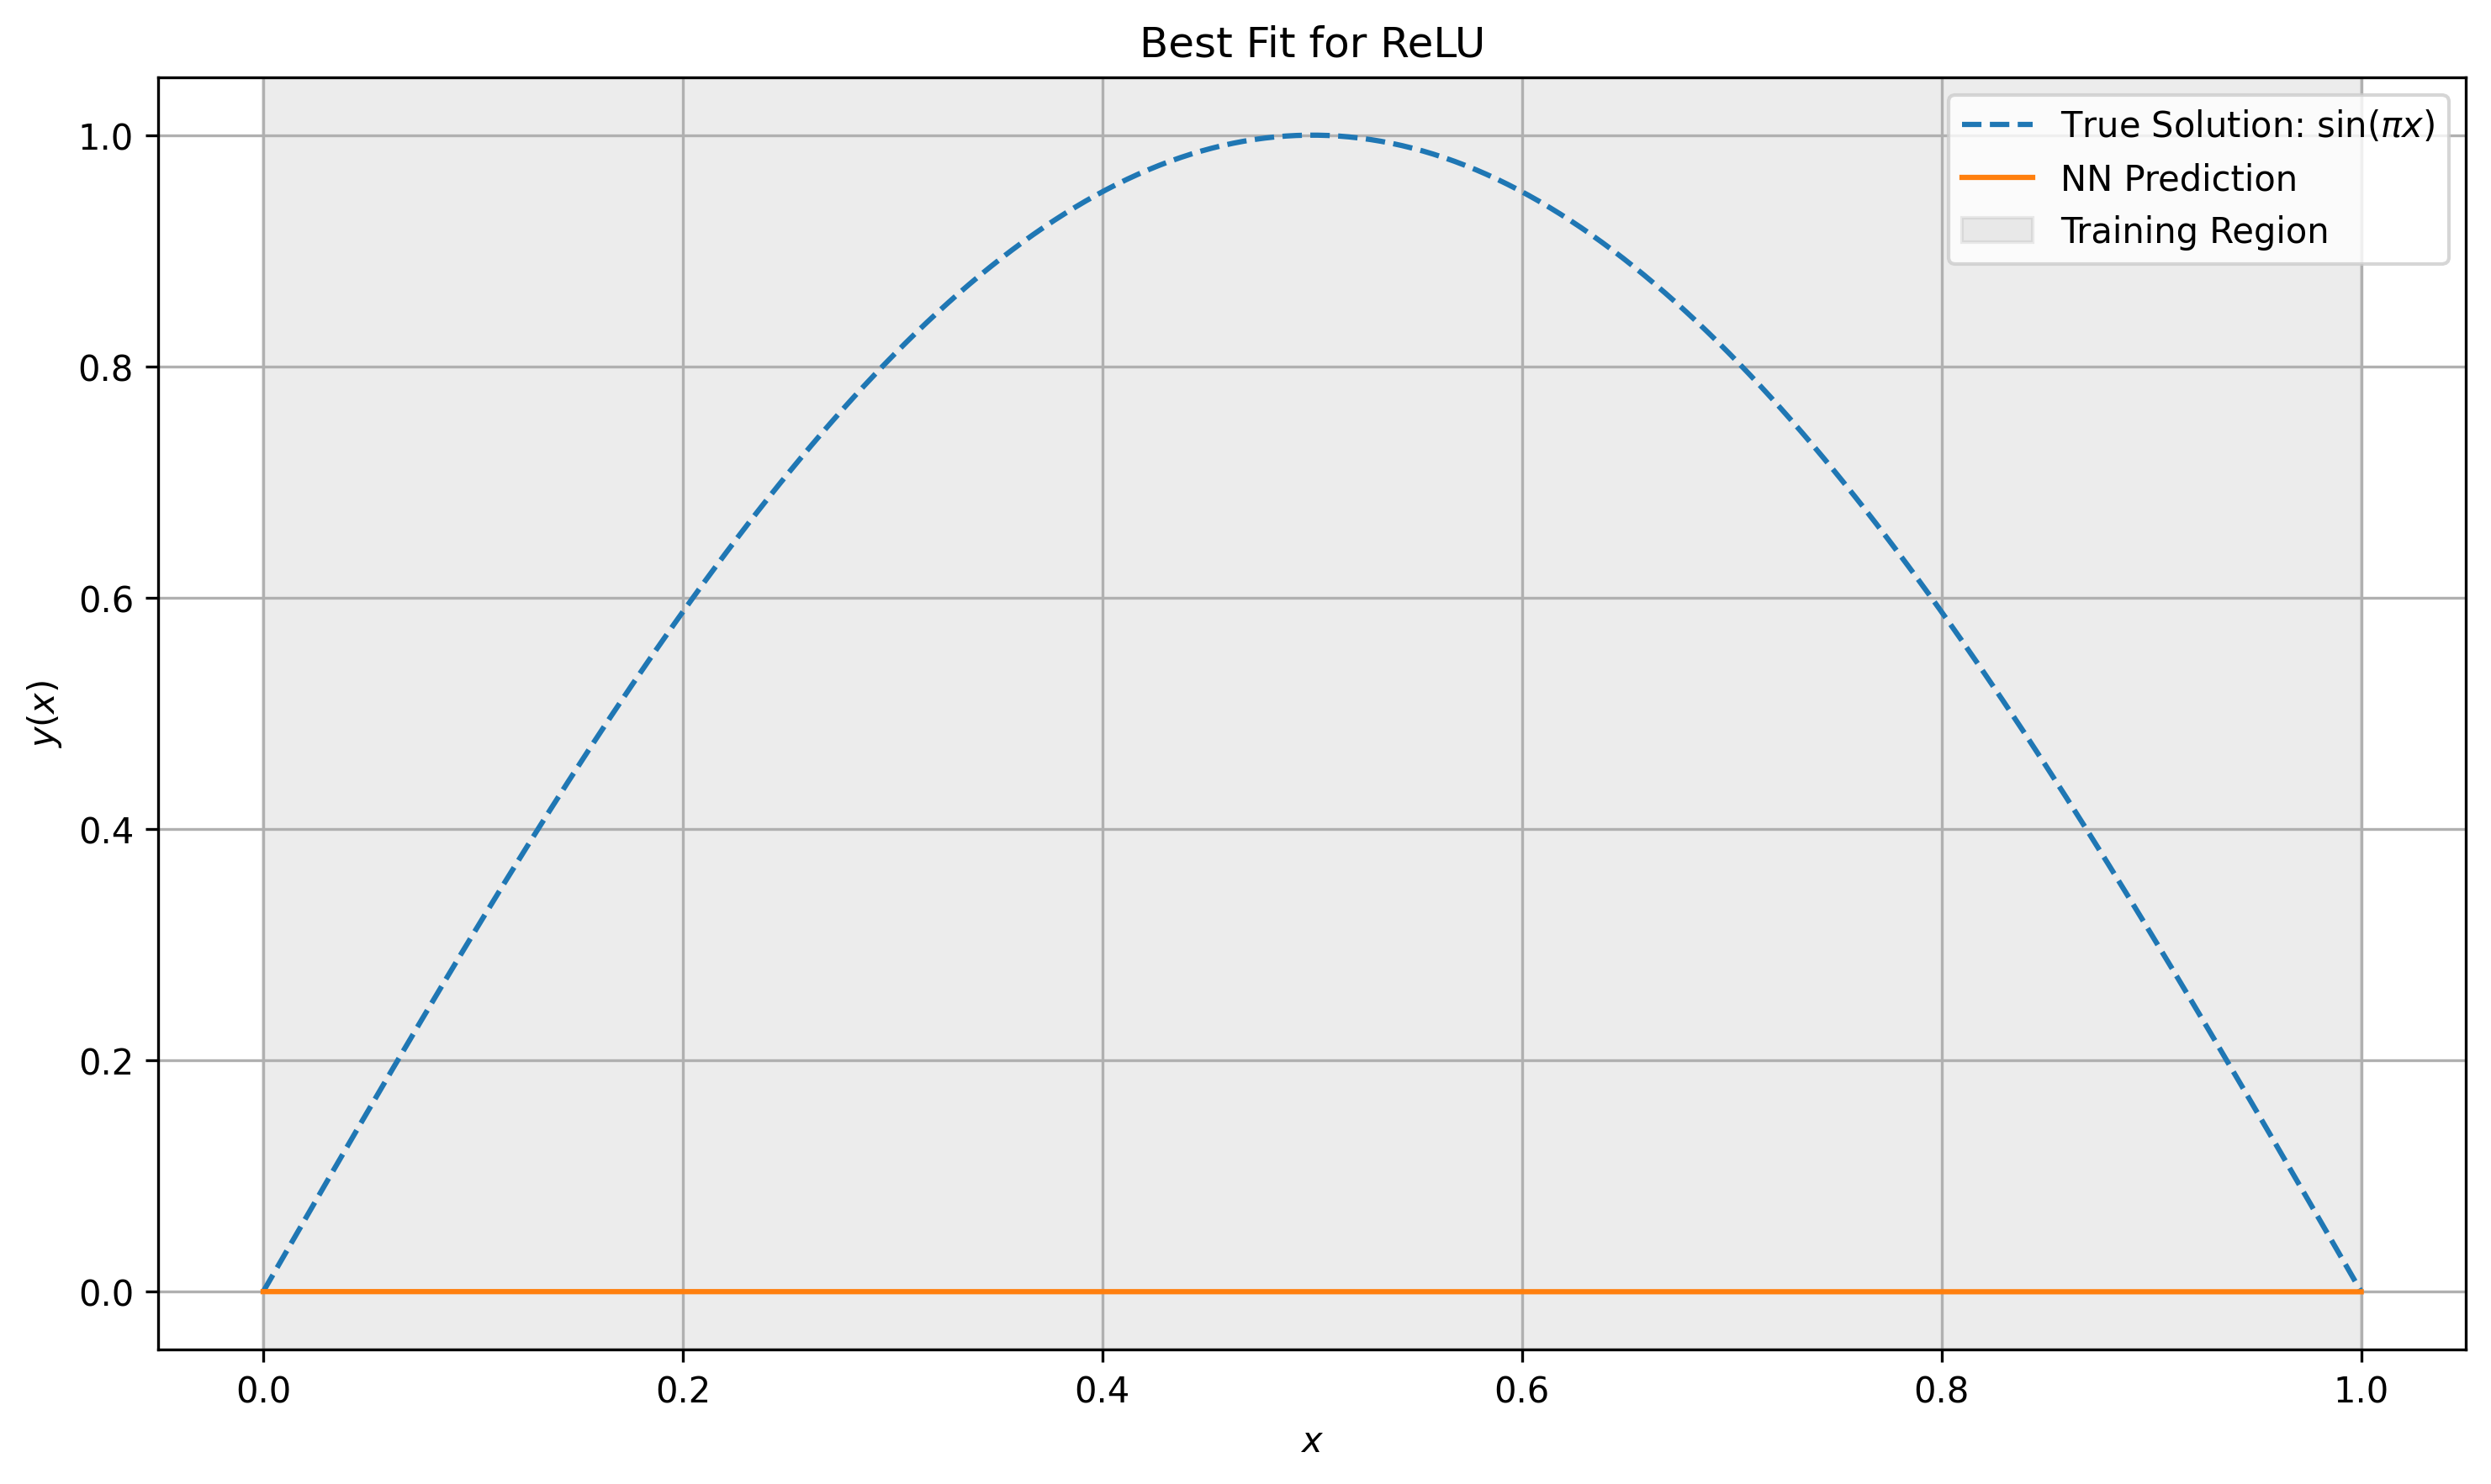
\includegraphics[width=\textwidth]{graphics/bvp_poisson_best_fit_relu_1layers_1width.png}
        \caption{\textbf{ReLU activation.} Heatmap (top), best fit (middle), and worst fit (bottom).}
        \label{fig:ivp_periodic_relu}
    \end{subfigure}
    \hspace*{\fill}
    \caption{Comparison of architectural performance for the exponential decay problem using two 
    activation functions. Each column shows the MSE heatmap with a log error scale,
    the best network fit, and the worst network fit.}
    \label{fig:bvp_poisson_sidebyside}
\end{figure}



\paragraph{Piecewise Forcing}

We now consider a boundary value problem with a discontinuous right-hand side:
\[
\begin{aligned}
    y''(x) &= 
    \begin{cases}
        -1, & 0 \leq x < 0.5, \\
        +1, & 0.5 \leq x \leq 1,
    \end{cases} \\
    y(0) &= 0, \\
    y(1) &= 0.
\end{aligned}
\]
This problem admits a piecewise quadratic solution that is continuous and satisfies the boundary 
conditions. However, the discontinuity in the forcing term results in a derivative jump at 
\( x = 0.5 \), which poses a challenge for smooth neural network approximators.

This example allows us to assess how well neural networks can resolve low-regularity features in 
the solution and adapt to discontinuous dynamics in the governing equation. As before, we 
systematically vary network architecture and activation function, compute the corresponding 
approximation error, and visualise representative results. The best-fitting solutions are 
summarised in Figure~\ref{fig:bvp_piecewise_sidebyside}.

\begin{figure}[h]
    \centering
    \hspace*{\fill}
    \begin{subfigure}[t]{0.48\textwidth}
        \centering
        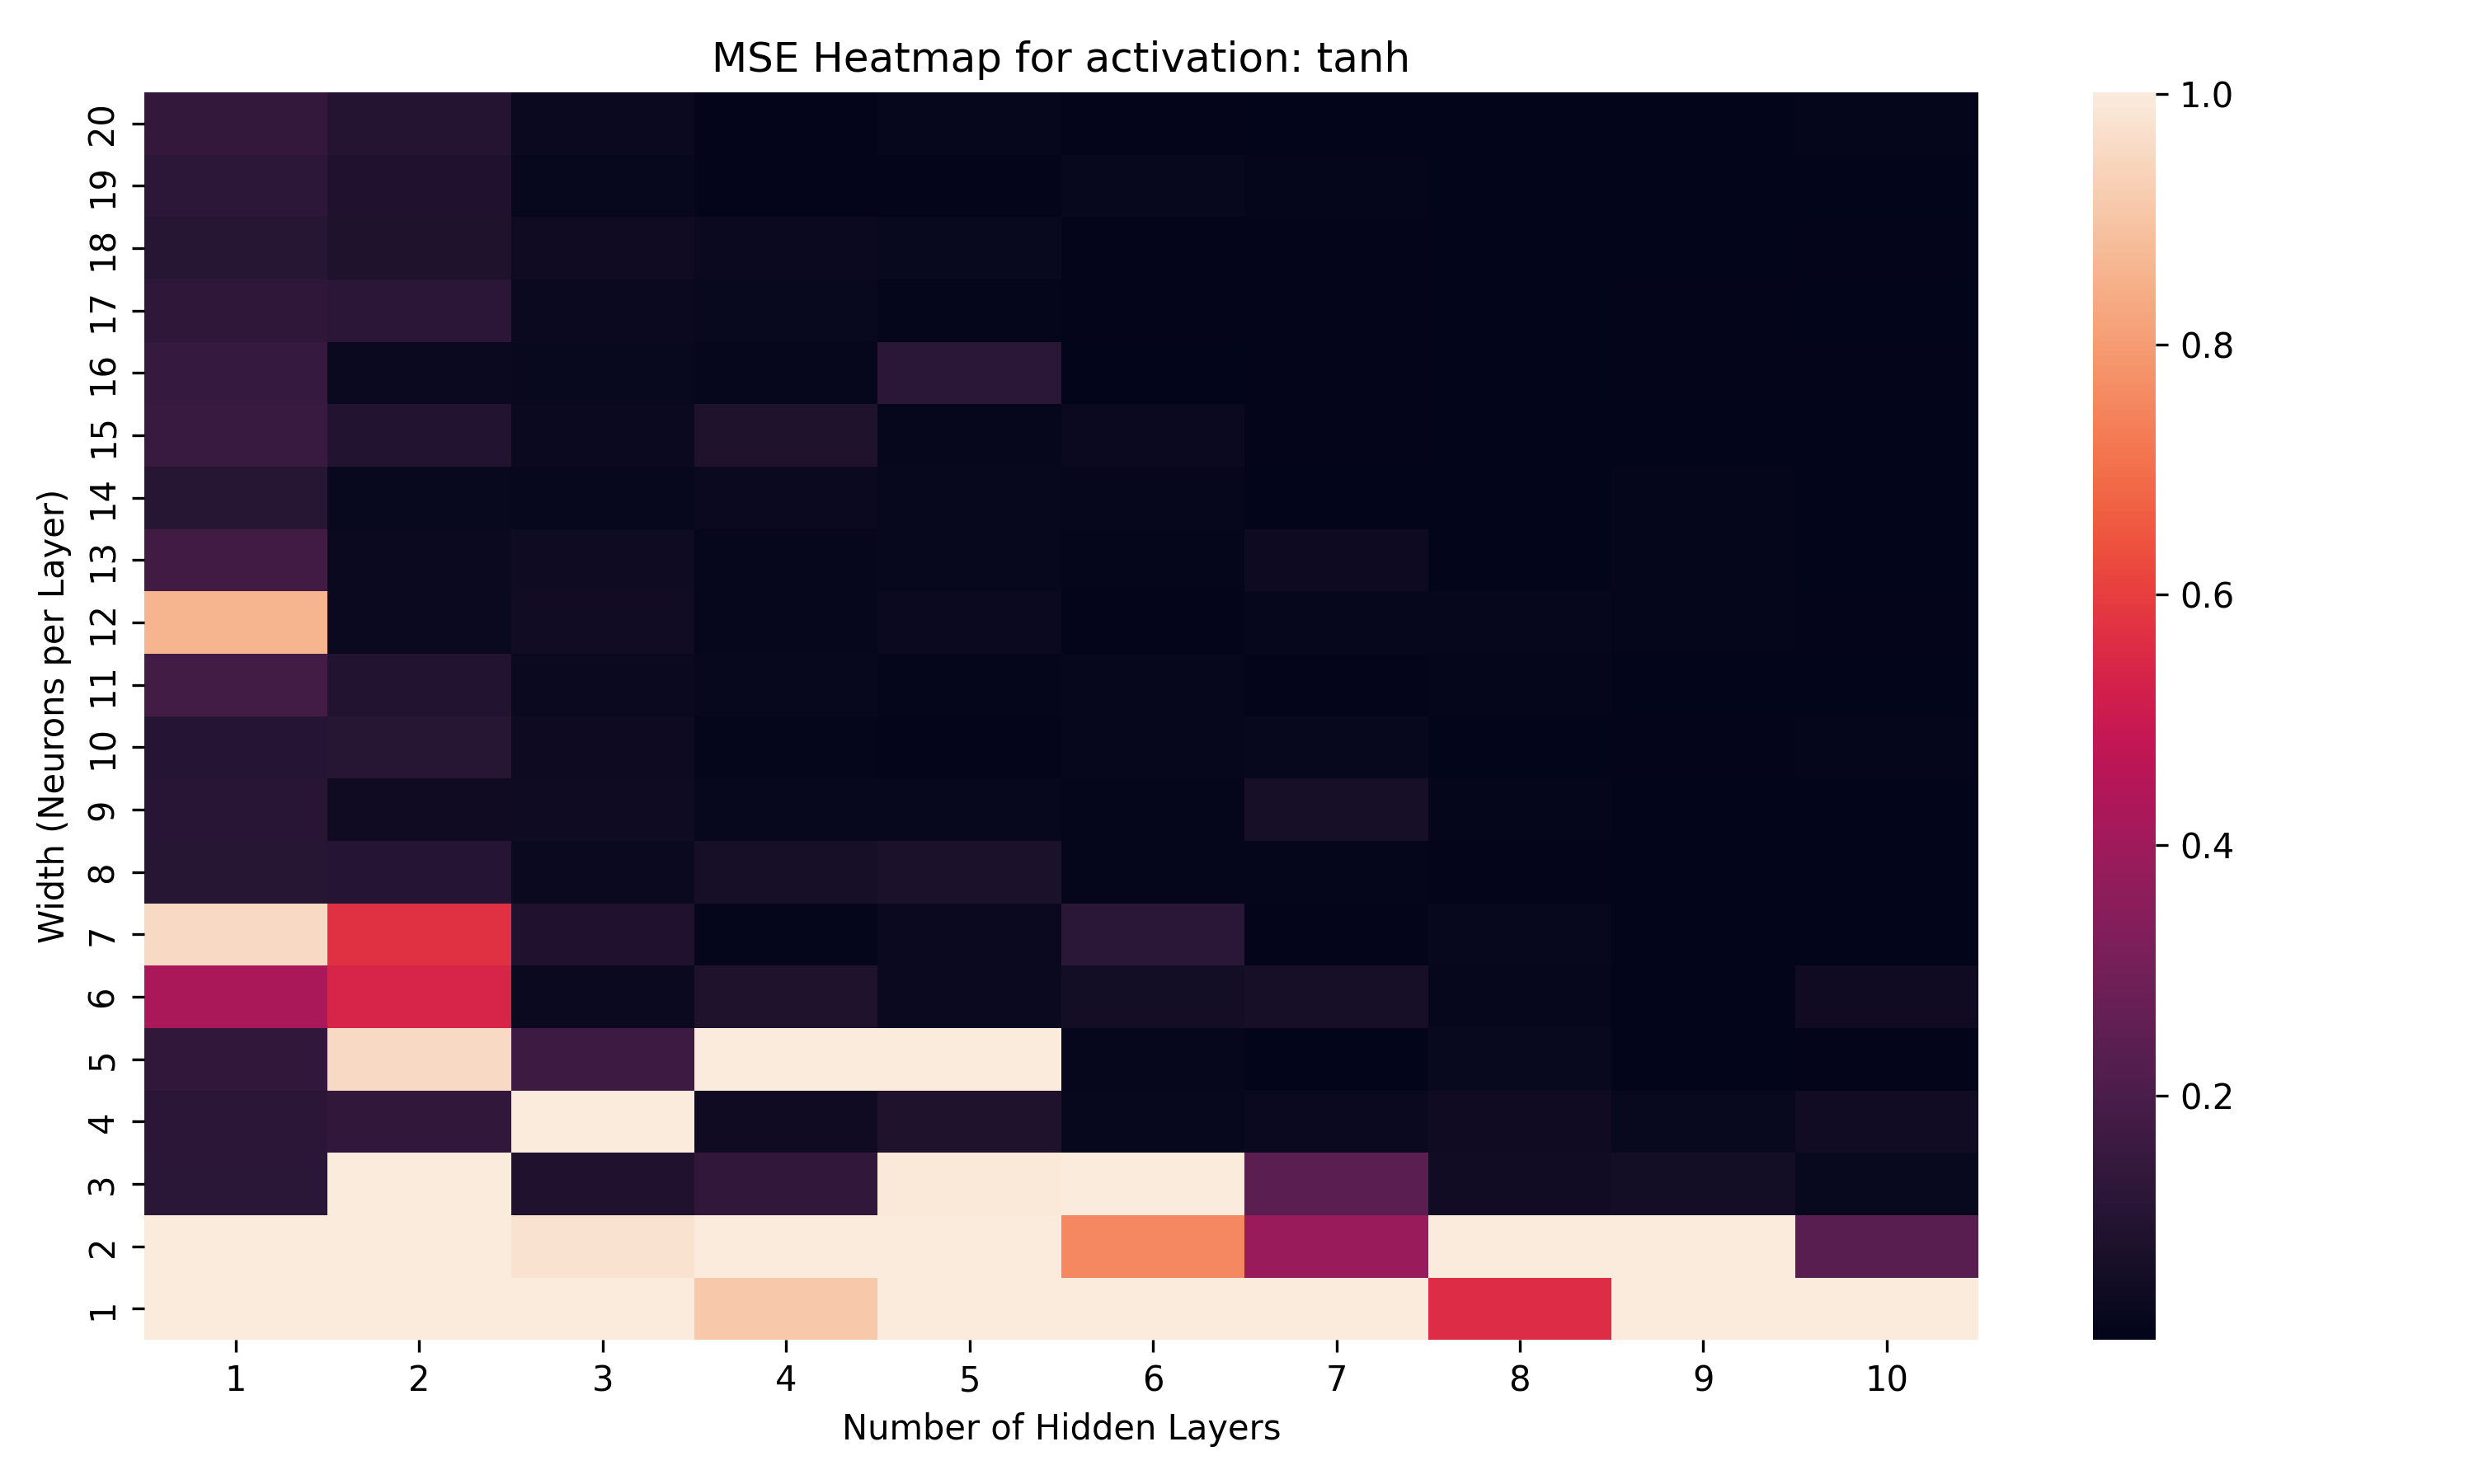
\includegraphics[width=\textwidth]{graphics/mse_heatmap_bvp_piecewise_tanh.png}
        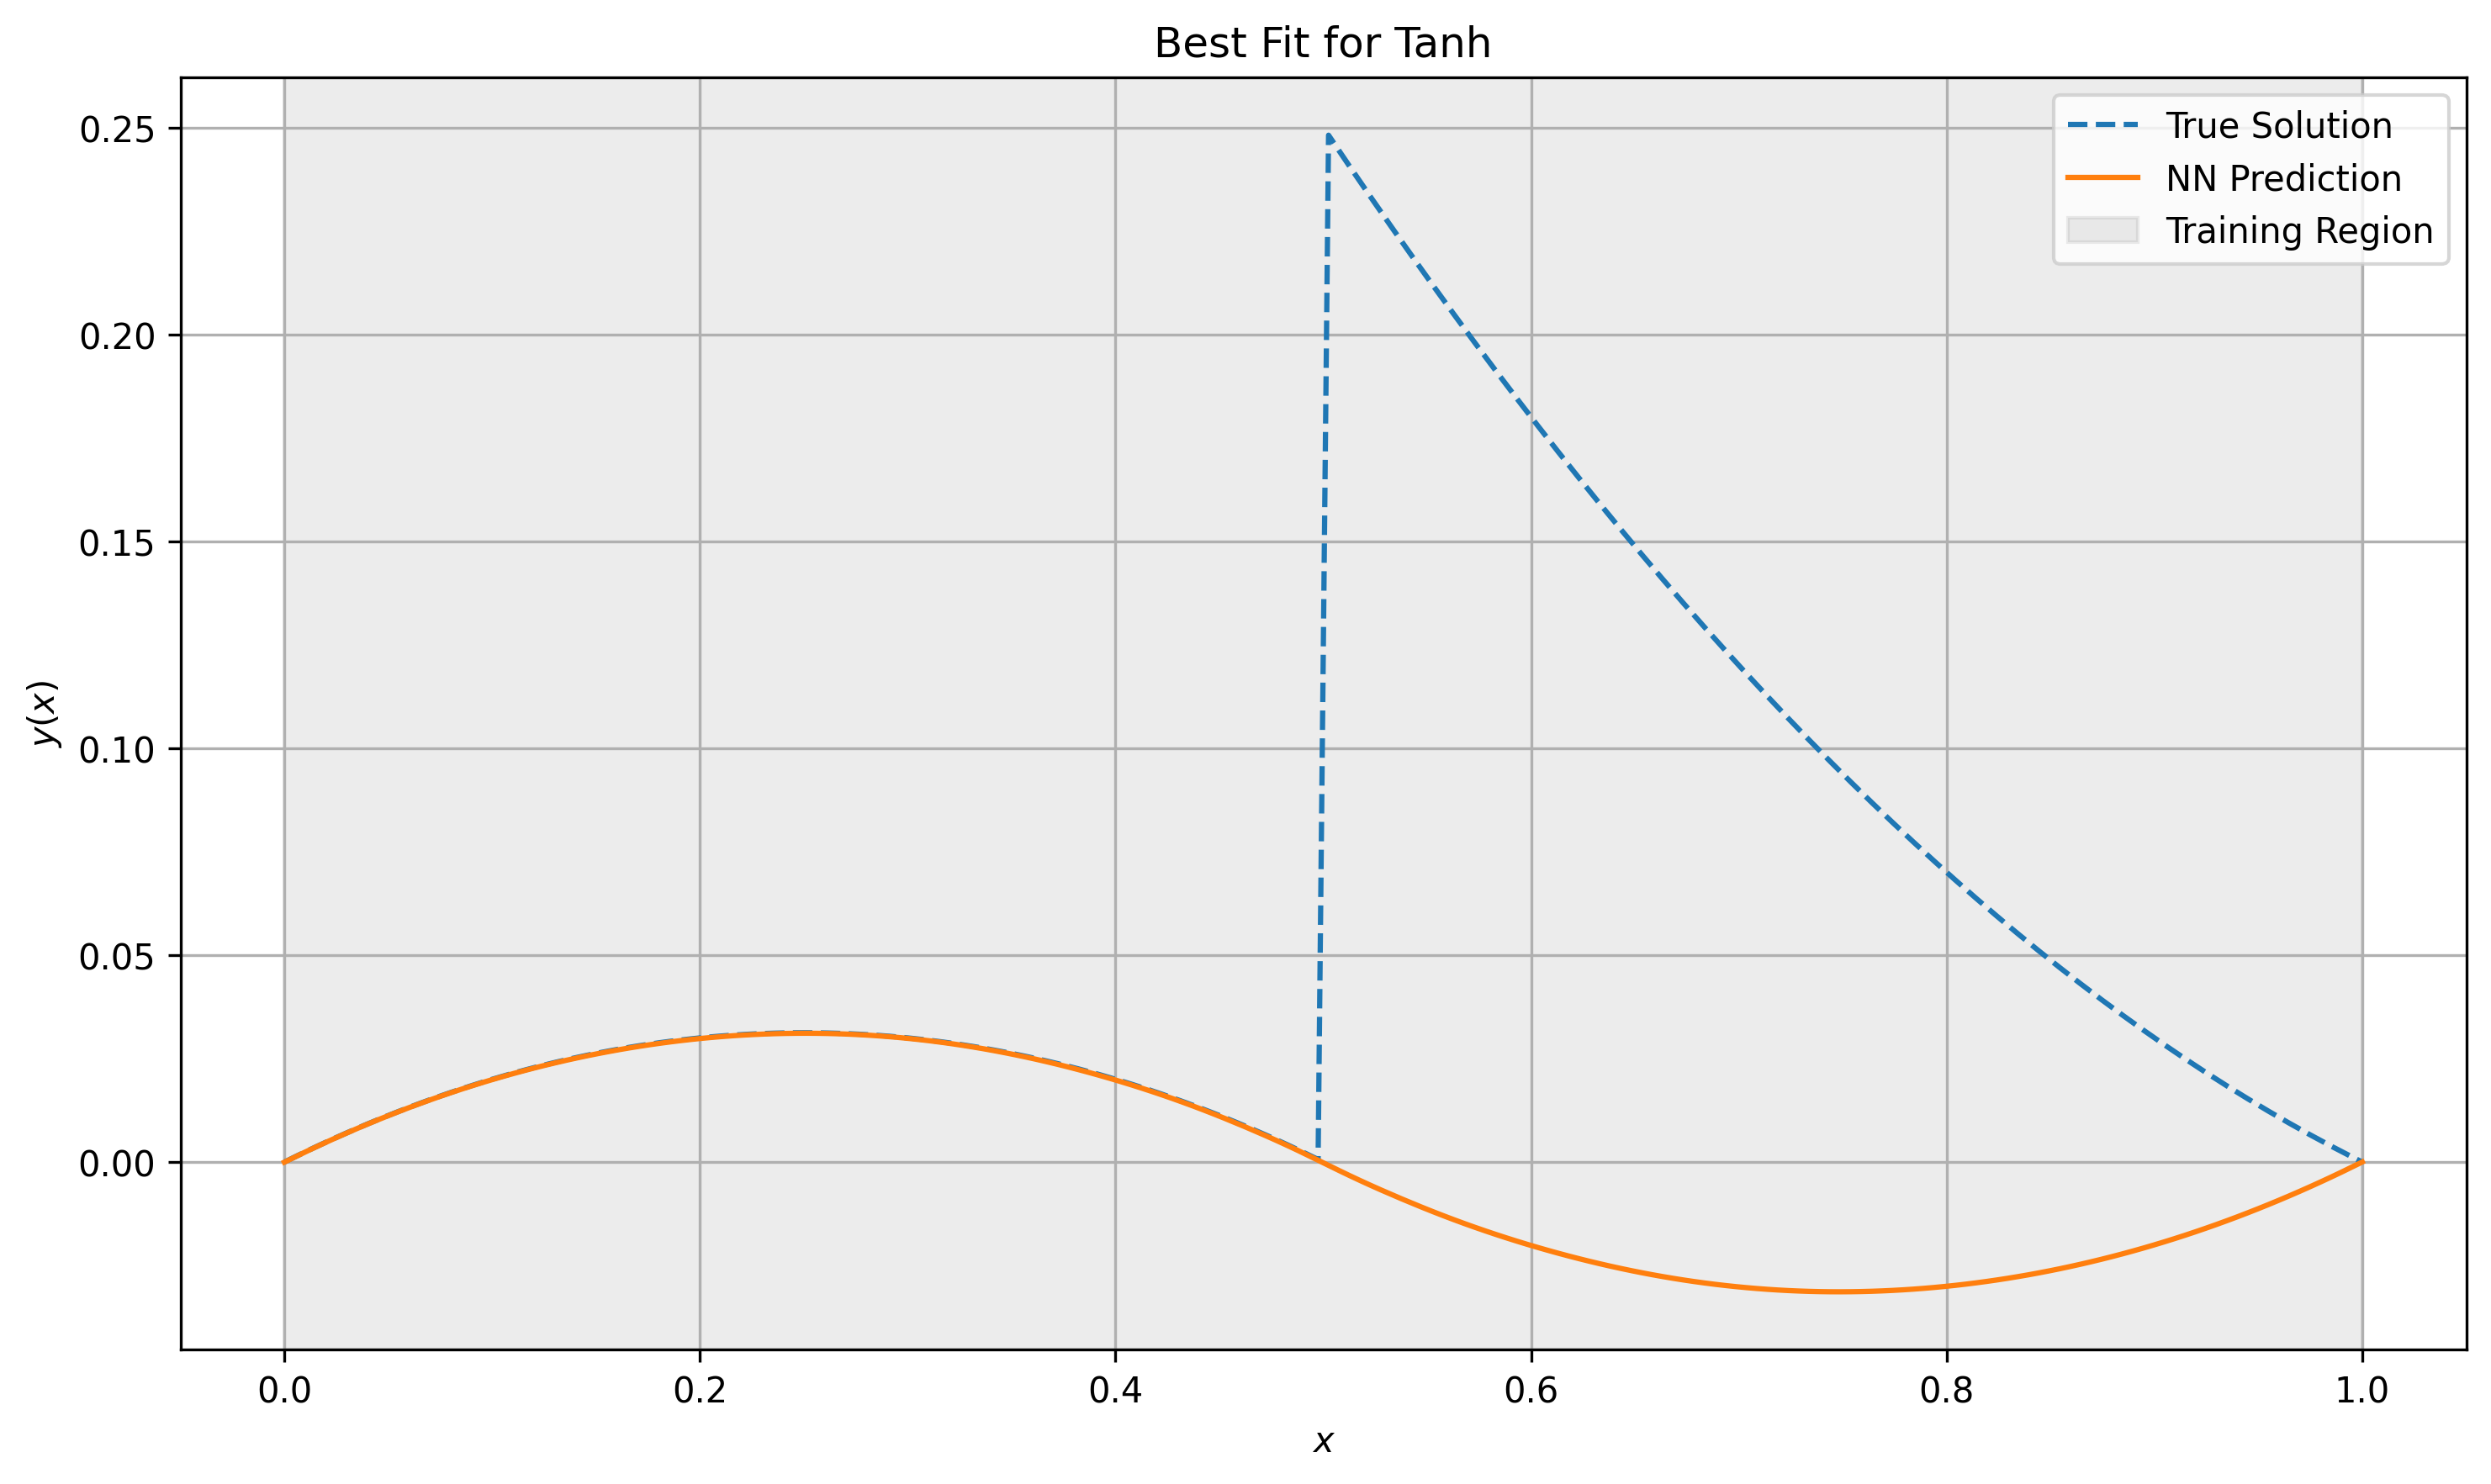
\includegraphics[width=\textwidth]{graphics/bvp_piecewise_best_fit_tanh_10layers_13width.png}
        \caption{\textbf{Tanh activation.} Heatmap (top), best fit (middle), and worst fit (bottom).}
        \label{fig:ivp_periodic_tanh}
    \end{subfigure}
    \hspace*{\fill}
    \begin{subfigure}[t]{0.48\textwidth}
        \centering
        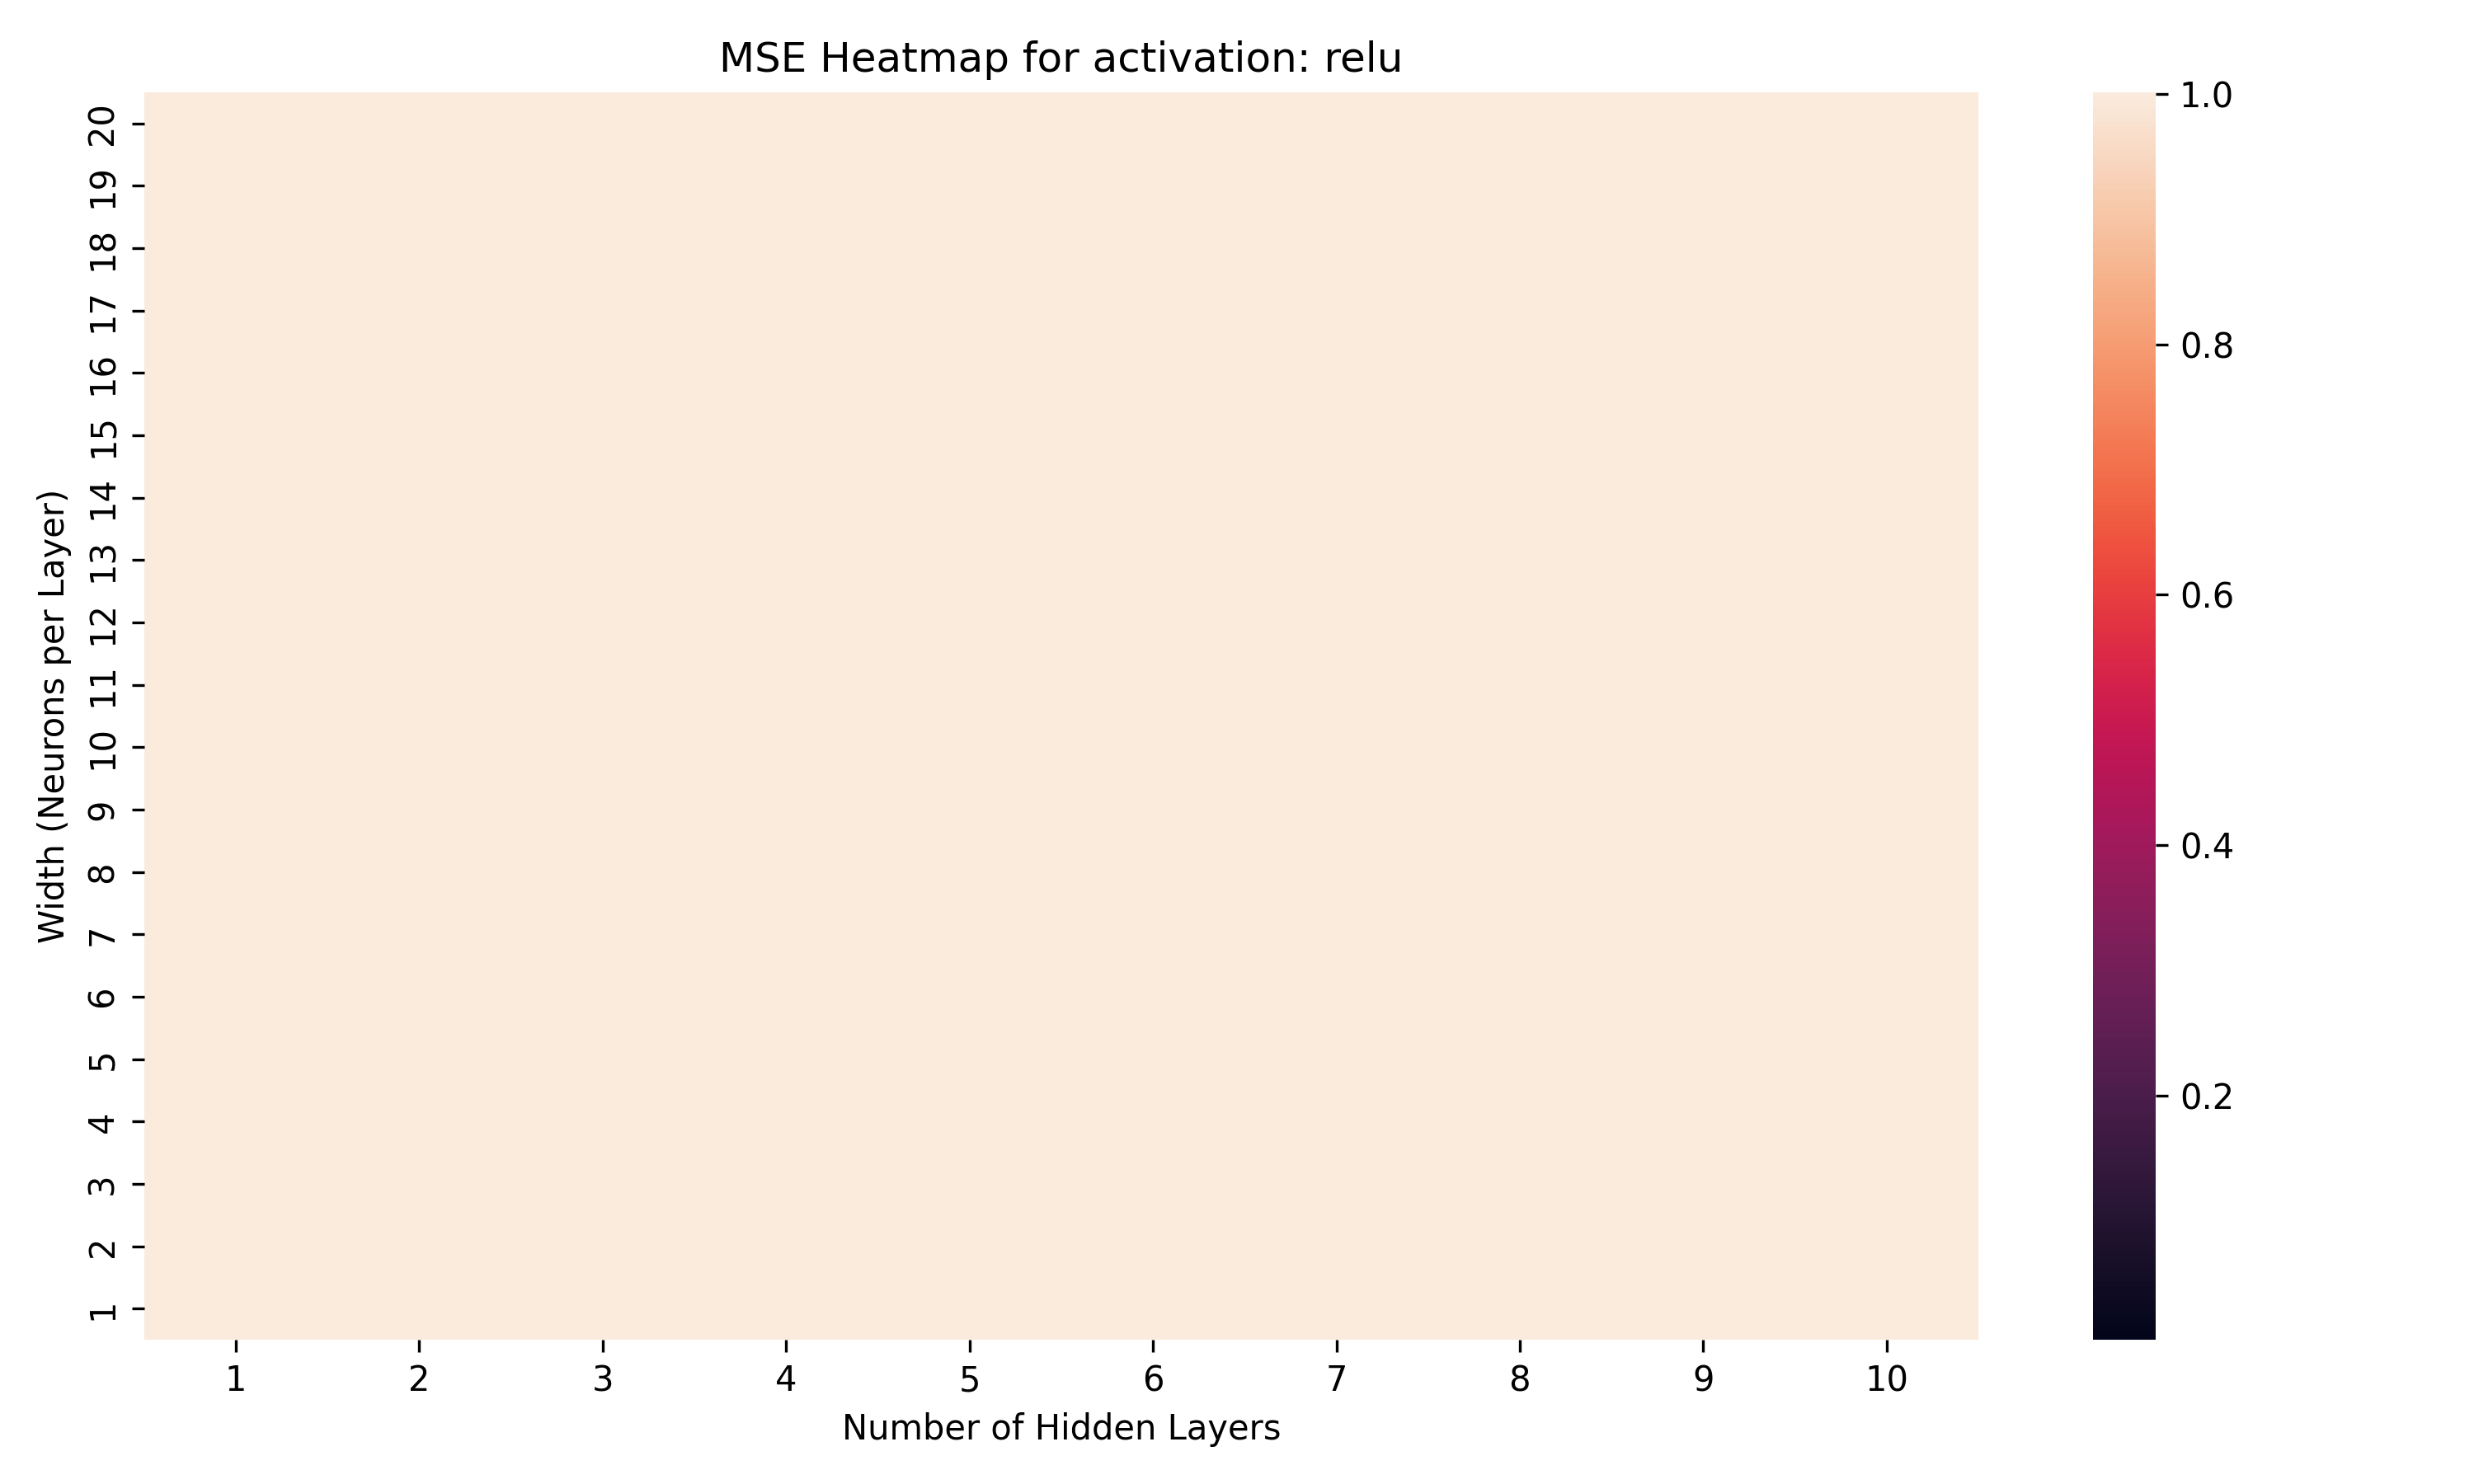
\includegraphics[width=\textwidth]{graphics/mse_heatmap_bvp_piecewise_relu.png}
        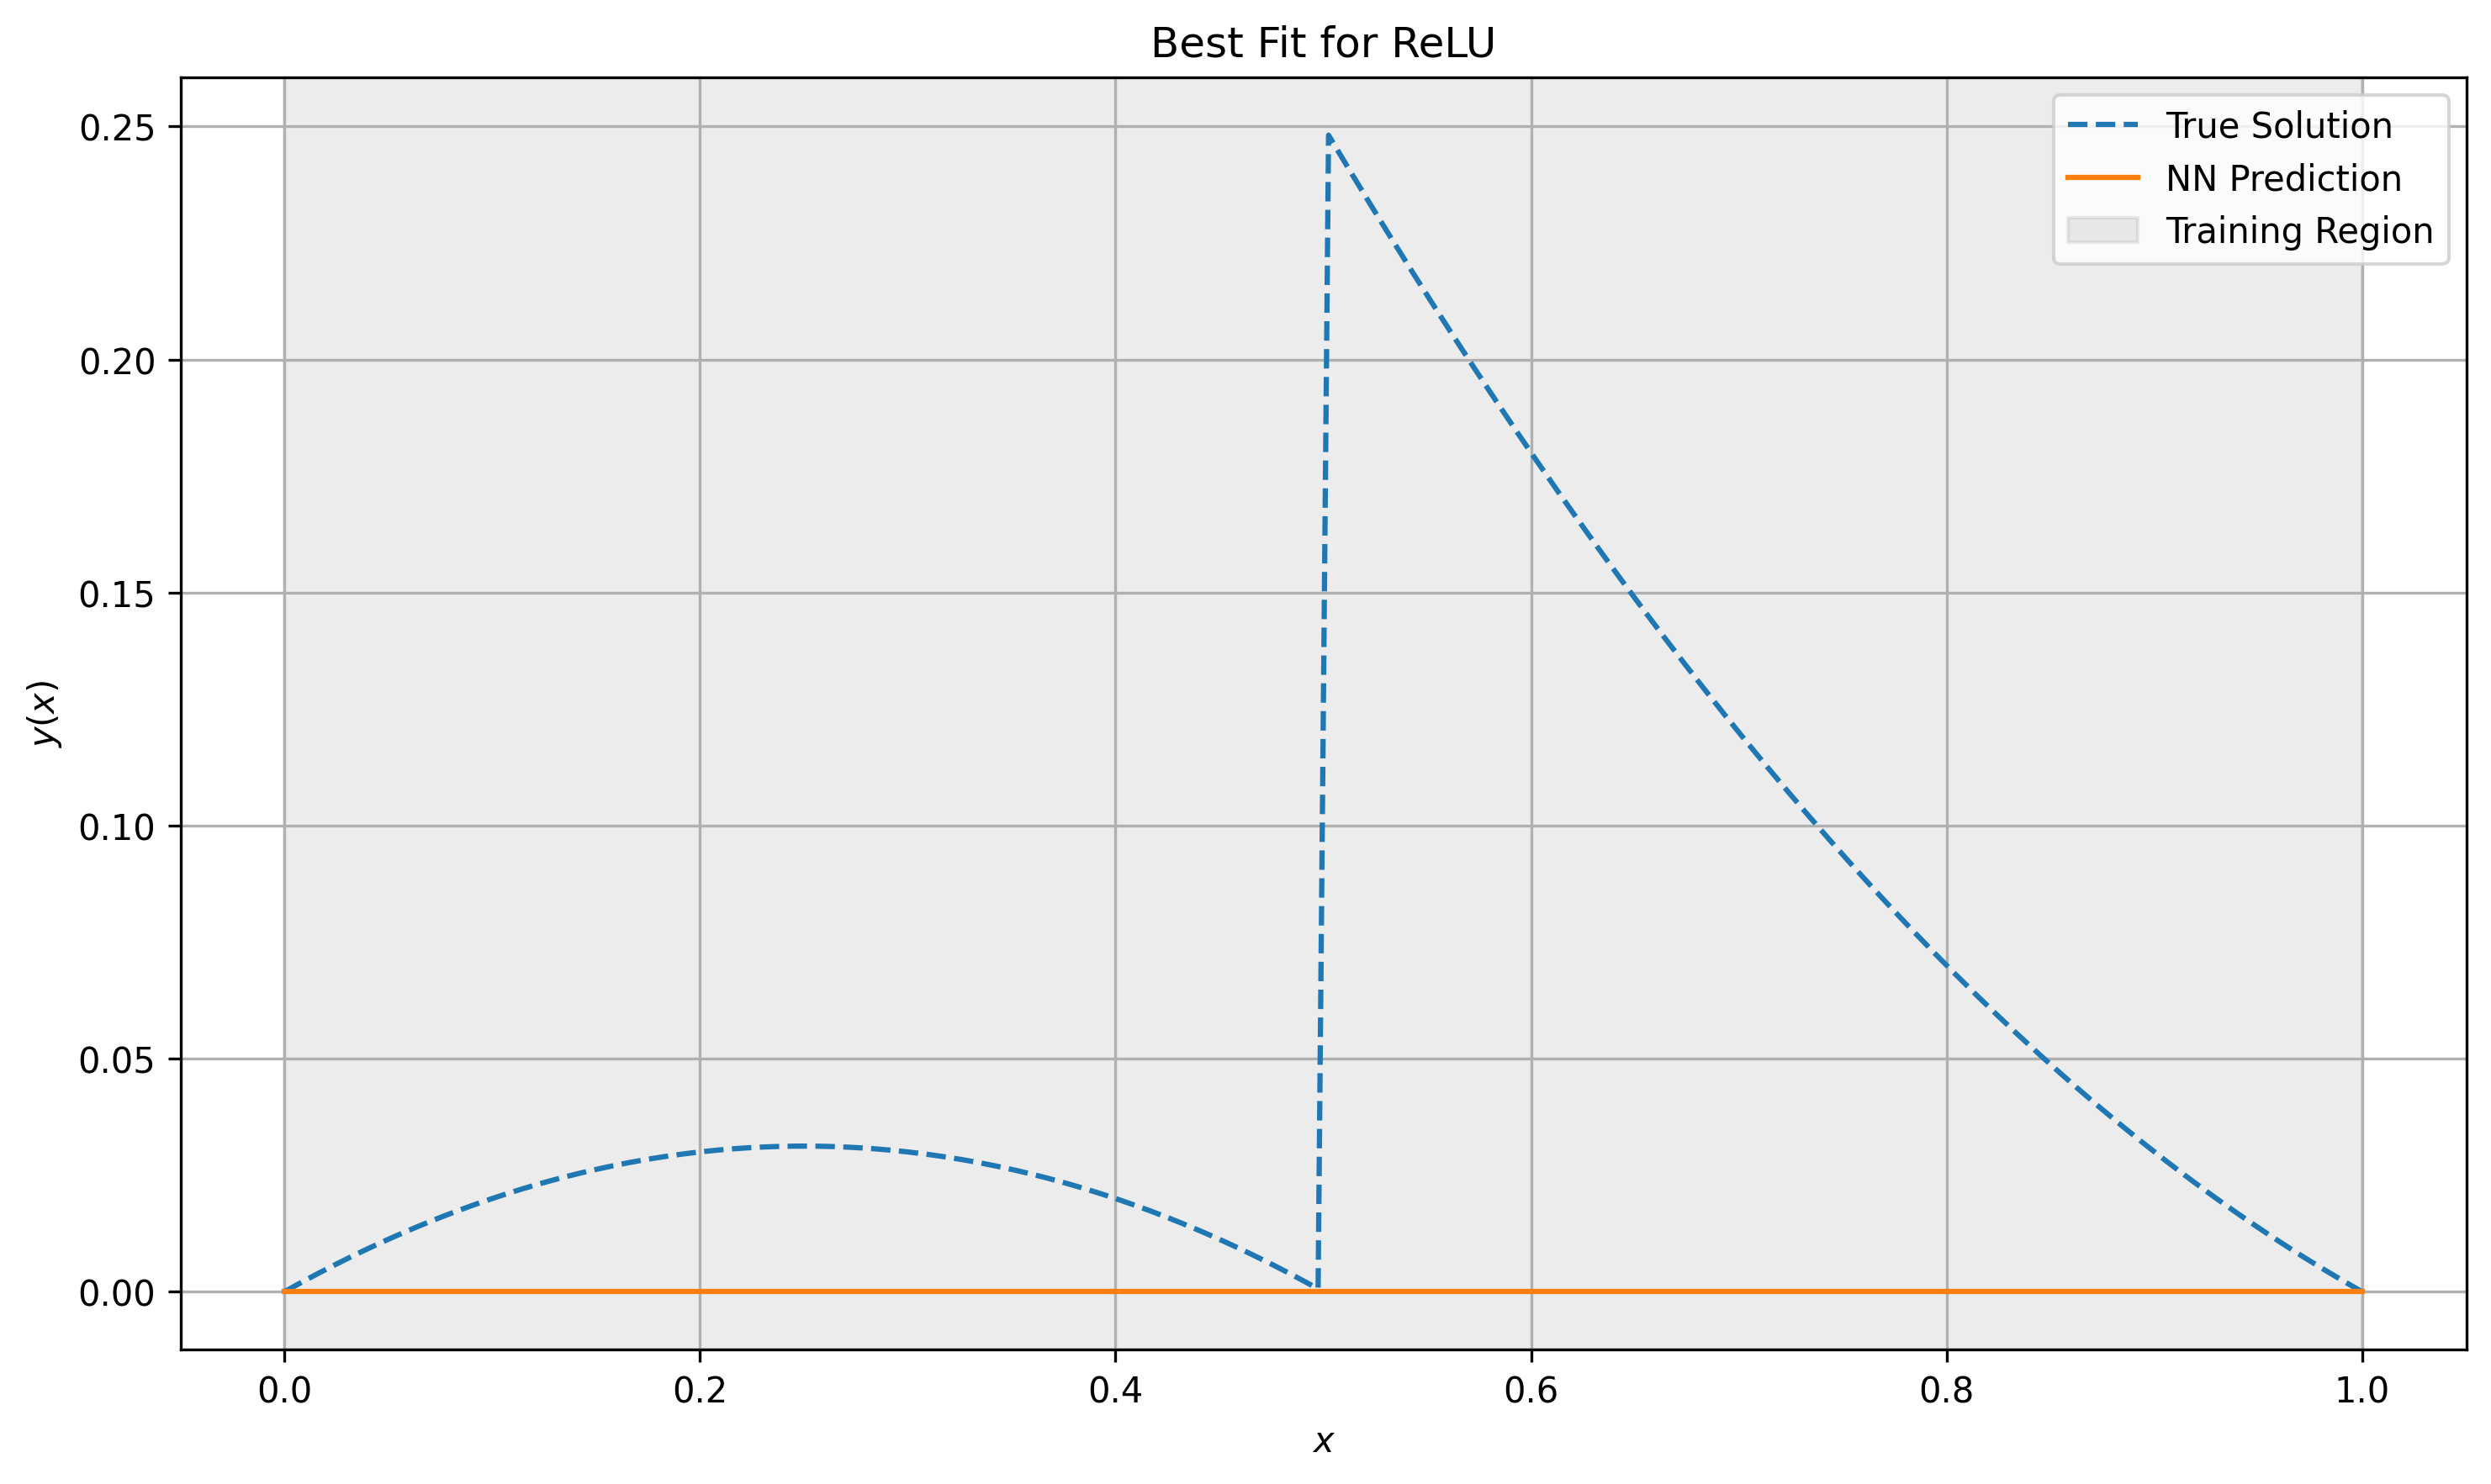
\includegraphics[width=\textwidth]{graphics/bvp_piecewise_best_fit_relu_1layers_1width.png}
        \caption{\textbf{ReLU activation.} Heatmap (top), best fit (middle), and worst fit (bottom).}
        \label{fig:ivp_periodic_relu}
    \end{subfigure}
    \hspace*{\fill}
    \caption{Comparison of architectural performance for the exponential decay problem using two 
    activation functions. Each column shows the MSE heatmap with a log error scale,
    the best network fit, and the worst network fit.}
    \label{fig:bvp_piecewise_sidebyside}
\end{figure}
